%---------------------Settings---------------------------%
\documentclass[10pt,a4paper,twocolumn,twoside,UTF8]{article}
\usepackage{geometry}
	\geometry{left=1.8cm,right=1.8cm,top=2.5cm,bottom=2cm}
% \usepackage{xeCJK}
\usepackage{amsmath,paralist,enumitem,booktabs,multirow,graphicx,subfig,setspace,listings,multicol,lettrine}
	\setlength{\parindent}{2em}
	\lstset{language=Python}
\usepackage{fancyhdr}
\usepackage{layout}
\setlength\columnsep{0.8cm}

%%begin----------Set header and footer----------------%%
\usepackage{ifthen}
\newboolean{first}
\setboolean{first}{true}
\pagestyle{fancy}
	\fancypagestyle{maincontent}{
		\fancyhf{}  
		\fancyhead[EL, OR]{\thepage}
		\fancyhead[EC]{C9 Unravel the general characteristics of chaotic systems by exploring chaotic circuits}
		\fancyhead[OC]{GENERAL PHYSICS LABORATORY}
		\renewcommand\headrulewidth{0pt}
	}
	
	\usepackage{datetime}
	\fancypagestyle{firstpage}{
		\setboolean{first}{false}
		\fancyhf{}  
		\fancyhead[L]{Sun Yat-sen University}
		\fancyhead[R]{\shortmonthname[\the\month], \the\year}
		\fancyhead[C]{
		          \large{GENERAL PHYSICS LABORATORY}
		          }
	}
	
	\newcommand{\makefirstpageheadrule}{
	\makebox[0pt][s]{\rule[0.6\baselineskip]{\headwidth}{0.3pt}}
	\makebox[0pt][s]{\protect\hspace{-0.34em}\rule[0.75\baselineskip]{\headwidth}{0.3pt}}
	\protect\vspace{-20pt}
	}

	\newcommand{\makeheadrule}{
	\makebox[0pt][l]{\rule[1\baselineskip]{\headwidth}{0.3pt}}
	\protect\vspace{-20pt}
	}

	\renewcommand{\headrule}{
	\ifthenelse{\boolean{first}}{\makeheadrule}
	{\makefirstpageheadrule}
	}
%%end--------------Set header and footer-----------%%

%%begin-----------------Reference-----------------------%%
\usepackage[colorlinks,linkcolor=blue,urlcolor=blue,citecolor=blue]{hyperref}
\usepackage[hyperref=true,backend=biber,bibstyle=science,citestyle=numeric-comp,sorting=none,backref=true]{biblatex}
\addbibresource{REF.bib}
%%end-------------------Reference-----------------------%%

%end---------------------Settings---------------------------%




%%%%%%%%%%%%%%%%%%%%%%%%%%%%%%%%%%%%%%%%%%%%%%%%%%%%%%%%%%
%%%%%%%%%%%%%%%%%%%%%%%%%Document%%%%%%%%%%%%%%%%%%%%%%%%%
%%%%%%%%%%%%%%%%%%%%%%%%%%%%%%%%%%%%%%%%%%%%%%%%%%%%%%%%%%

%%begin-------------------Abstract-----------------------%%
\begin{document}
\title{\LARGE\textbf{Unravel the general characteristics of chaotic systems by exploring chaotic circuits} \footnotemark[1]}
\author{\large\textit{Zweig, Wong}$^{1}$\footnotemark[2]
\\ \normalsize{1 Zhongshan School of Medicine, Sun Yat-sen University, Guangzhou  { \rm 510275}, China}}
\date{}

\twocolumn[
	\begin{@twocolumnfalse}
	\maketitle  
	\renewcommand{\abstractname} {} 
	\begin{abstract}
	\vspace{-3em}
	{\bf Abstract: }
	{\small 
    Chaos theory is a branch of non-linear mechanics that focuses on underlying patterns and deterministic laws of non-linear dynamical systems which generally have complex and unpredictable oscillation patterns. 
	It is important to unravel the principles and general characteristics of these chaotic systems, and chaotic circuits are ideal models for demonstrating and exploring chaotic phenomena. 
	In this research, we delved into two chaotic circuits, the Chua's chaotic circuit and Lorentz's chaotic circuit, 
	by doing numerical calculations, developing simulation circuit models, and conducting real-world circuit experiments. 
	We found that both circuits have very complex chaotic patterns. 
	For instance, in Chua's circuit experiment we found oscillation patterns including straight line, limiting ring, double-attractor, and single attractor. 
	These patterns were mutually verified in all three experiments.
	The results proved that the behaviors of chaotic systems are highly sensitive to initial conditions, but they are preciously determined by the physical laws, 
	and, although the exact behaviors are unpredictable, the general pattern seems constant under a certain condition. 
	In conclusion, in this experiment, we investigated the properties of different oscillation patterns of chaotic circuits and deepened our understanding of the general principles of chaotic systems. 
	Our work might pave the way for further research of chaotic systems.
	}
	\par
	\textbf{Keywords: Chaos theory, Chua's chaotic circuit, Lorentz's chaotic circuit, Circuit simulation} 
	\vspace{2em}
	\end{abstract}
	\end{@twocolumnfalse}
]

\renewcommand{\thefootnote}{\fnsymbol{footnote}}
\footnotetext[1]{Supported and taught by Luyoutang, School of Physics, Sun Yat-sen University}
\footnotetext[2]{Corresponding author. ID: 20980066 Email: \url{huangzw29@mail2.sysu.edu.cn} }
%%end-------------------Abstract-----------------------%%

\thispagestyle{firstpage} 
\pagestyle{maincontent}

%%begin-------------------Intro-----------------------%%
\section{Introduction}
\lettrine[lines=2]{C}{haos} theory is a branch of non-linear mechanics which focuses on the underlying patterns and deterministic laws of complex non-linear dynamical systems.
It has been widely acknowledged that these systems appear to have states of extreme disorder and irregularities and are usually unpredictable and highly sensitive to initial conditions.
The chaos theory states that although behaviors of these systems are complex and unpredictable, they are not completely random. 
Instead, they are exactly determined by certain physical laws and, within the apparent randomness, 
there are underlying patterns that show interconnectedness, constant feedback loops, repetition, fractals, self-similarity, and self-organization\autocite{sekarChaosMechanicalSystems1995}.

The theory has undergone rapid development in the past century and has recently gained more and more attention in other fields such as 
ecology\autocite{yinConstructingPostClassicalEcosystems2011} and medicine\autocite{oestreicherHistoryChaosTheory2007}.
It has gone further beyond physics and became an interdisciplinary scientific theory nowadays.
Thus, it is important to unravel the principles and general characteristics of the chaotic system.

One of the simplest and easiest-to-construct chaotic system is chaotic electronic circuits. 
They are circuits containing nonlinear electronic components and thus demonstrate various chaotic oscillation patterns that respond to different parameters and show all important aspects of the chaotic theory,
which makes them ideal and effective models for studying the chaotic phenomena.
In fact, when investigating other much more complex chaotic systems, it is a pretty effective way to create and operate on an electronic "analog" instead of directly working with the actual system, which may be difficult or impossible to control, e.g. the human body.

In this study, we will focus on two classical chaotic circuits, Chua's chaotic circuit and Lorentz's chaotic circuit,
and investigate the properties of different oscillation patterns by conducting numerical calculations, simulation, and real-world circuit experiments.

%%end-------------------Intro-----------------------%%
% \newpage % Change the column
%%begin-----------------Method-----------------------%%
\section{Experimental principles and method}
	\subsection{Experimental principle}
		\subsubsection{General characteristics of chaotic oscillation in the non-linear dynamics system\autocite{shenGeneralPhysicsLaboratory2015}}
		
		A deterministic dynamical system has three common stable states: equilibrium, periodic oscillation, and quasi-periodic oscillation states.
		
		Chaotic oscillation is an unstable but finite dynamical oscillatory behavior. It generally has the following properties:
		
		\begin{enumerate}[label=\arabic*.]
			\item The state is extremely sensitive to the initial conditions of the system.
  			\item The signal of chaotic oscillation is a continuous spectrum in a certain frequency range.
     		\item Orbits are never repeat and ergodic in nature.
       		\item Orbits are confined to a finite region and have a stable attractor that is complex and has an infinite level of self-similarity.
		\end{enumerate}
		
		Chaotic oscillation is the most common state in non-linear dynamic systems, but also the most charming one for its protean behaviors. 
		Various systems in nature show this phenomena. 
		Early in 1962, Edward N. Lorentz published his discoveries on chaotic attractors in hydrodynamical systems. 
		In 1984, Leon O. Chua successfully designed a chaotic electronic circuit using circuit synthesis techniques. 
		
		In this work, we will focus on these two systems.
		\subsubsection{Chua's circuit}
		\paragraph{A. The equation}~
		\newline 
		\indent
		The normalized Chua's equation is Eq. \ref{eq.1.1}
		\begin{align}
			&\left\{
				\begin{aligned}
					\frac{dx}{d \tau} &= \alpha(y-x)-f(x) \\
					\frac{dy}{d \tau} &= x-y+z \\
					\frac{dz}{d \tau} &= -\beta y
					\notag
				\end{aligned}
			\right. \\
			&f(x) = m_bx+\frac{1}{2}(m_1-m_2)(|x+1|-|x-1|)
			\label{eq.1.1}
		\end{align}

		The equation can be derived from the circuit equation directly (the circuit will be discussed in the next section):
		\begin{align}
			&\left\{
				\begin{aligned}
					\frac{dU_{C_1}}{d \tau} &= \frac{U_{C_2} - U_{C_1}}{R_1 C_1}-\frac{1}{C_1} f(U_{R_N}) \\
					\frac{dU_{C_2}}{d \tau} &= \frac{i_L}{C_2} + \frac{U_{C_2} - U_{C_1}}{R_1 C_1} \\
					\frac{di_L}{d \tau} &= -\frac{1}{L} U_{C_2} 
					\notag
				\end{aligned}
			\right. \\ \notag
			\\ 
			&
			{\begin{aligned}
			    f(U_{R_N}) = &G_b U_{C_1} + \\
			&\frac{(G_a - G_b) (|U_{C_1}+E|-|U_{C_1}-E|)}{2}
			\end{aligned}}
			\label{eq.1.2} 
		\end{align}
		
		\paragraph{B. The circuit\autocite{shenGeneralPhysicsLaboratory2015}\autocite{prakashChuaCircuitParadigm2020}}~
		\newline 
		\indent
		Chua's circuit, as shown in Fig. \ref{fig.illus-1.1}, consists of one capacitor $C_2$ and one inductor $L$ as energy storage elements, which together compose an LC-oscillator, and one linear resistor $R_1$ as phrase adjustor. 
		The circuit also comprises another nonlinear resistor $R_N$, which is also called "Chua's diode", together with another capacitor $C_1$ function as shifting the phrase of the sinusoidal signal generated by the LC-oscillator non-linearly.

		According to different designs of the nonlinear resistor $R_N$, there are two major types of Chua's circuits (Fig. \ref{fig.illus-1.2} and Fig. \ref{fig.illus-1.3}). 
		Both circuits were constructed and tested in this research, and they were proved to be equivalent.

		\begin{figure*}[htbp]
			\centering
			\subfloat[The Chua's circuit]{\label{fig.illus-1.1}
			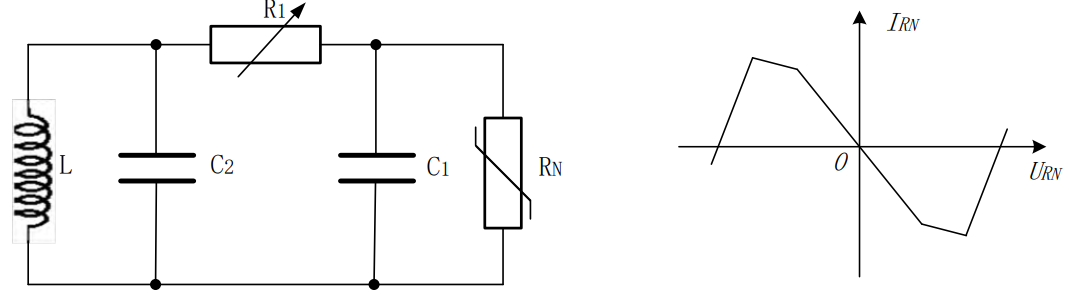
\includegraphics[width=0.7\textwidth]{attachments/fig.illus-1.1.png}
			}
			
			\subfloat[Chua's circuit I with two op-amps]{\label{fig.illus-1.2}
			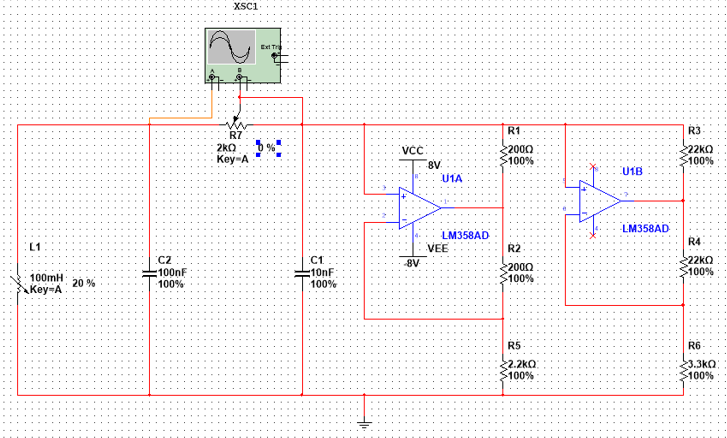
\includegraphics[width=0.45\textwidth]{attachments/fig.illus-1.2.png}
			}
			\subfloat[Chua's circuit II with one op-amp and two diodes]{\label{fig.illus-1.3}
			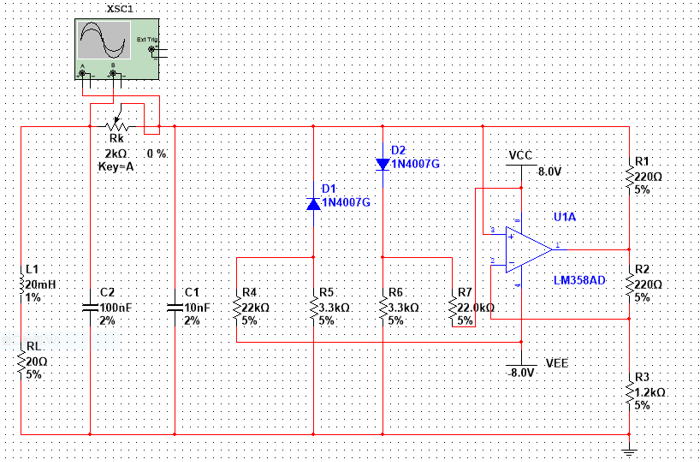
\includegraphics[width=0.45\textwidth]{attachments/fig.illus-1.3.png}
			}
			\caption{\textbf{The Chua's circuit}}
		\end{figure*}
	
		\subsubsection{Lorentz's circuit\autocite{lorenzDeterministicNonperiodicFlow1963}}
		\paragraph{A. The equation}~
		\newline 
		\indent
		The normalized Lorentz's equation is Eq. \ref{eq.2.1}
		\begin{align}
			&\left\{
				\begin{aligned}
					\frac{dx}{d \tau} &= -P(x-y) \\
					\frac{dy}{d \tau} &= \gamma x - y - xz \\
					\frac{dz}{d \tau} &= -bz +xy
				\end{aligned}
			\right. 
			\label{eq.2.1}
		\end{align}
		
		The equation, first derived by Lorentz in 1962 when dealing with the Benard convection experiment, 
		describe the atmospheric convection between two infinite planes\autocite{lorenzDeterministicNonperiodicFlow1963}, 
		where $x$ denotes the flip rate of convection, $y$ denotes the temperature difference between the rising and falling liquids during convection, 
		$z$ denotes the temperature gradient in the vertical direction. 
		Obviously, $xy$ and $xz$ are two nonlinear terms. 
		
		($P, \gamma, b$) are dimensionless parameters, where $P$ is the Prandtl number, which is proportional to the diffusion coefficient of the liquid. 
		$b$ is the velocity damping constant and is related to the size of the convection current.
		$\gamma = \frac{R}{R_C}$ is called the relative Rayleigh number and describes the properties of fluid motion . 
		If $R > R_C$, i.e. $\gamma > 1$, convection will occur. If $\gamma$ is even greater, chaotic phenomena such as torrents will appear.

		Lorentz found that if the initial parameters ($P, \gamma, b$) were set as ($P=10, \gamma=28, b=\frac{8}{3}$),
		the system would present a chaotic pattern called the "Lorentz butterfly".

		This equation can be easily implemented in an analog electronic circuit, as shown below.

		\paragraph{B. The circuit}~
		\newline 
		\indent
		The Lorentz's circuit(Fig. \ref{fig.illus-2.1}) used in this study was developed by Paul Horowitz at Harvard University, 
		and the circuit is accessible on his website (\href{http://seti.harvard.edu/unusual_stuff/misc/lorenz.htm}{http://seti.harvard.edu}). 
		Horowitz built this circuit with just 3 op-amps (each does both an integration and a sum) and two analog multipliers (to form the products xy and xz), 
		and the op-amps are wired as integrators, with the various terms that make up each derivative summed at the inputs.
		\begin{figure*}[htbp]
			\centering
			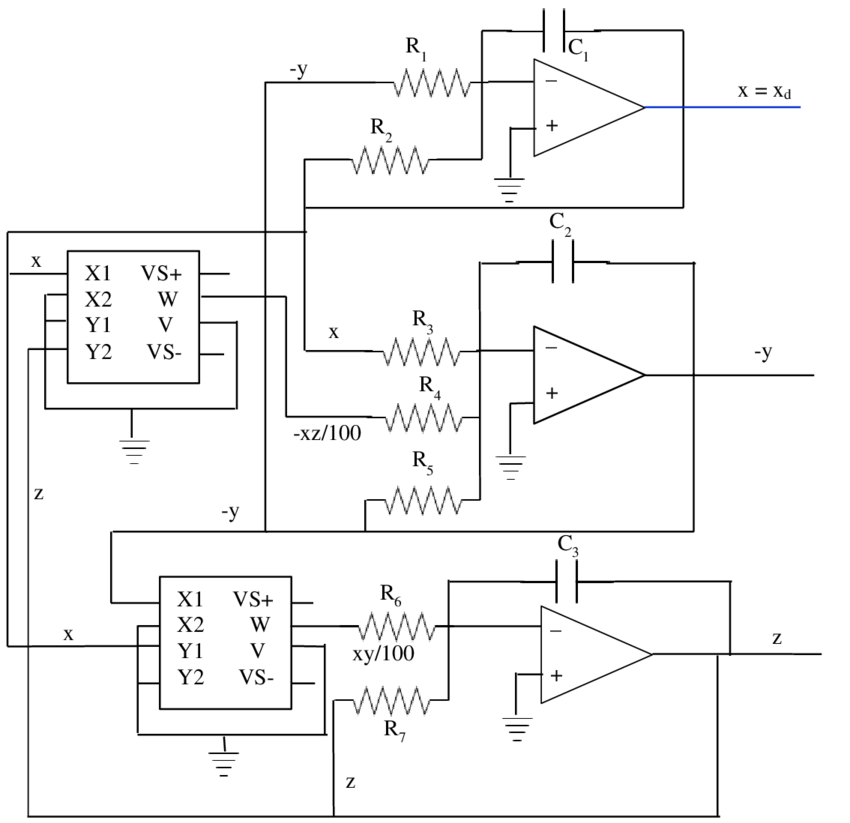
\includegraphics[width=0.4\textwidth]{attachments/fig.illus-2.1.png}
			\caption{\textbf{The Lorentz's circuit}}
			\label{fig.illus-2.1}
		\end{figure*}
	\subsection{Major instruments and materials}

		\paragraph{A. Anaconda} Computation environment to perform numerical calculations.
		\paragraph{B. Multisim and LTspice} SPICE environment that lets users prototype, design, and test electrical circuits in a simulated manner.
		\paragraph{C. NI VitualBench} NI VirtualBench is an all-in-one instrument that combines a mixed signal oscilloscope with protocol analysis, an arbitrary waveform generator, a digital multimeter, and so on. 
		In this experiment we use this instrument to obtain the oscillation patterns of chaotic circuits.

		Details are provided in the Supplementary Information.
	\subsection{Method}
		
		For Chua's circuit, we first did the numerical calculation for Eq. \ref{eq.1.1} to obtain all the five oscillation patterns and their initial parameters, respectively. 
		Then, on the basis of these parameters, we built the simulation circuits and adjusted the resistance value of $R_1$ to obtain different oscillation patterns. 
		Both circuits introduced previously (Fig. \ref{fig.illus-1.2} and Fig. \ref{fig.illus-1.3}) were tested.
		Finally, we built real-world circuits for both and, the same, adjusted the resistance value of $R_1$ to obtain different oscillation patterns.

		For Lorentz's circuits we only conducted the numerical calculation and simulation experiment to obtain the "Lorentz butterfly".
		Due to the lack of necessary components, we were unable to build the real-world circuit model.

%%end-------------------Method-----------------------%%

%%begin-------------------Result-----------------------%%
\section{Result}
	\subsection{Chua's circuit}
		\subsubsection{Numerical calculation}
			
			Different numerical solutions of chaotic oscillations were obtained by solving Eq. \ref{eq.1.1} with different parameters $\alpha, \beta, m_1, m_2$.
			Five typical chaotic oscillation patterns including 
			straight line(Fig. \ref{fig.1.1}), limit ring(Fig. \ref{fig.1.2}), double attractors(Fig. \ref{fig.1.3}), the first single attractor(Fig. \ref{fig.1.4}), and the second single attractor(Fig. \ref{fig.1.5}) 
			were observed.

			The parameters of different chaotic oscillation patterns are summarized in the Supplementary Information.
	
			A Jupyter Notebook including all codes for calculation and an interactive ipywidget which allows adjusting the parameters conveniently is available on \href{https://github.com/Zweig-Wong/SYSU-PHY-EXP/blob/main/C9-Chaotic_circuit/Chua/Calculation/Chua.ipynb}{https://github.com/Zweig-Wong/SYSU-PHY-EXP} 
			\begin{figure*}[htbp]
				\centering
				\subfloat[Channel]{
				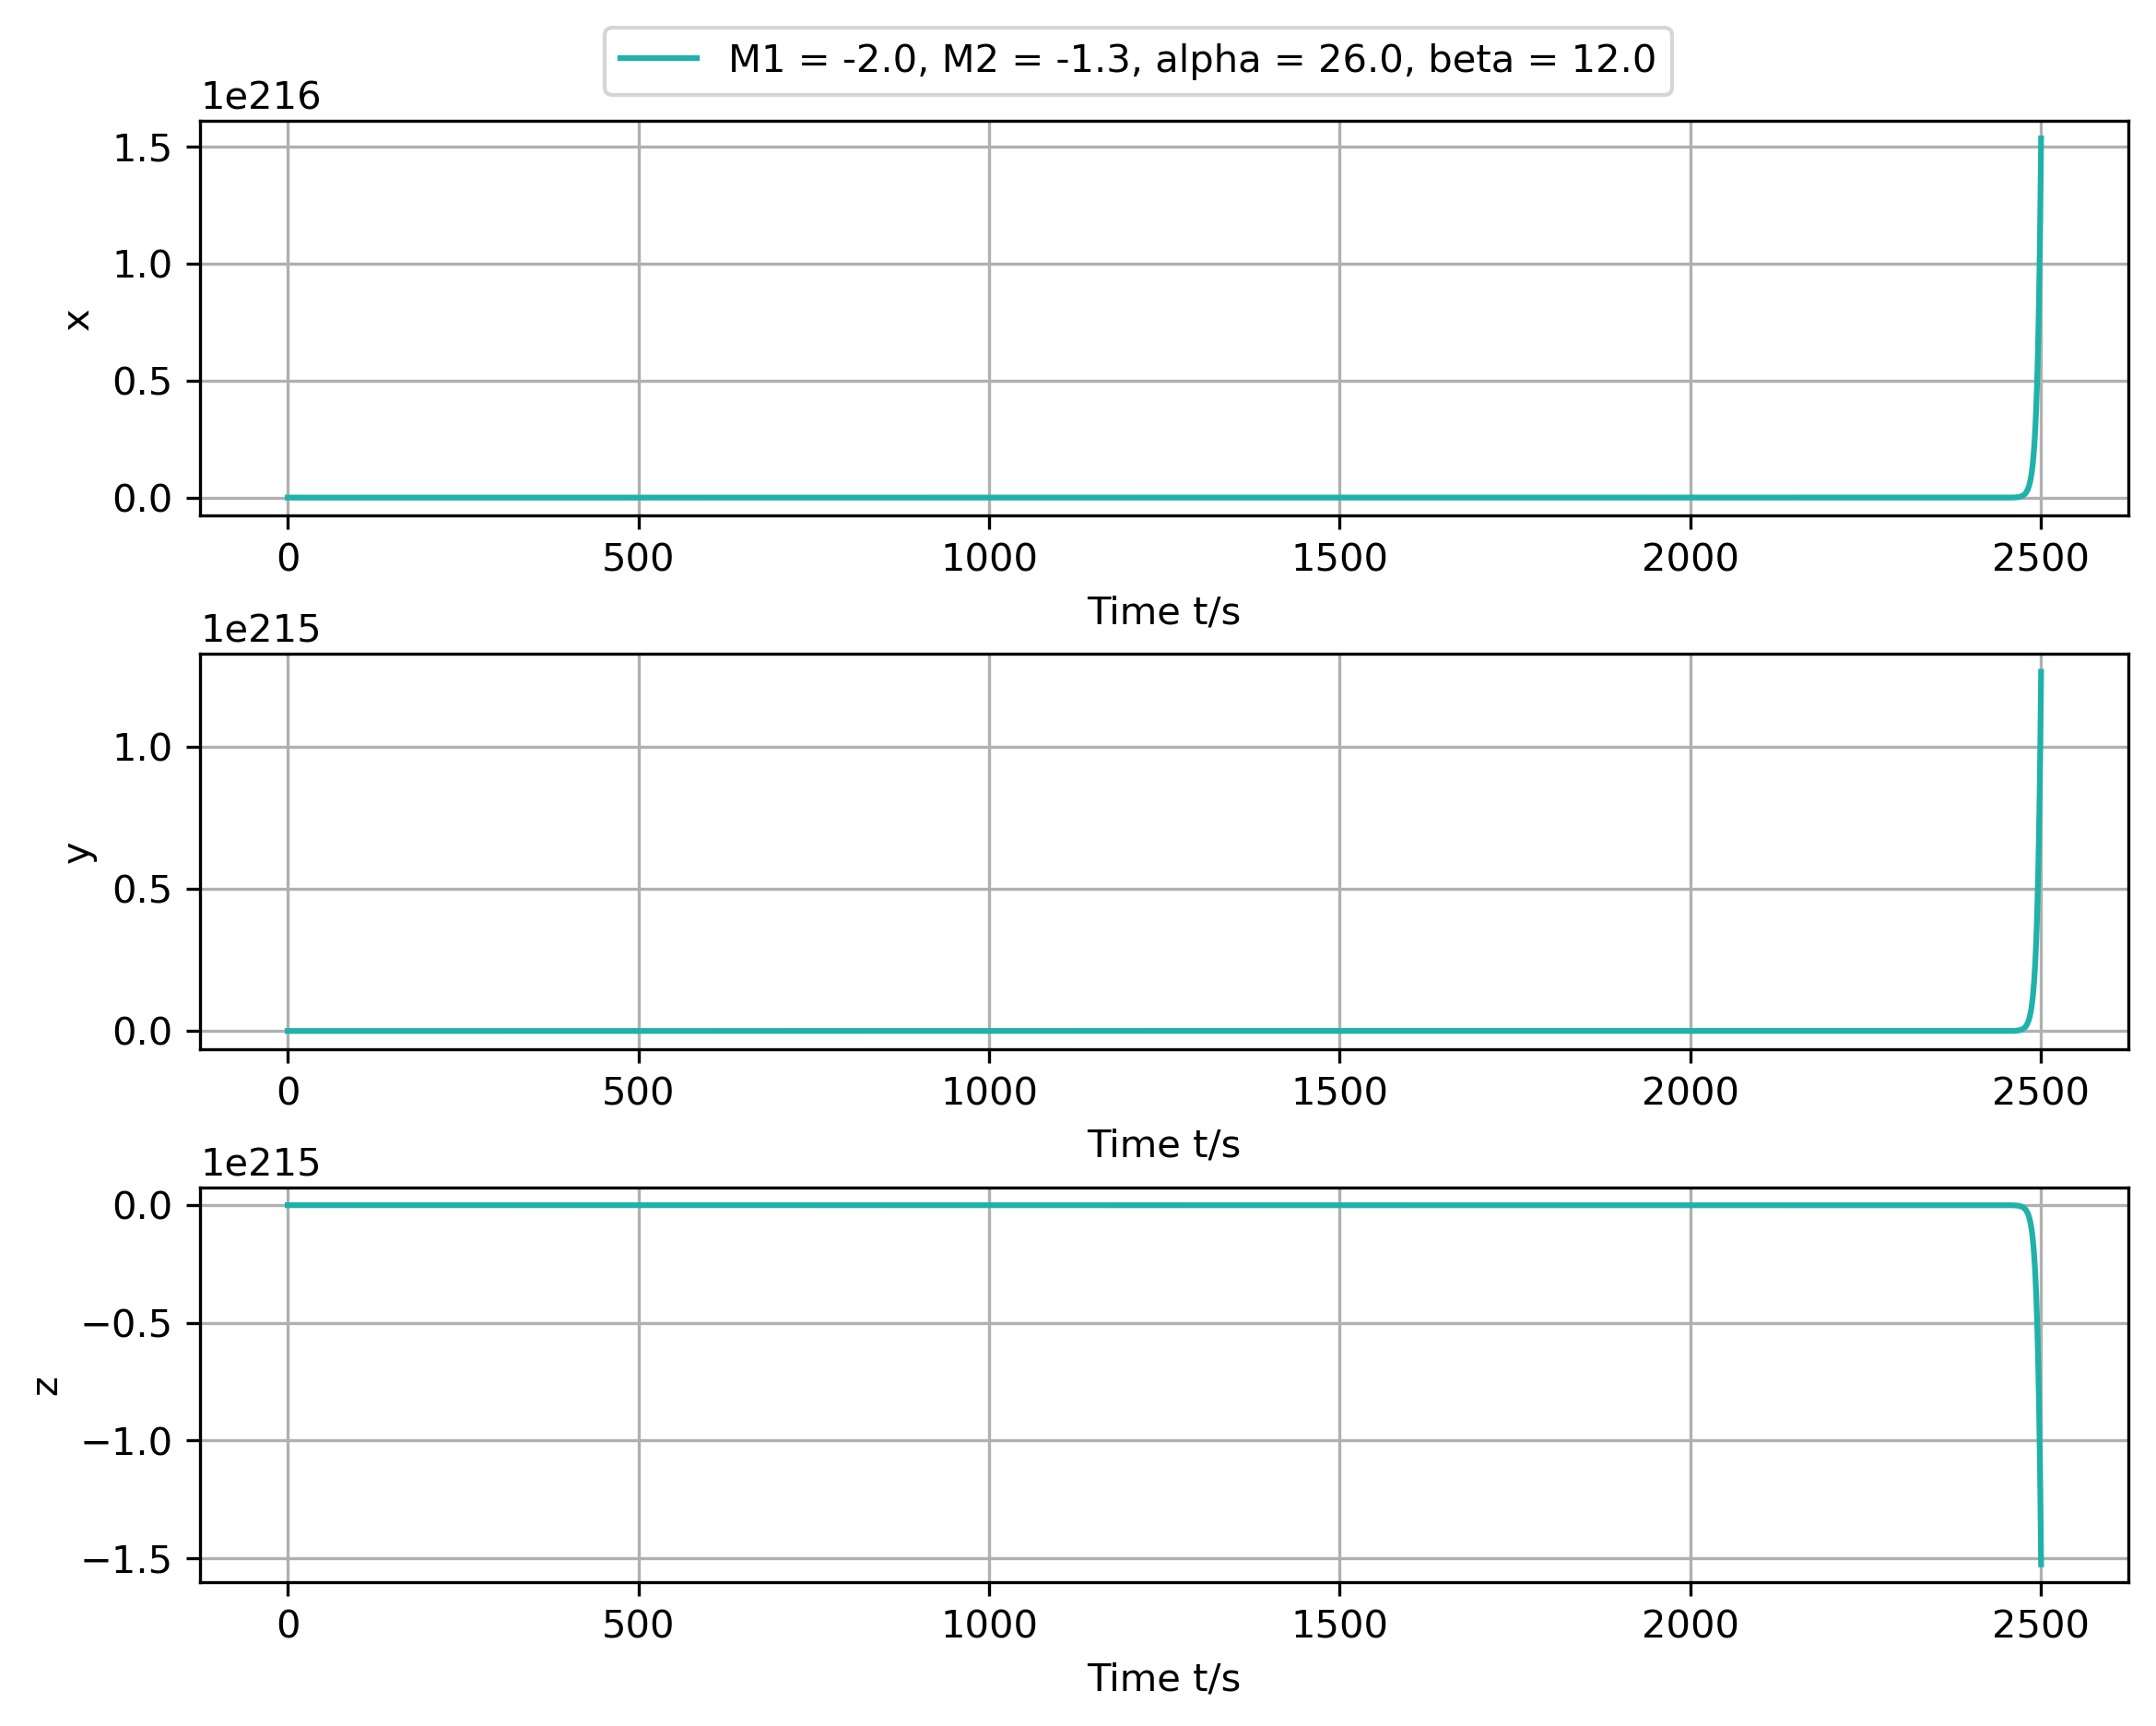
\includegraphics[width=0.3\textwidth]{attachments/fig.1.1.wave.png}
				}
				\subfloat[3d trace]{
				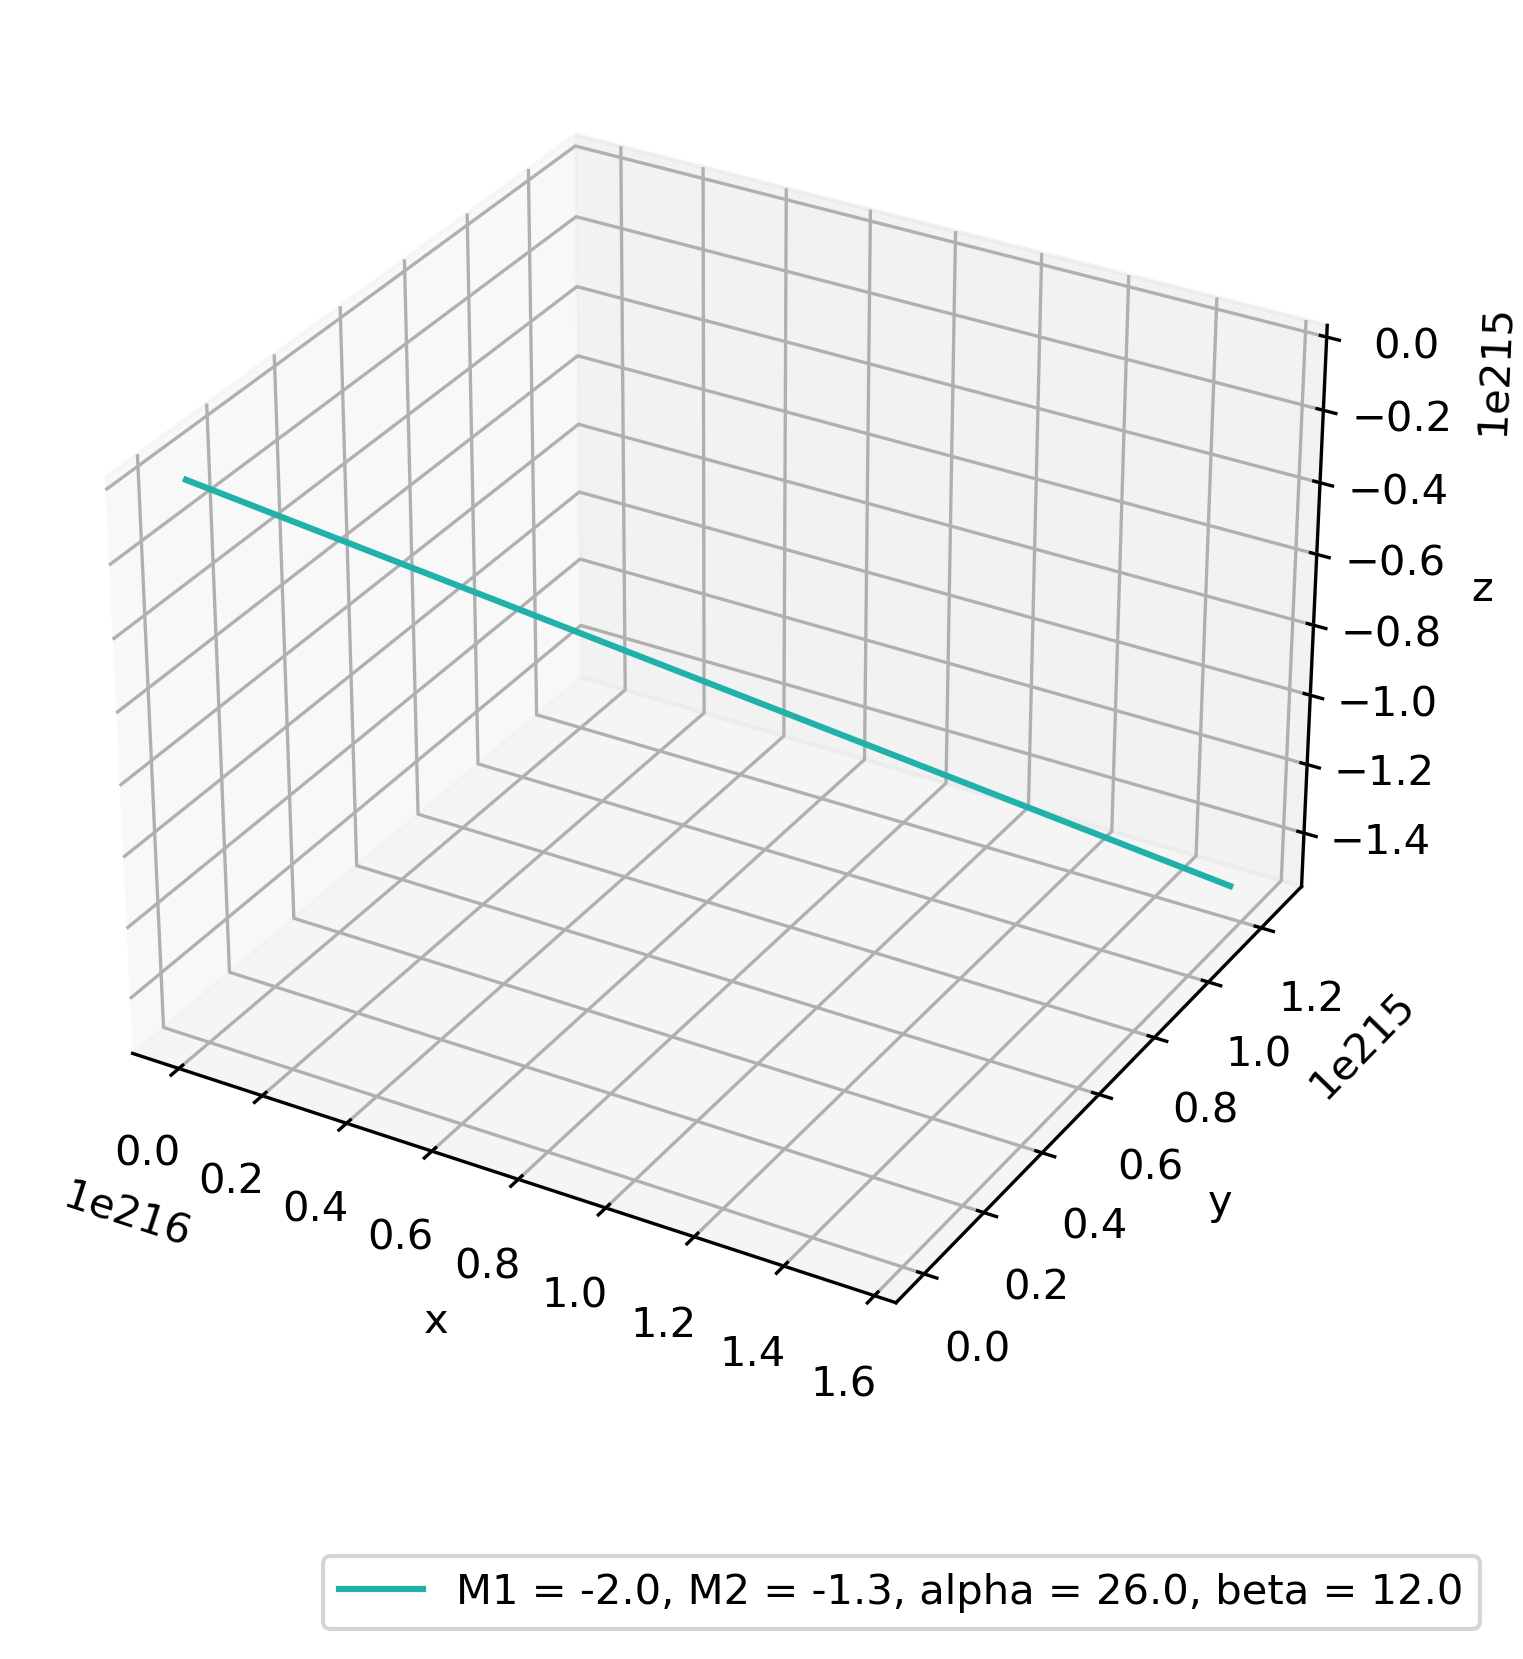
\includegraphics[width=0.3\textwidth]{attachments/fig.1.1.3d.png}
				}
				
				\subfloat[x-y plain]{
				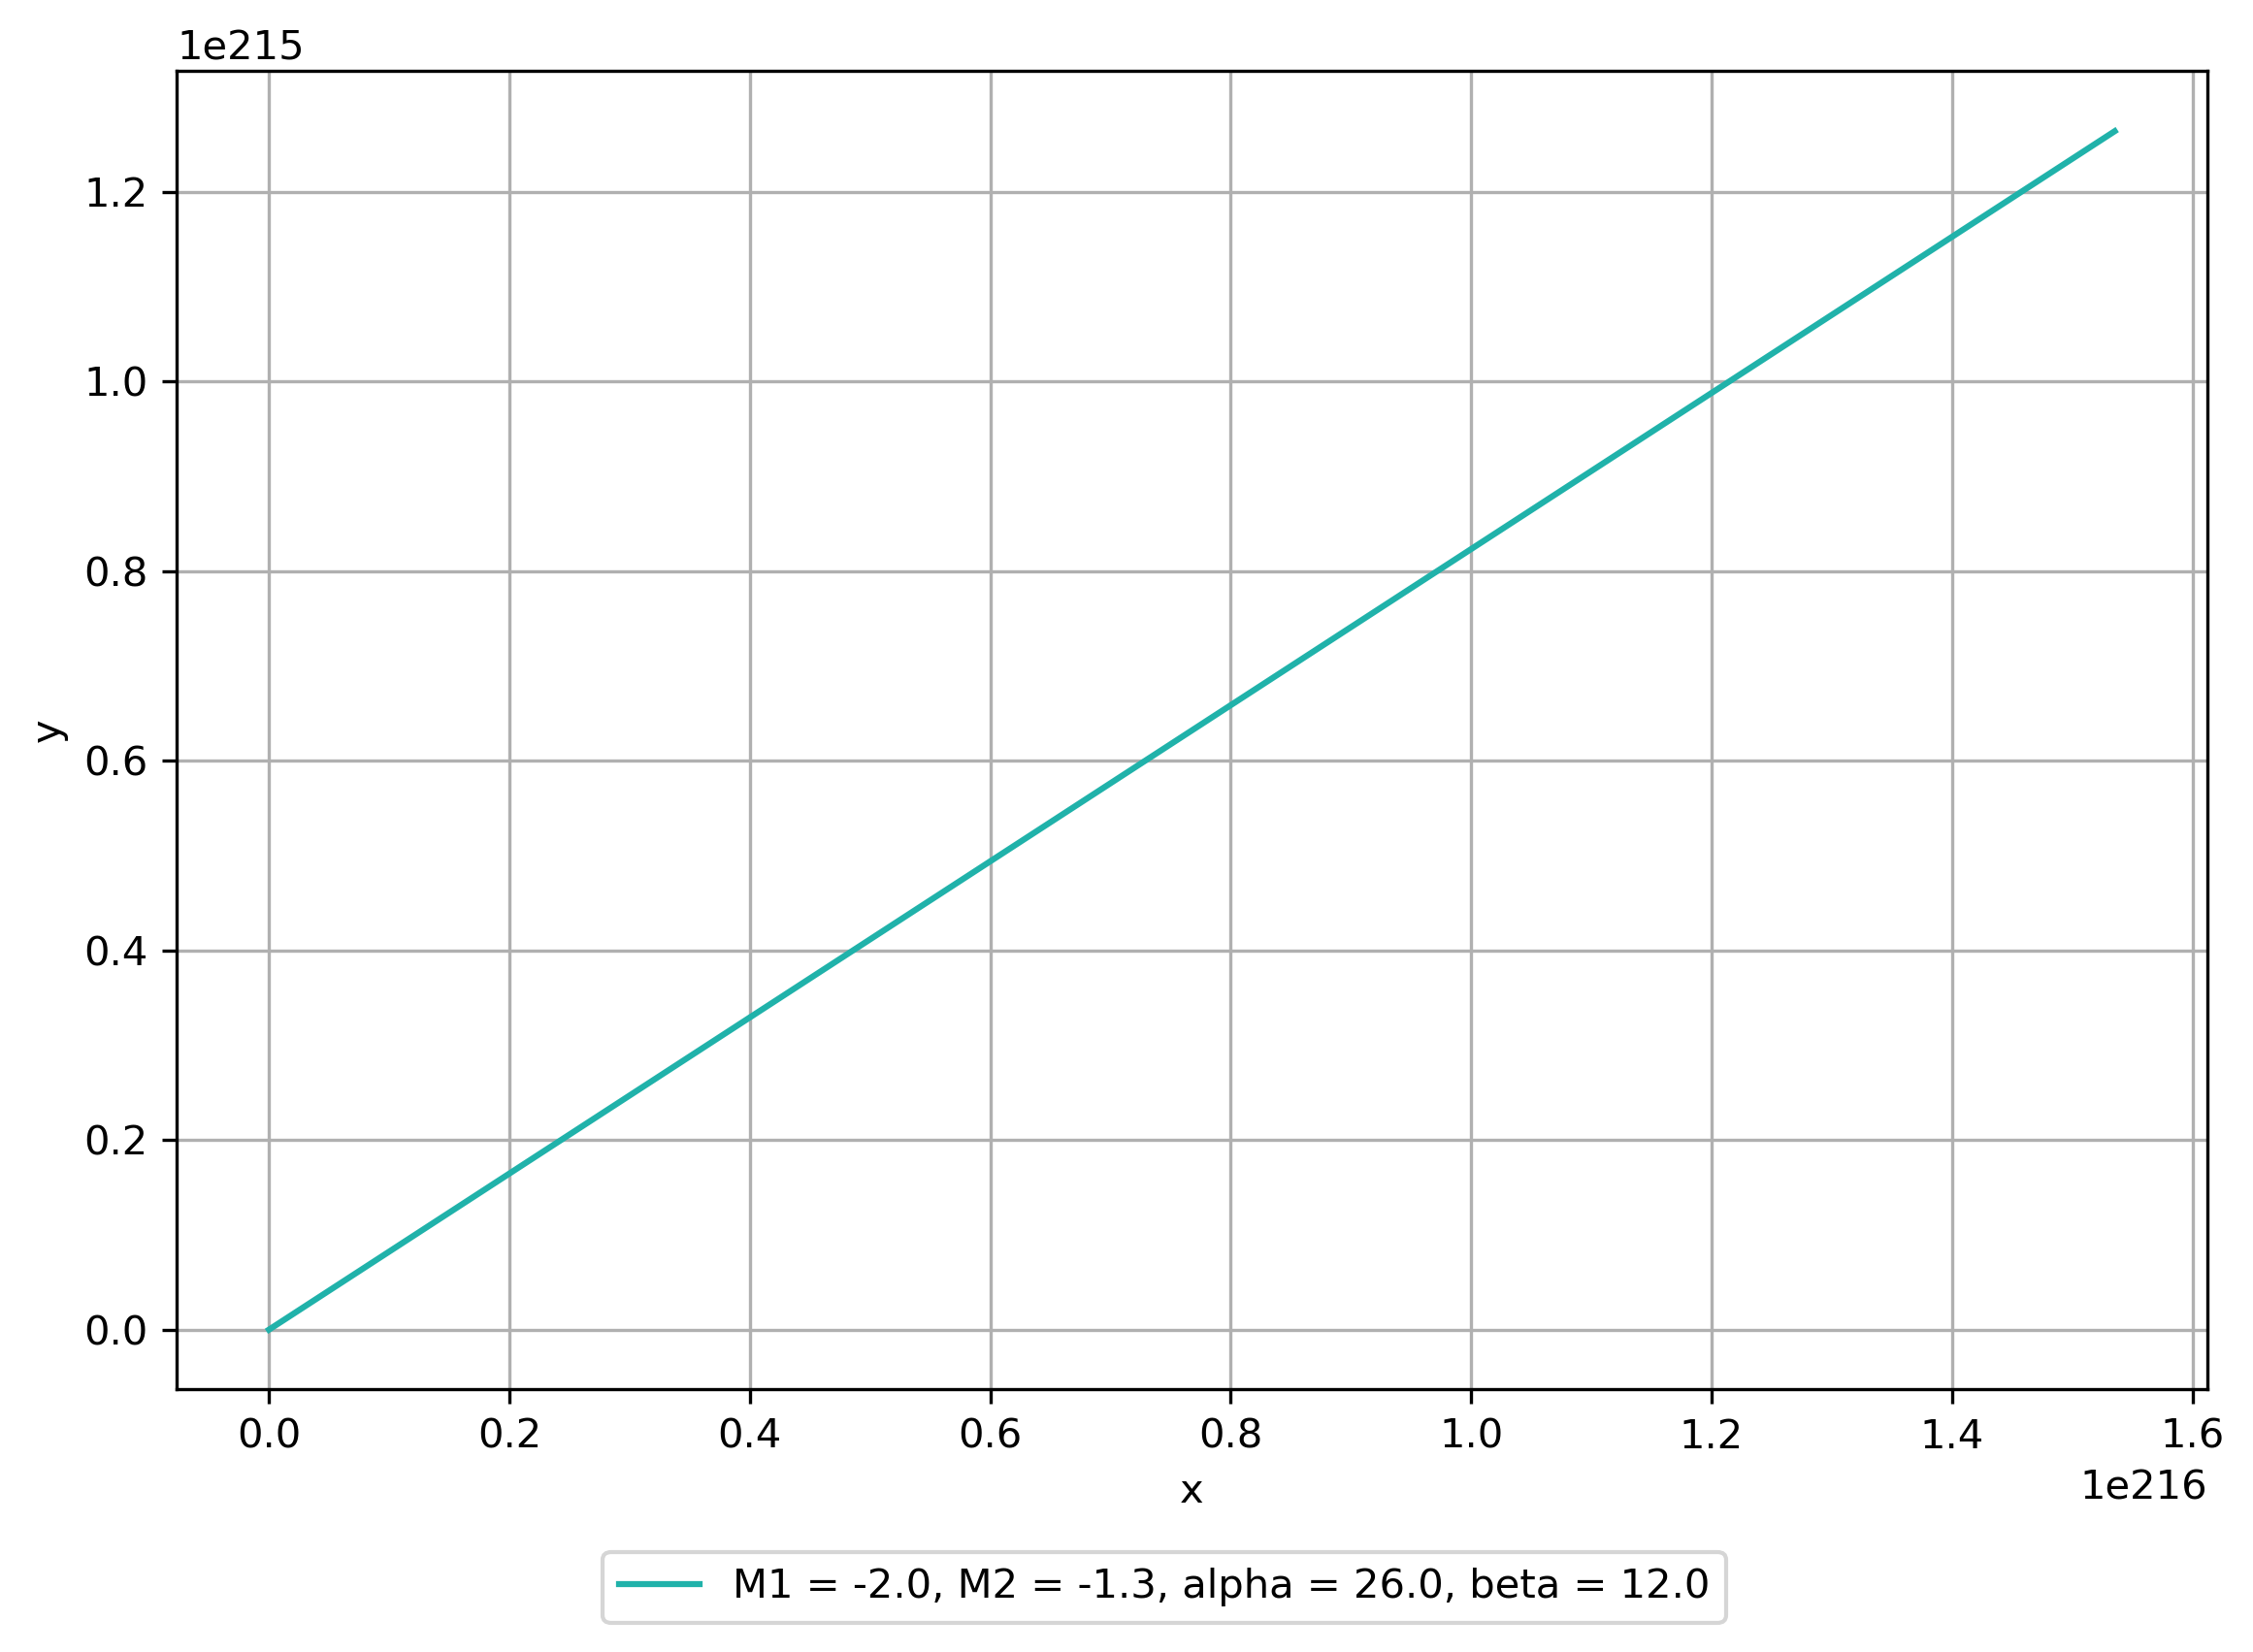
\includegraphics[width=0.3\textwidth]{attachments/fig.1.1.x-y.png}
				}
				\subfloat[x-z plain]{
				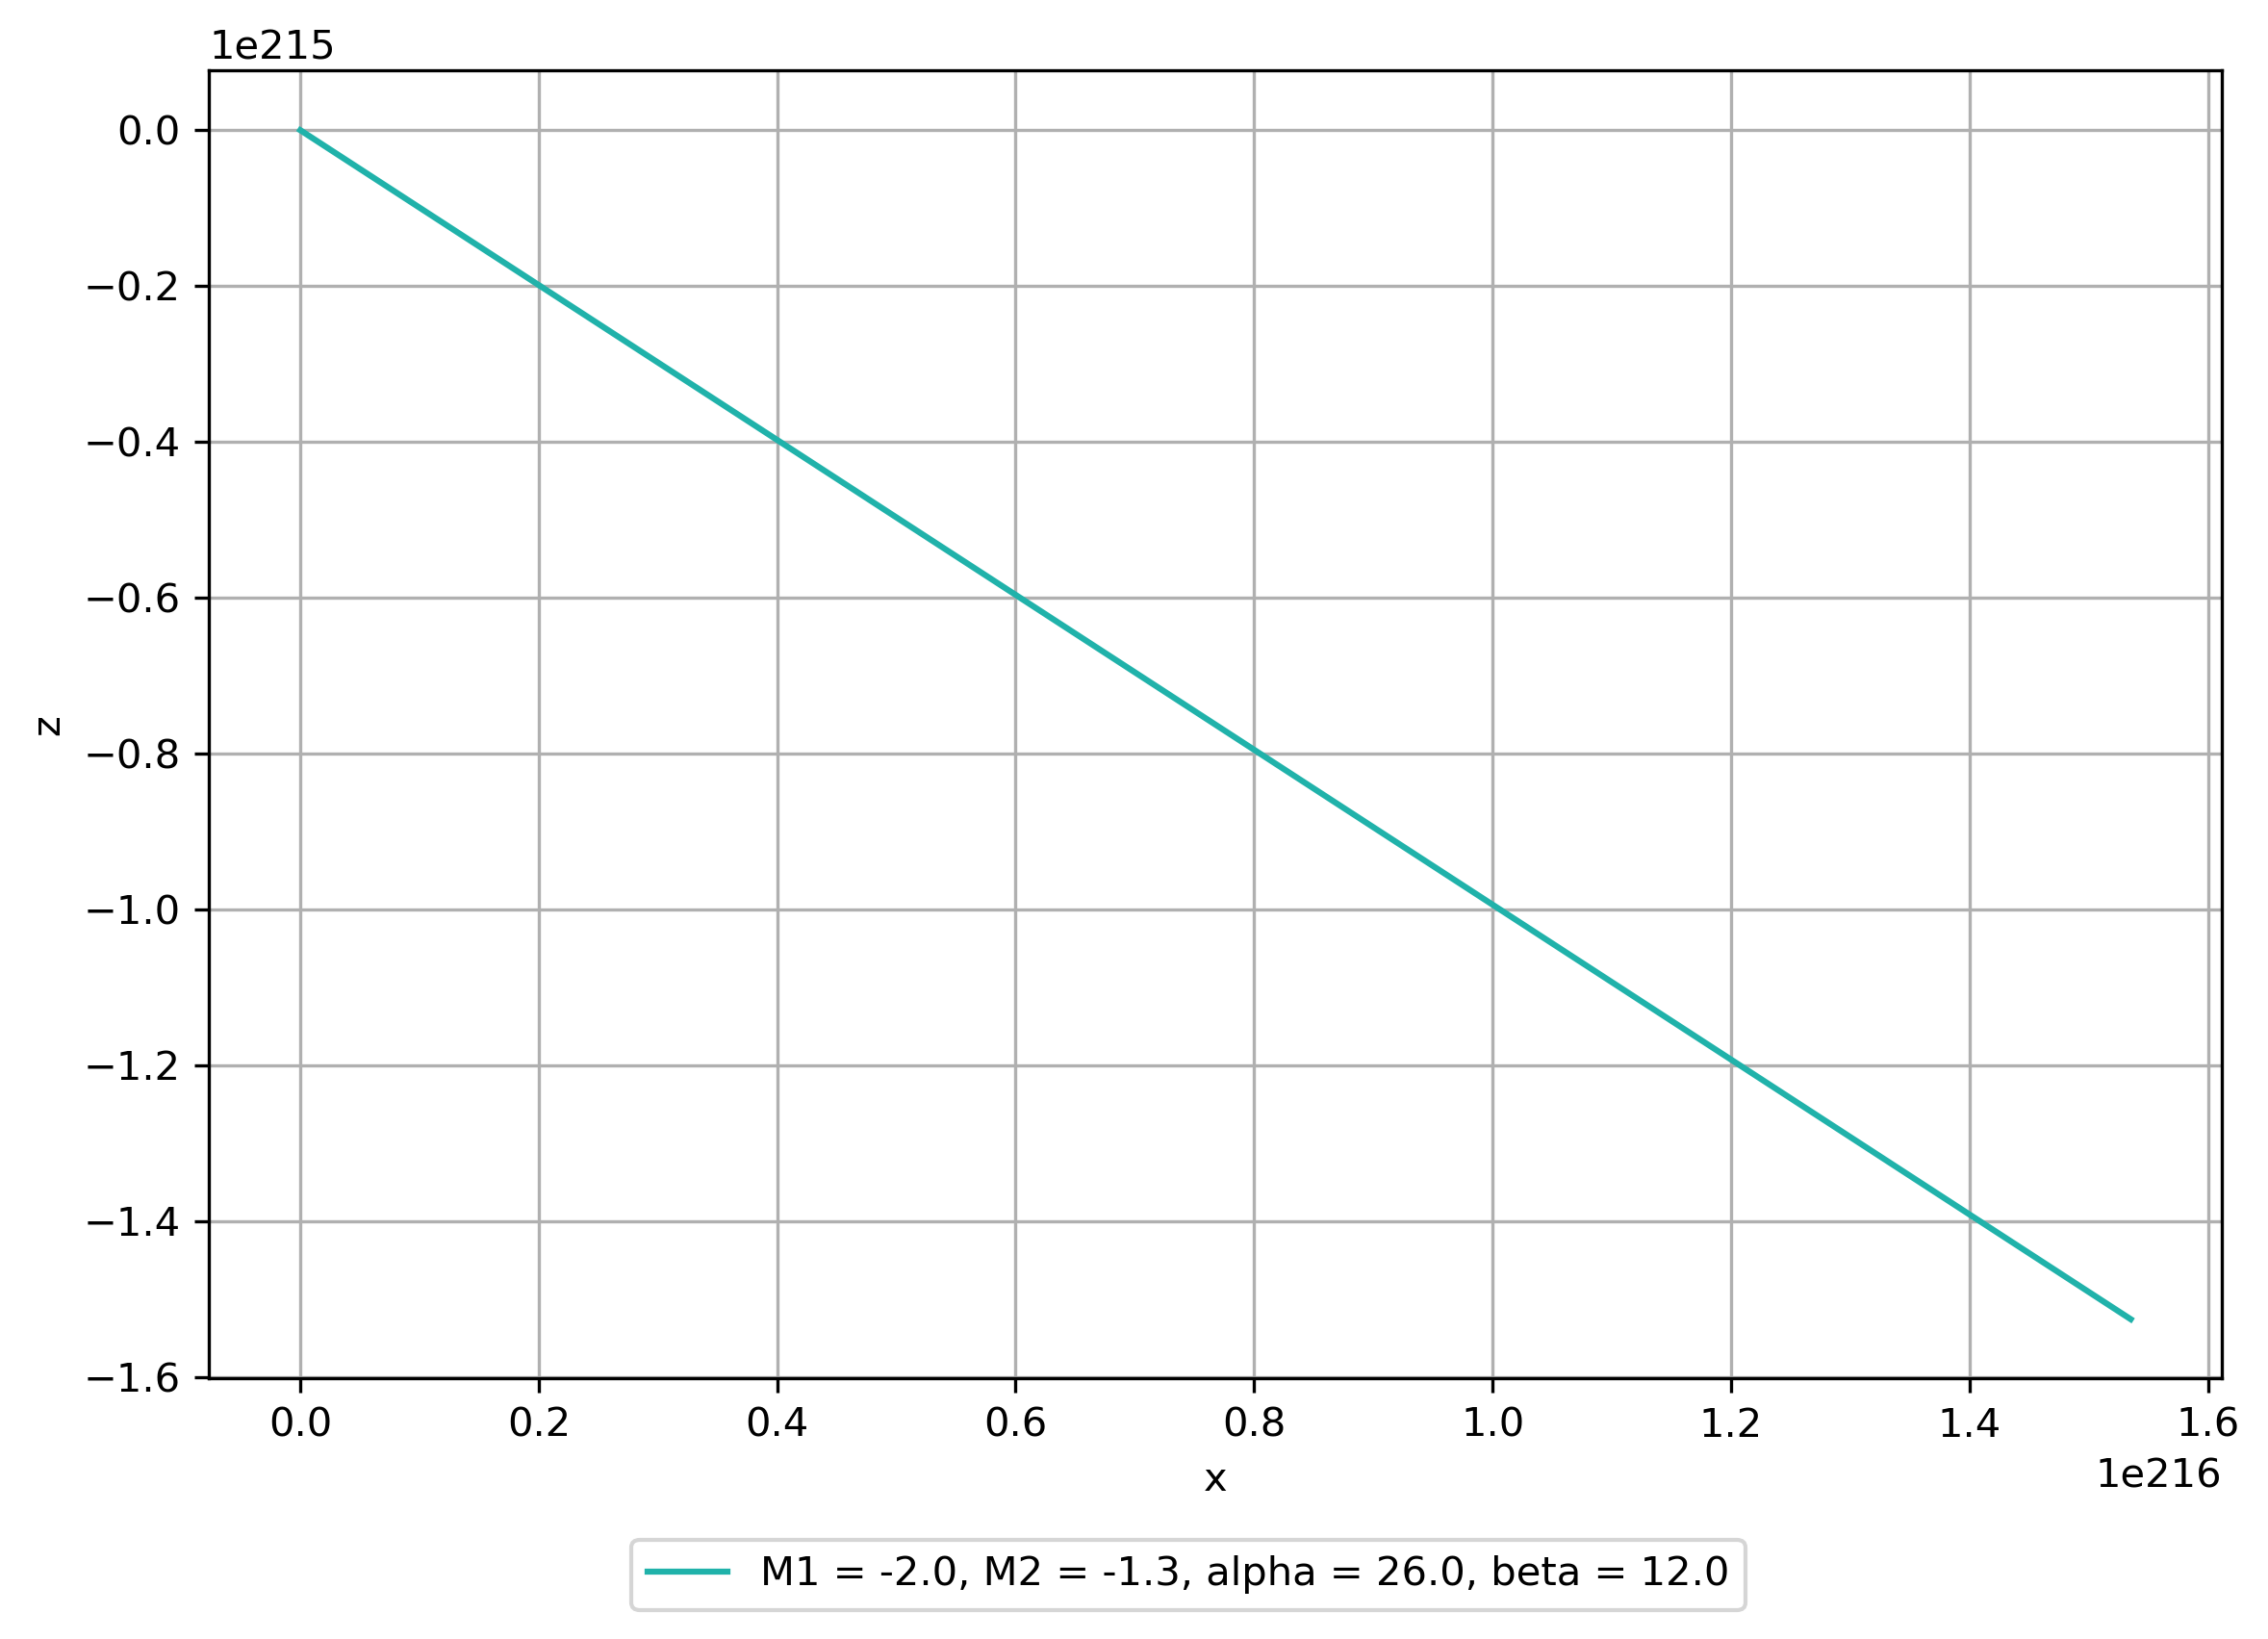
\includegraphics[width=0.3\textwidth]{attachments/fig.1.1.x-z.png}
				}
				\subfloat[y-z plain]{
				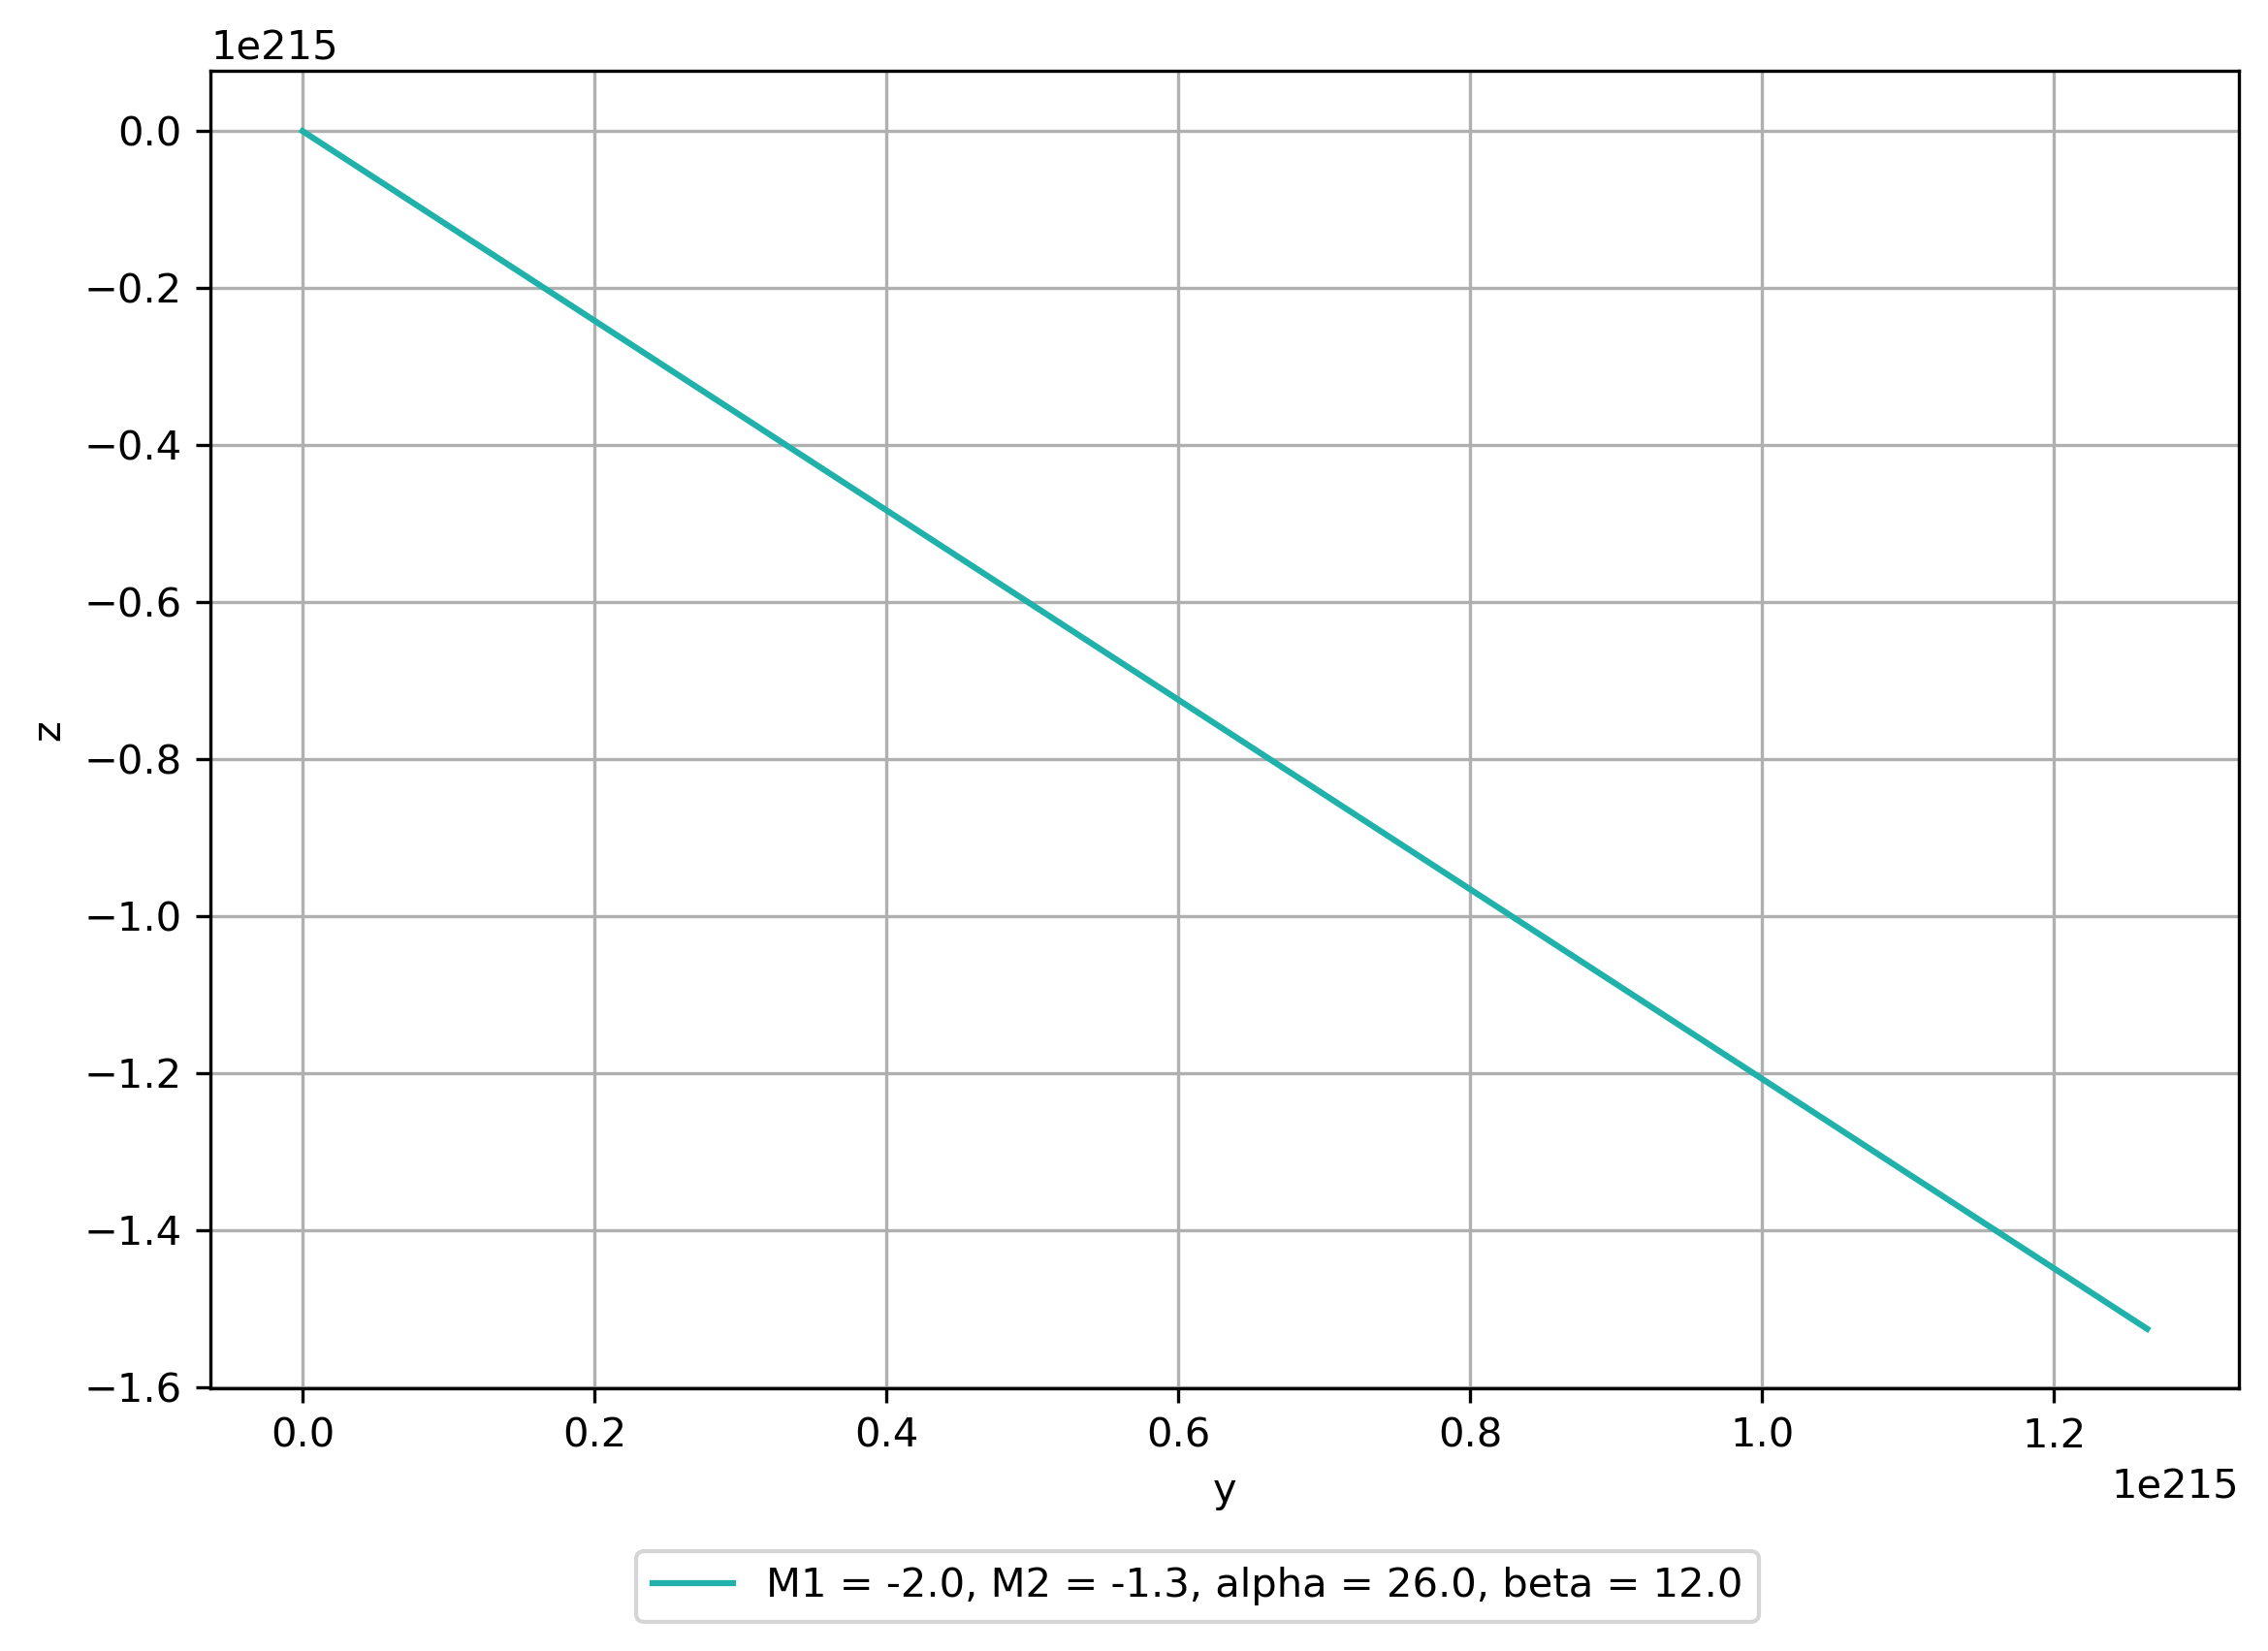
\includegraphics[width=0.3\textwidth]{attachments/fig.1.1.y-z.png}
				}
				\caption{\textbf{Numerical calculation of Chua's circuit, line}}
				\label{fig.1.1}
			\end{figure*}
			
			\begin{figure*}[htbp]
				\centering
				\subfloat[Channel]{
				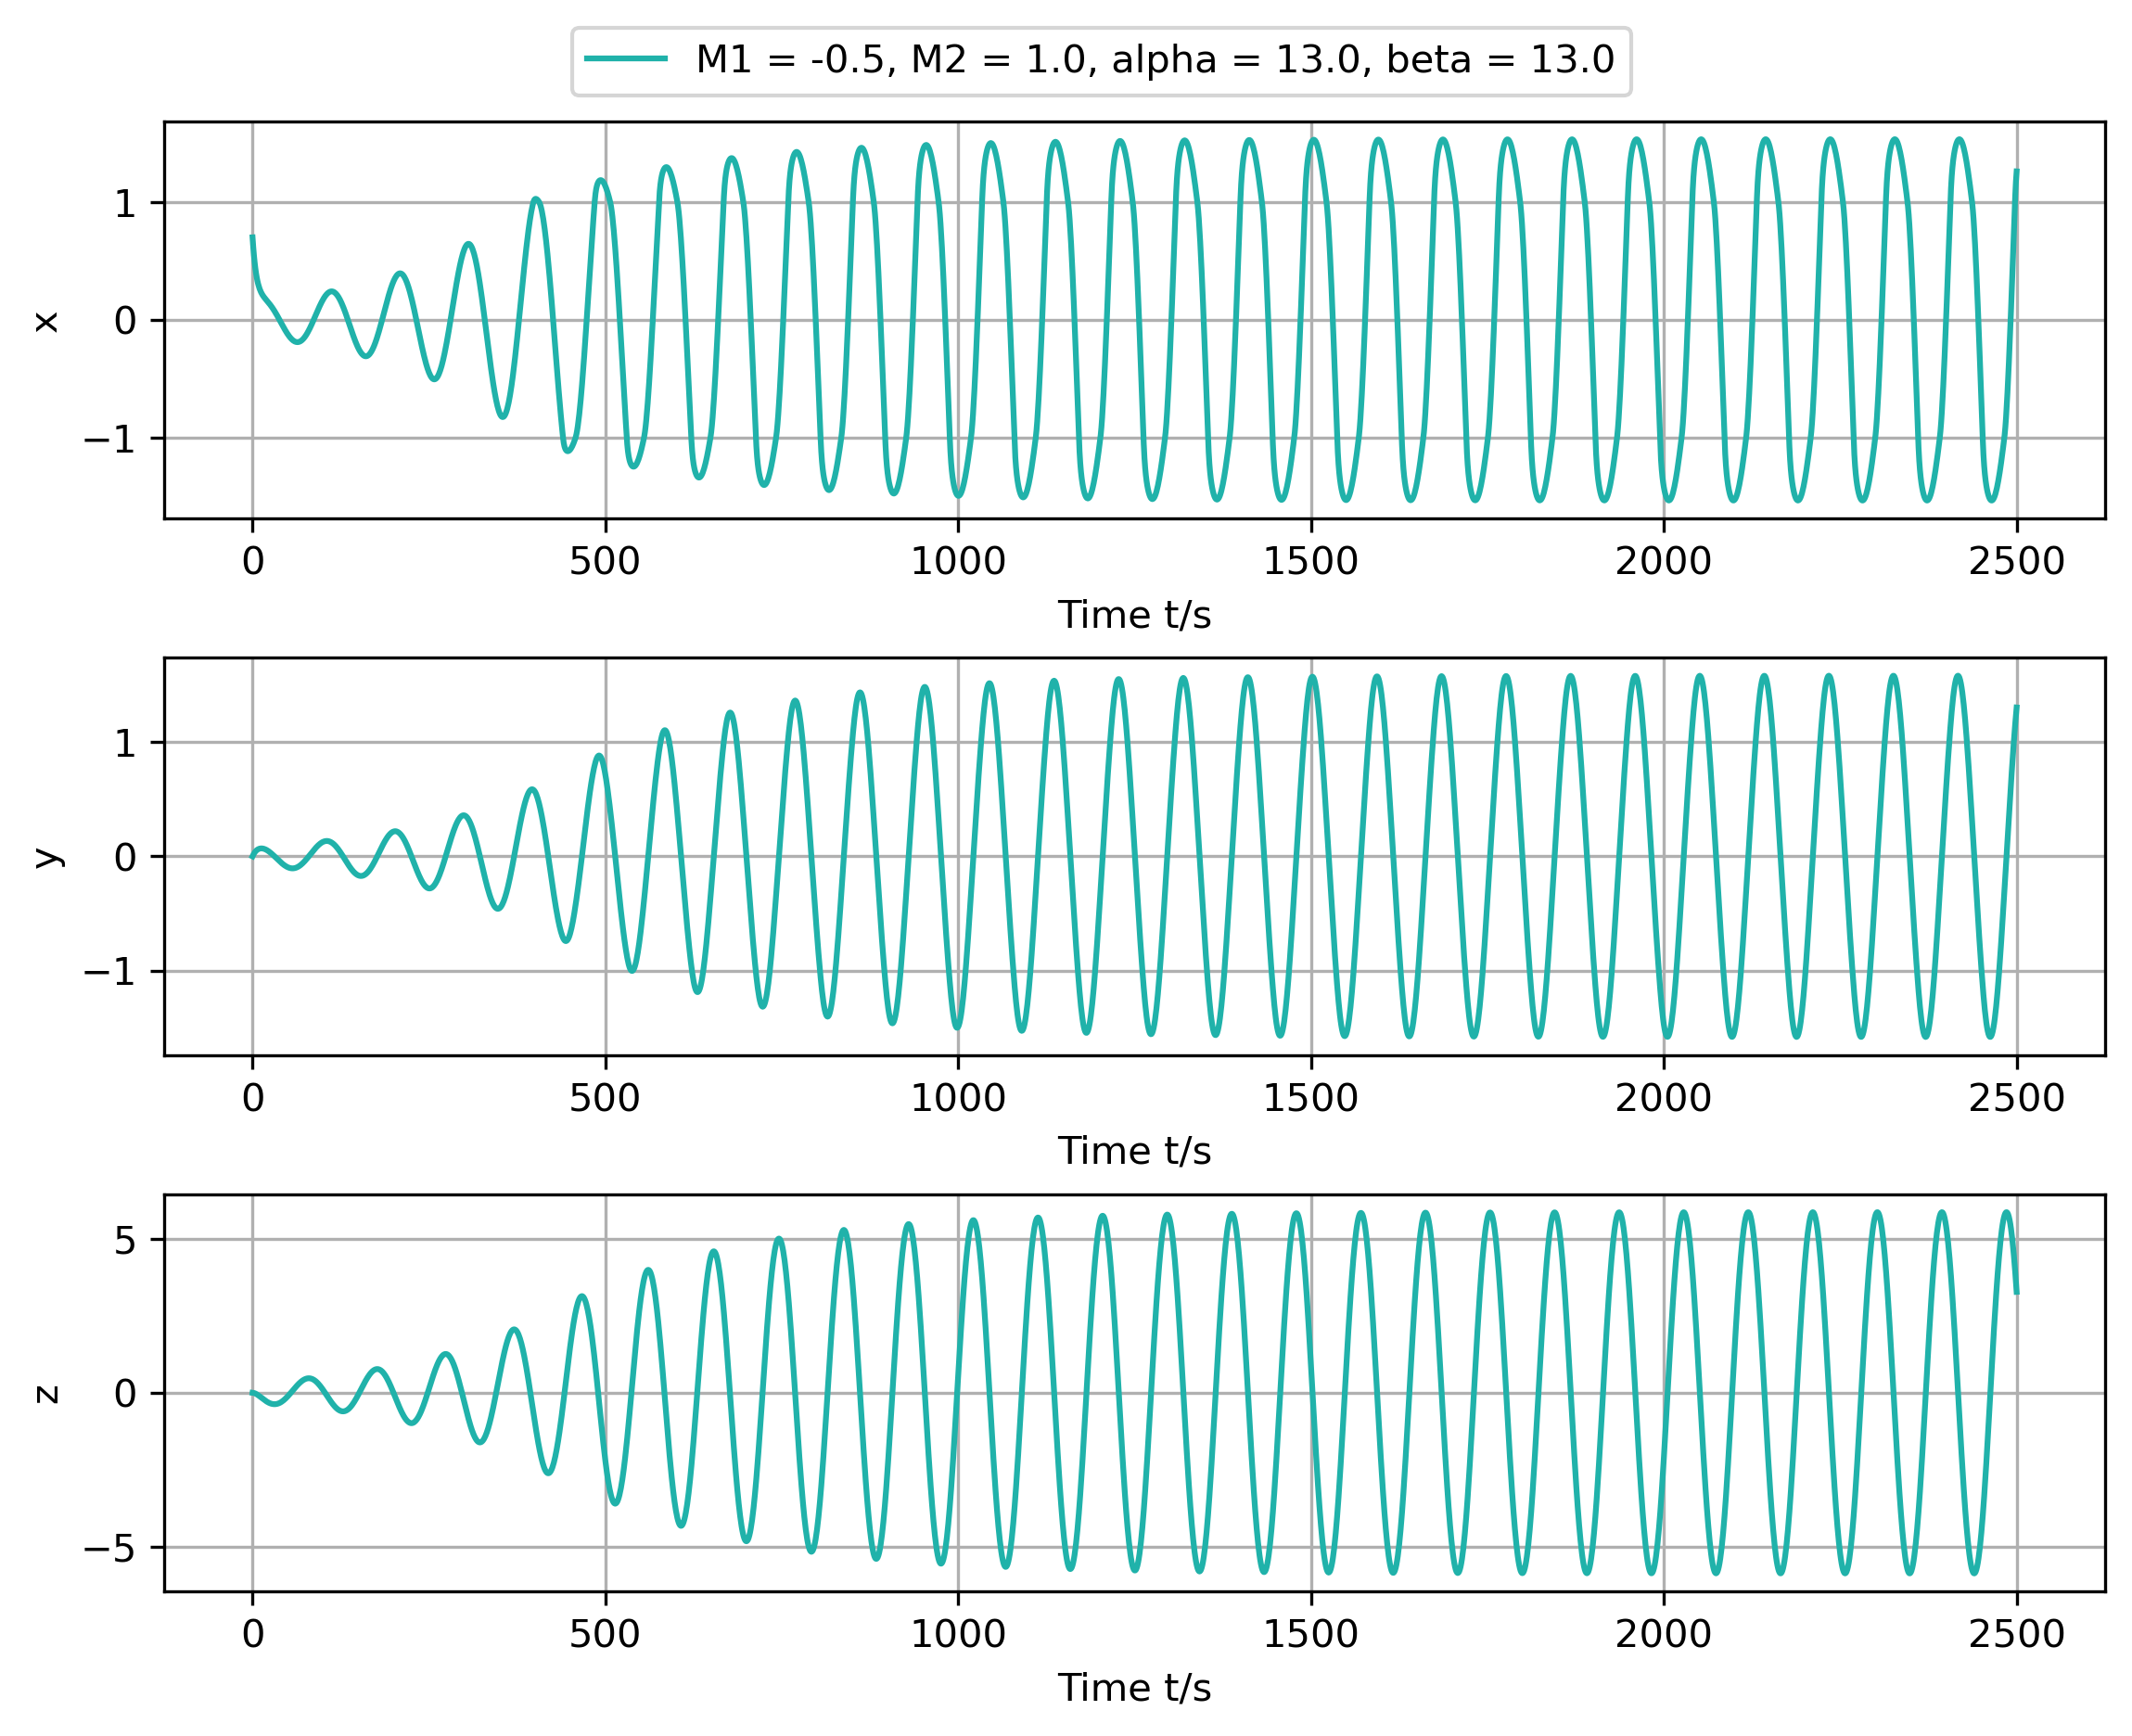
\includegraphics[width=0.3\textwidth]{attachments/fig.1.2.wave.png}
				}
				\subfloat[3d trace]{
				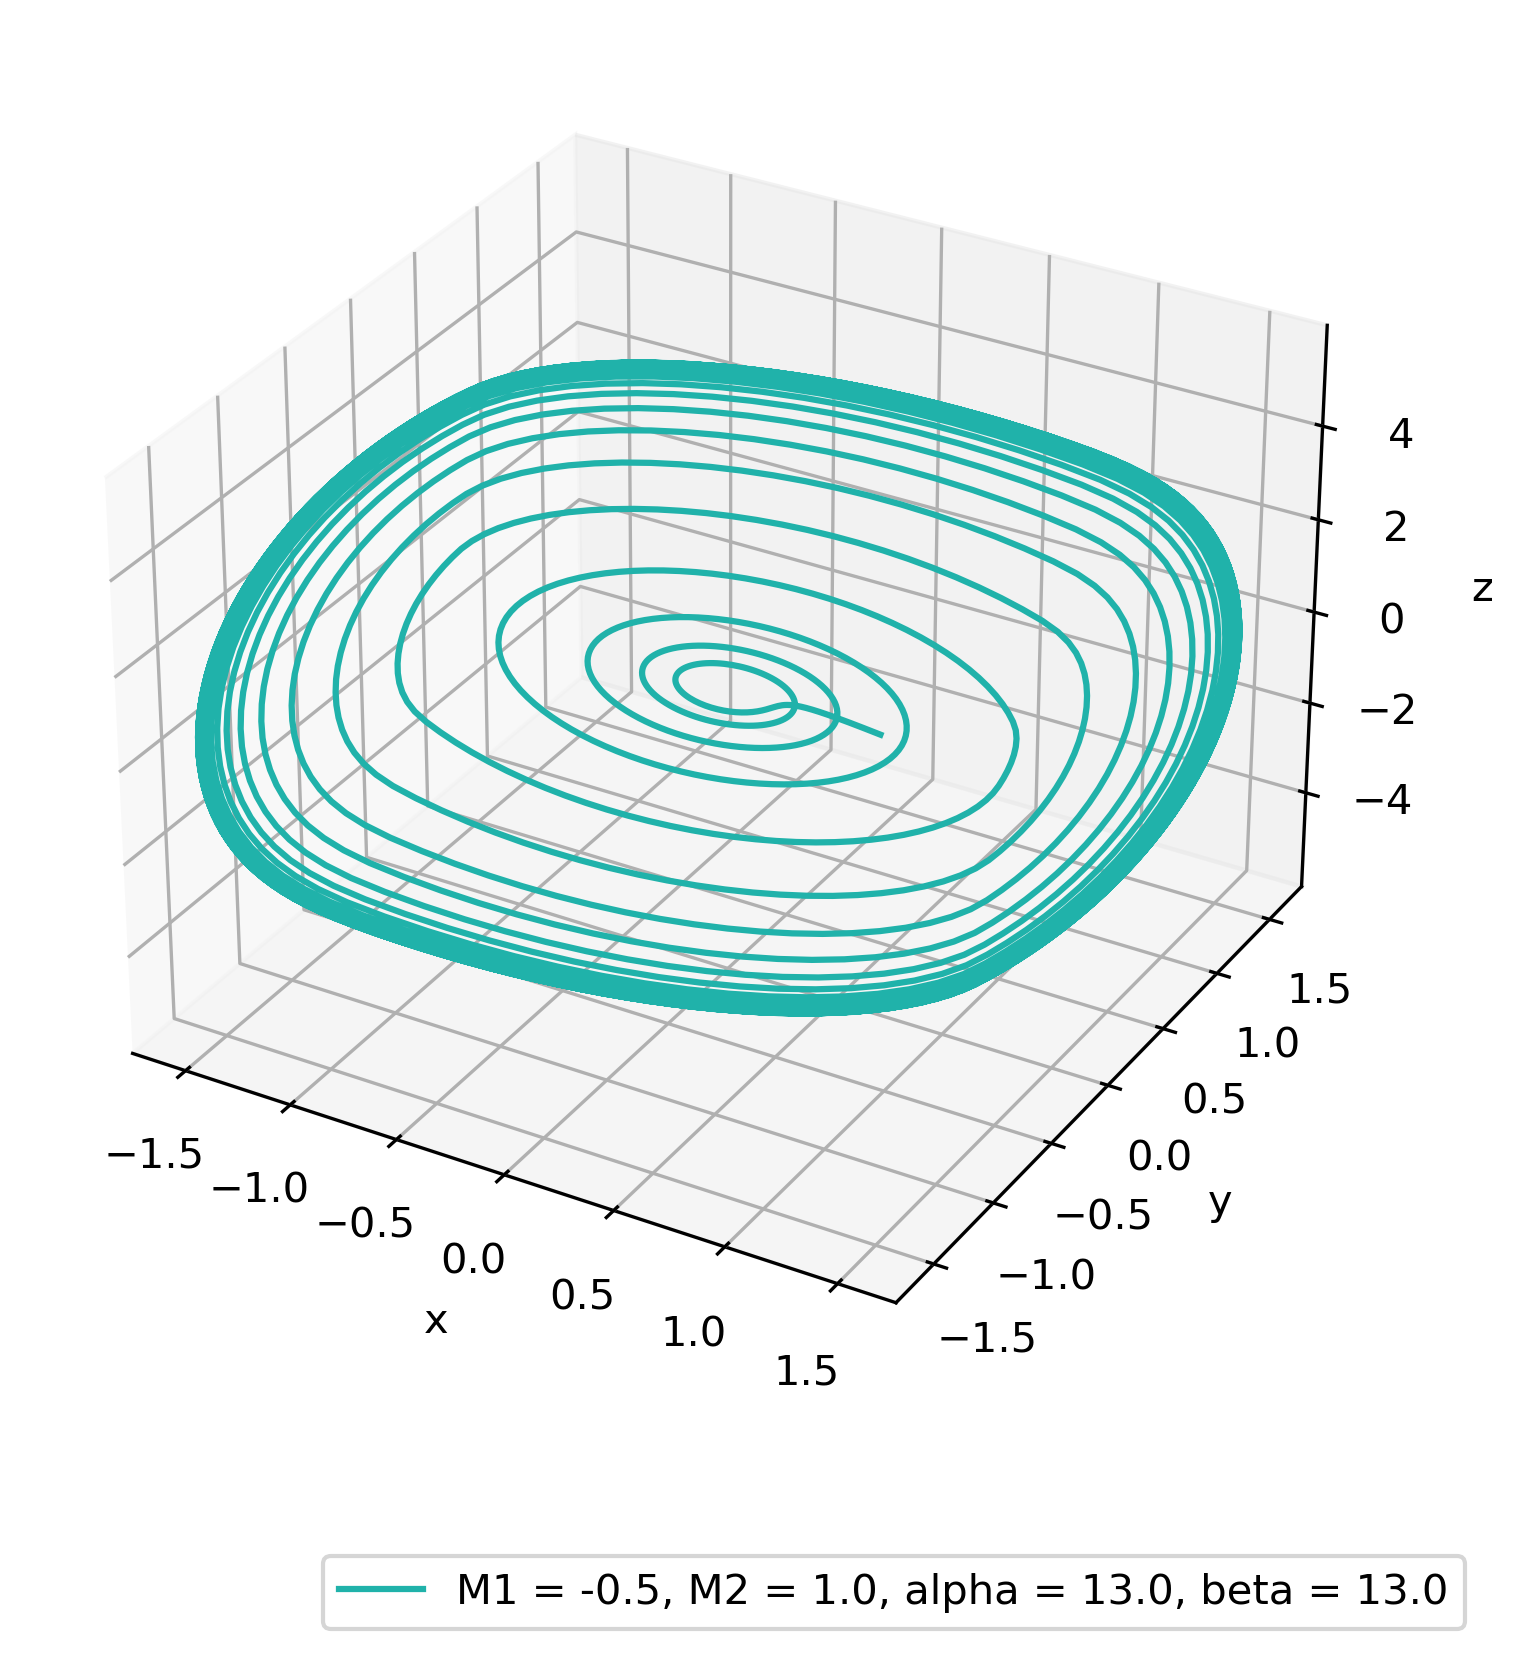
\includegraphics[width=0.3\textwidth]{attachments/fig.1.2.3d.png}
				}

				\subfloat[x-y plain]{
				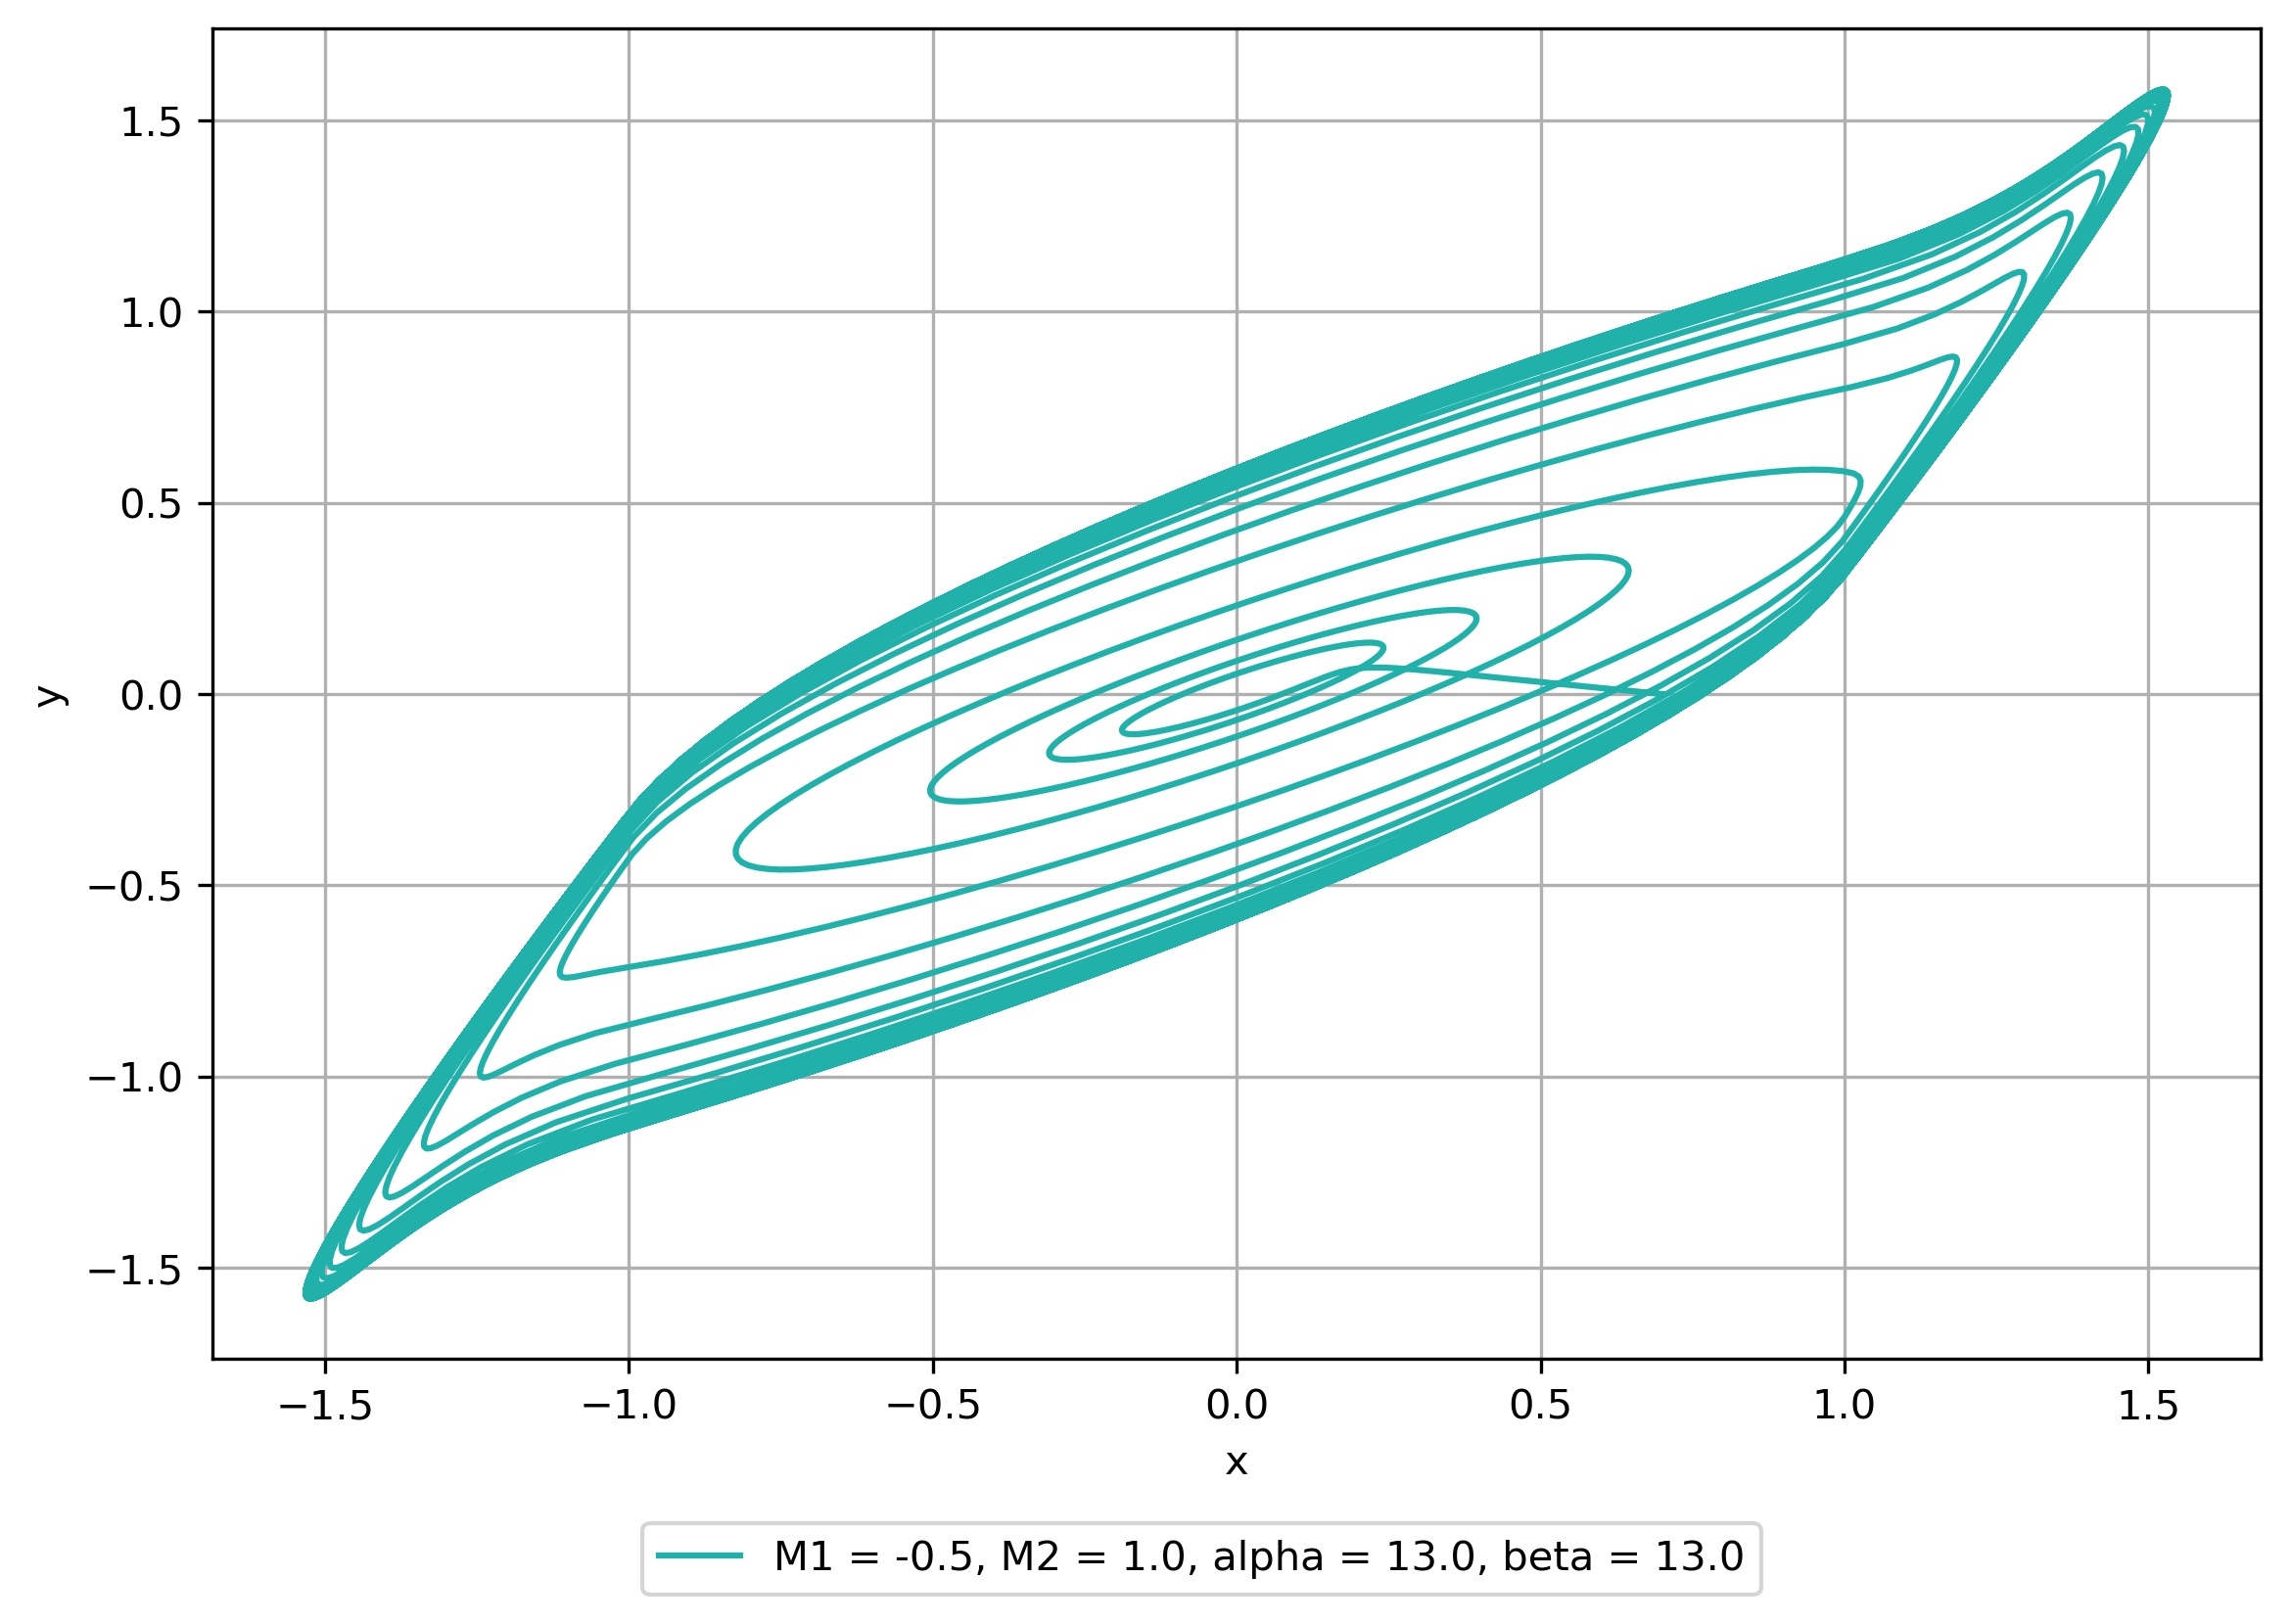
\includegraphics[width=0.3\textwidth]{attachments/fig.1.2.x-y.png}
				}
				\subfloat[x-z plain]{
				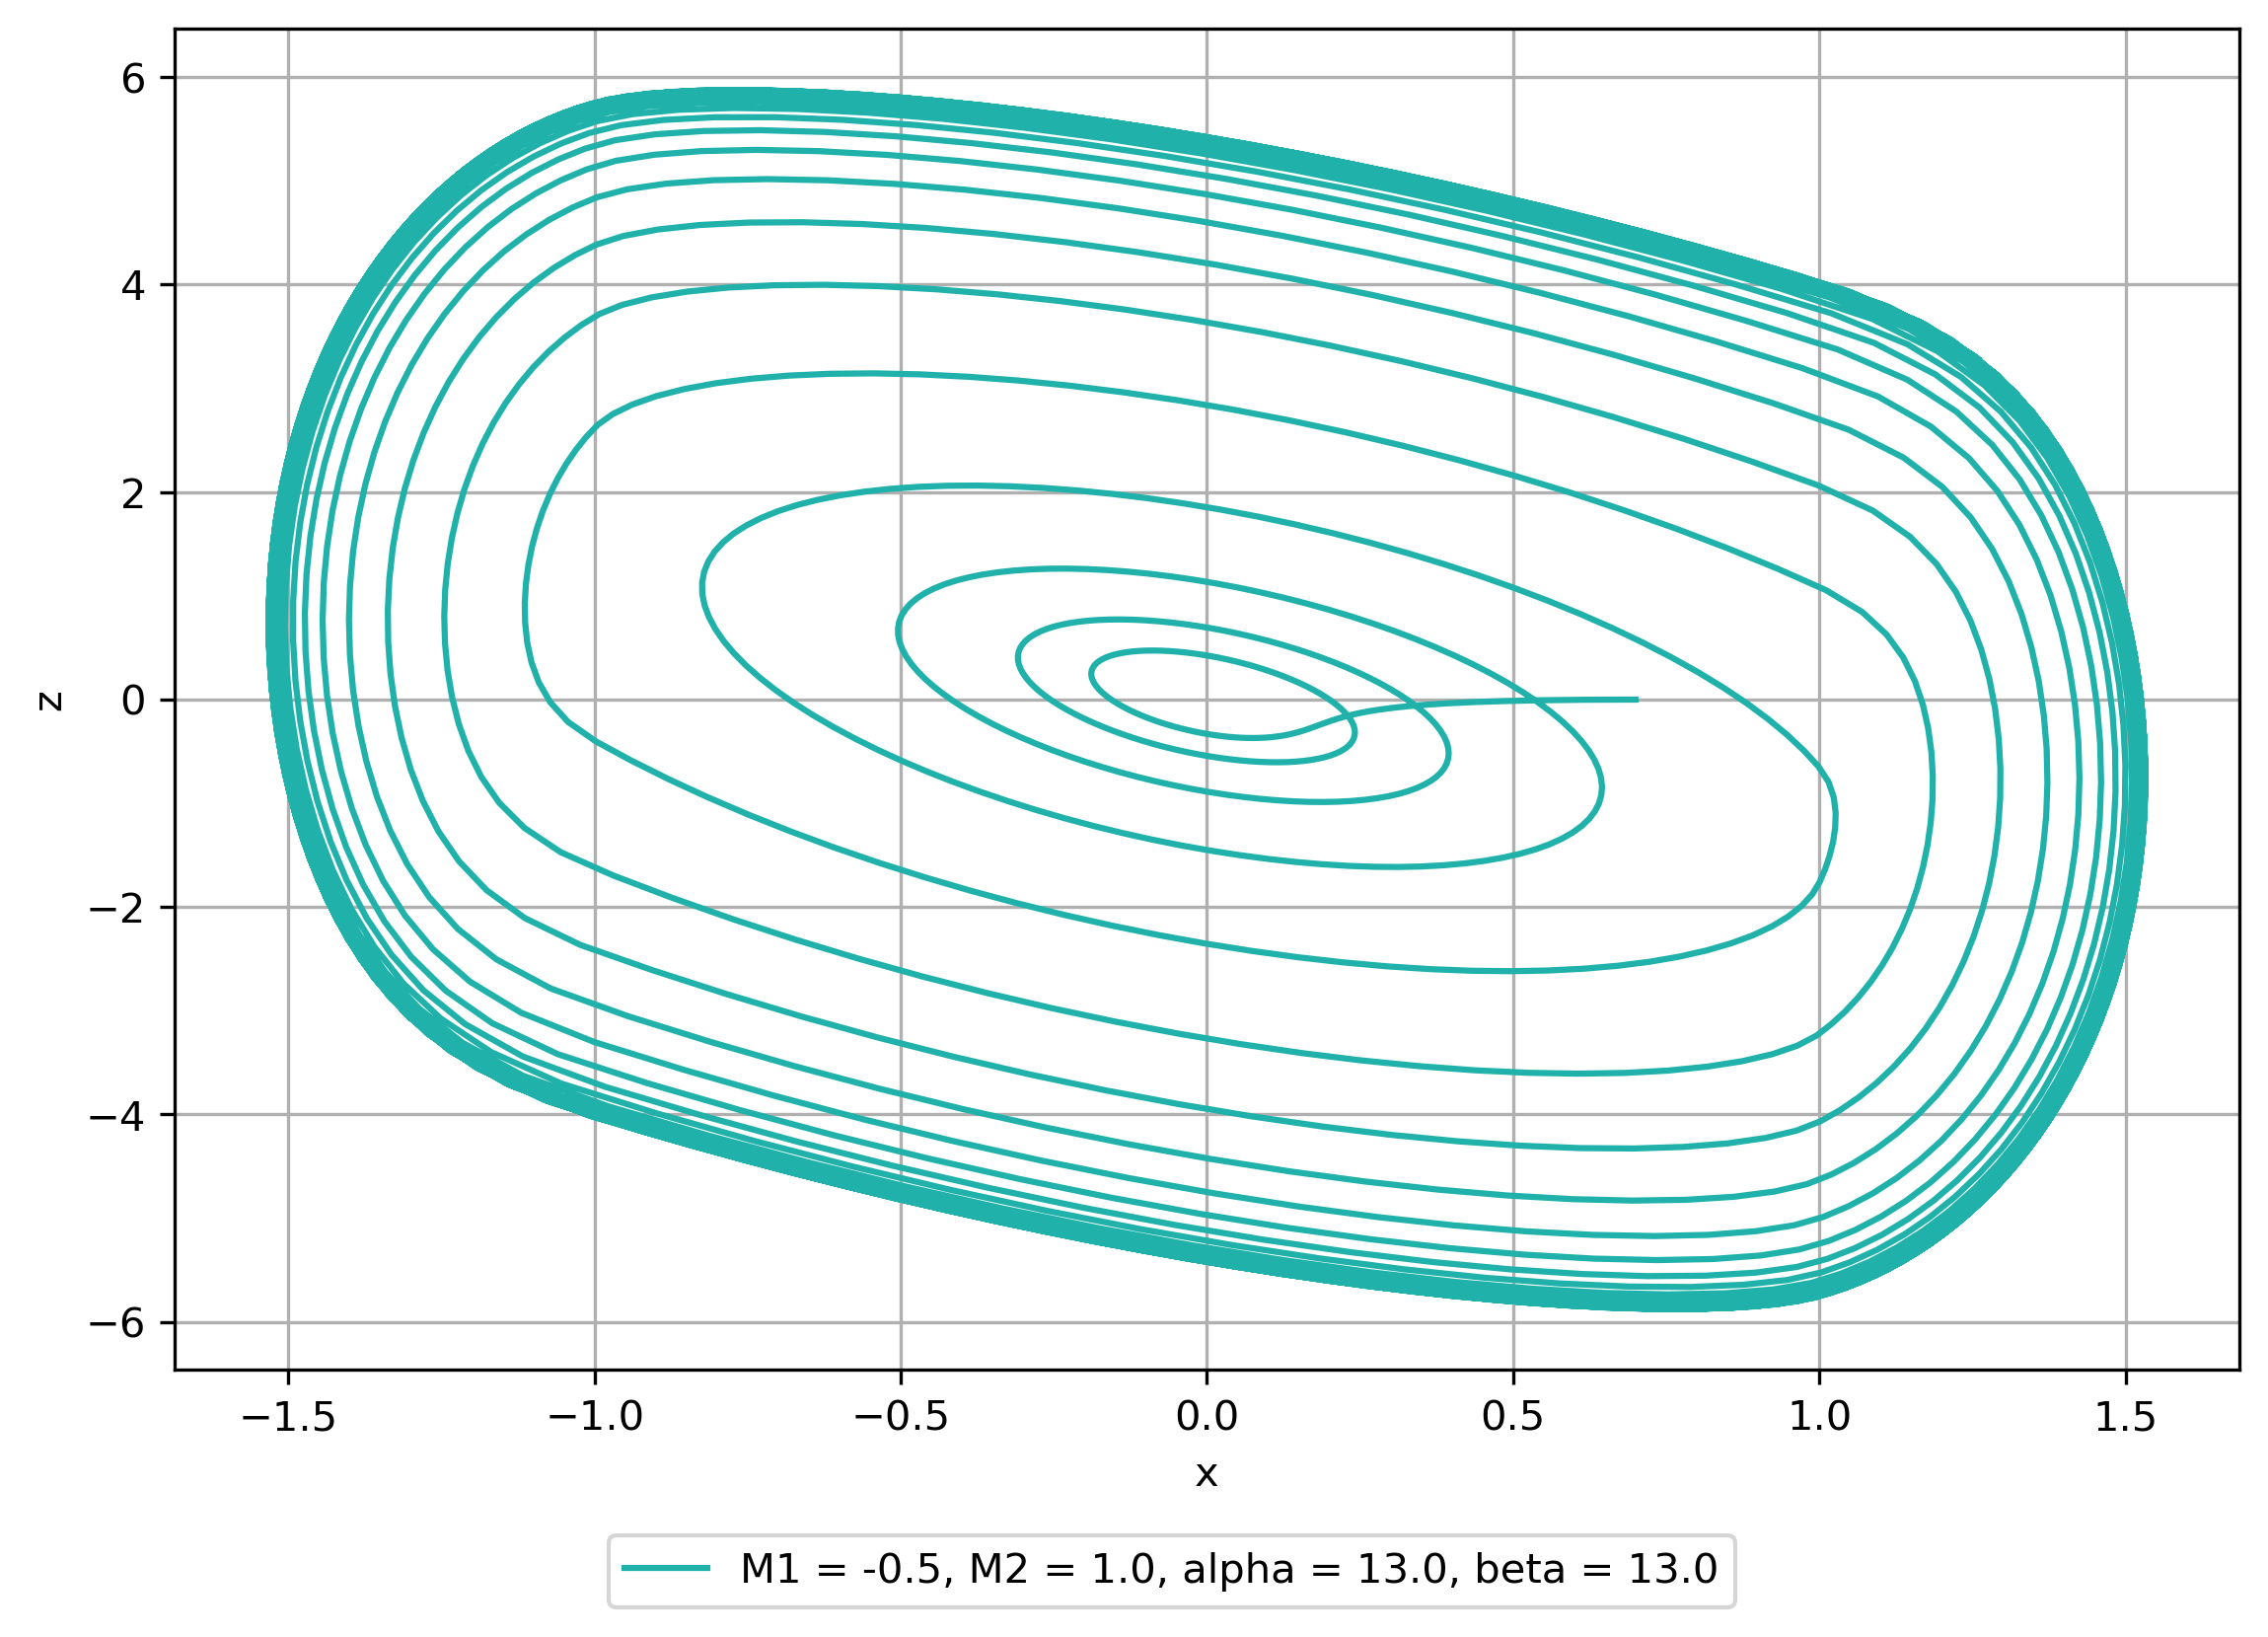
\includegraphics[width=0.3\textwidth]{attachments/fig.1.2.x-z.png}
				}
				\subfloat[y-z plain]{
				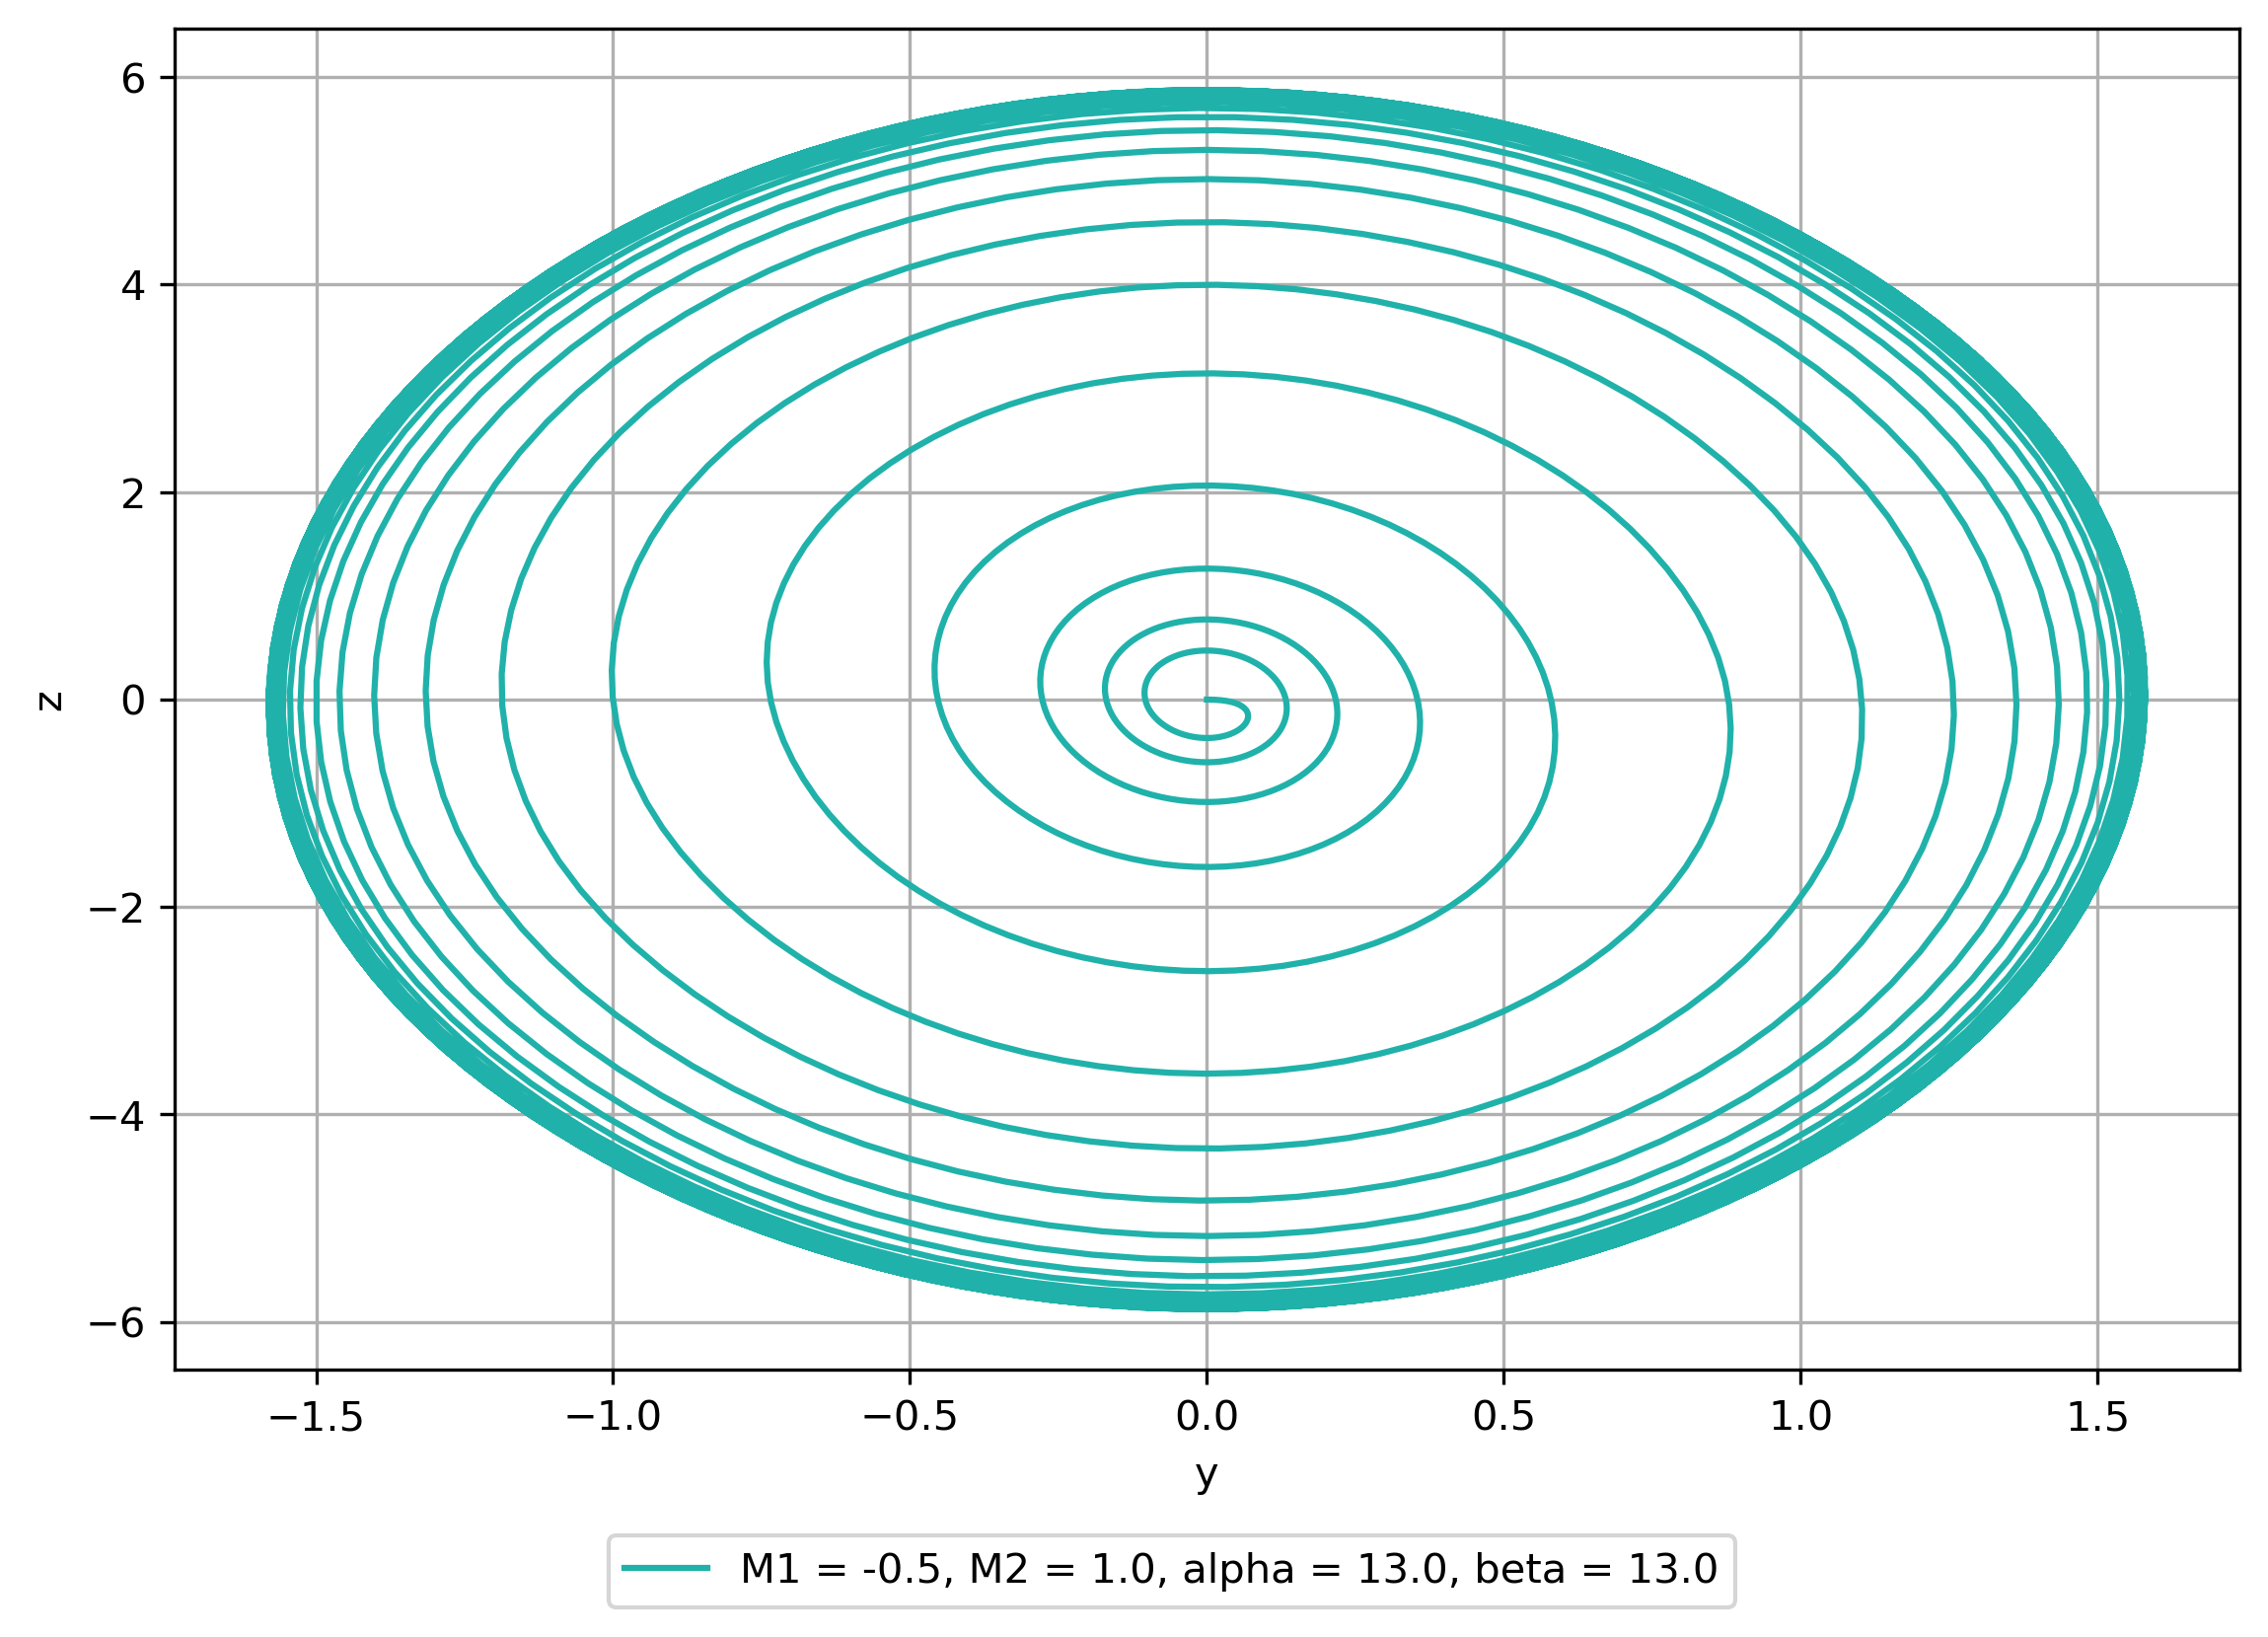
\includegraphics[width=0.3\textwidth]{attachments/fig.1.2.y-z.png}
				}
				\caption{\textbf{Numerical calculation of Chua's circuit, limit ring}}
				\label{fig.1.2}
			\end{figure*}
			
			\begin{figure*}[htbp]
				\centering
				\subfloat[Channel]{
				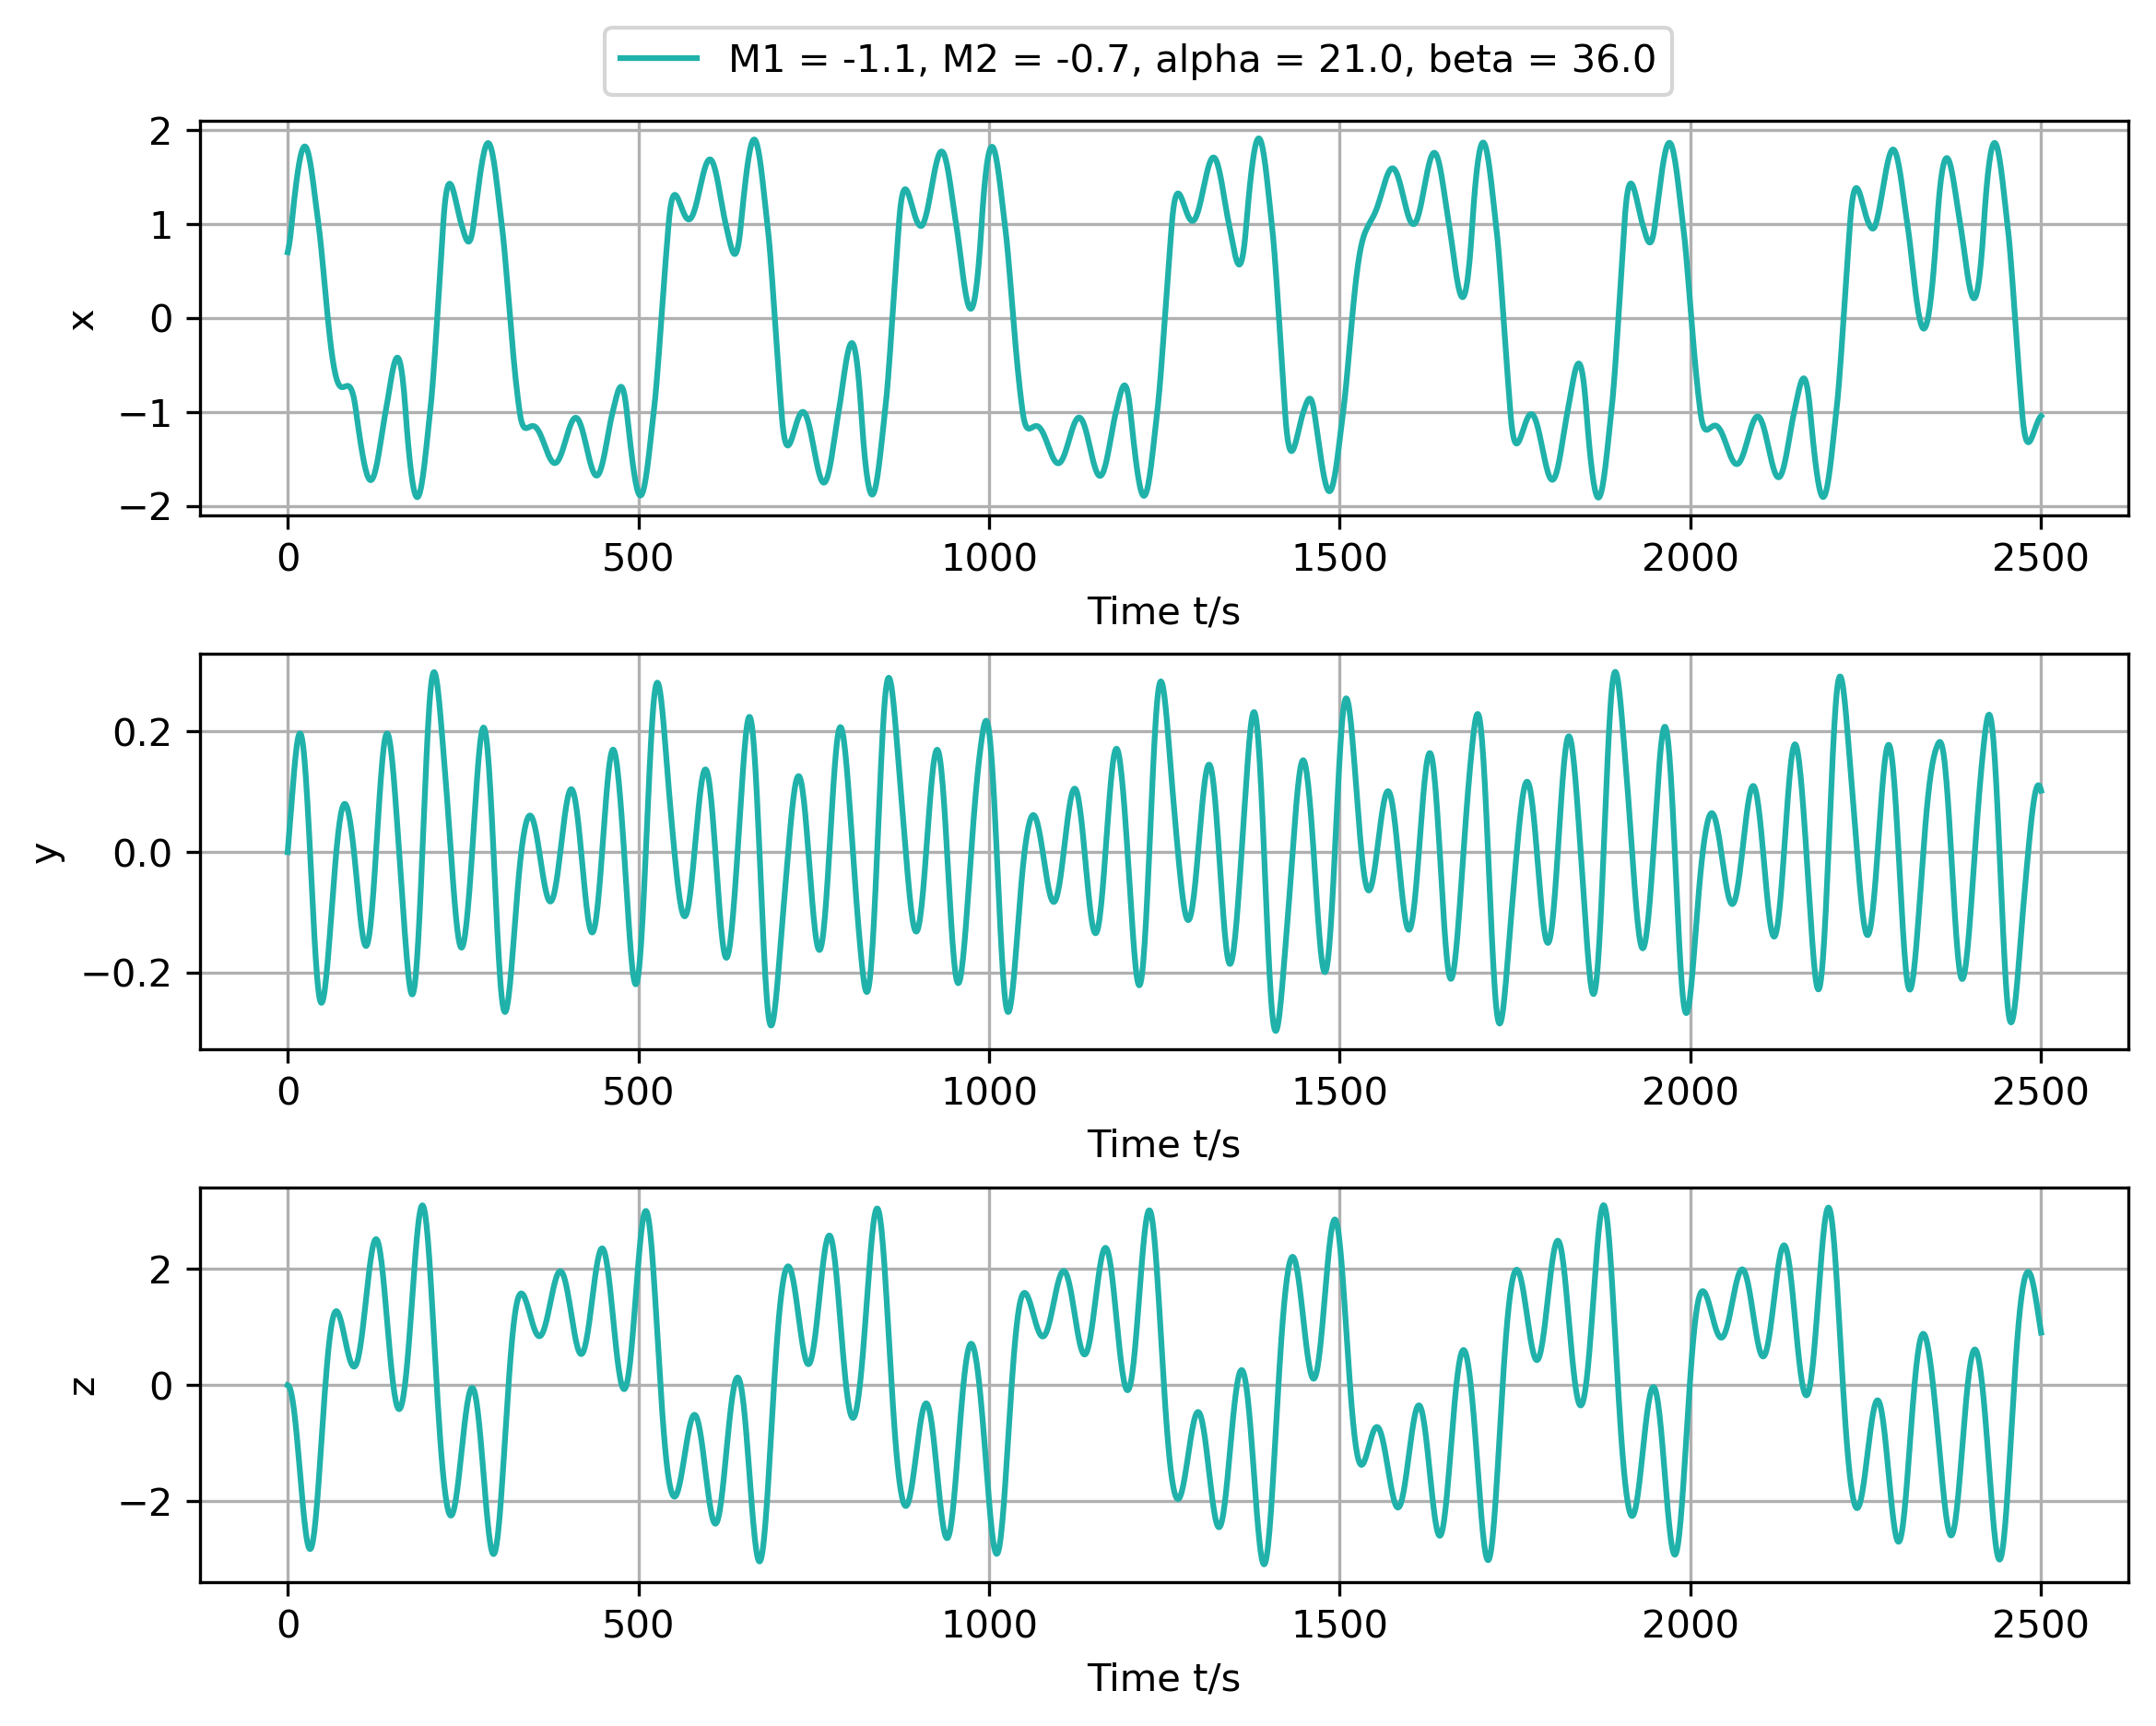
\includegraphics[width=0.3\textwidth]{attachments/fig.1.3.wave.png}
				}
				\subfloat[3d trace]{
				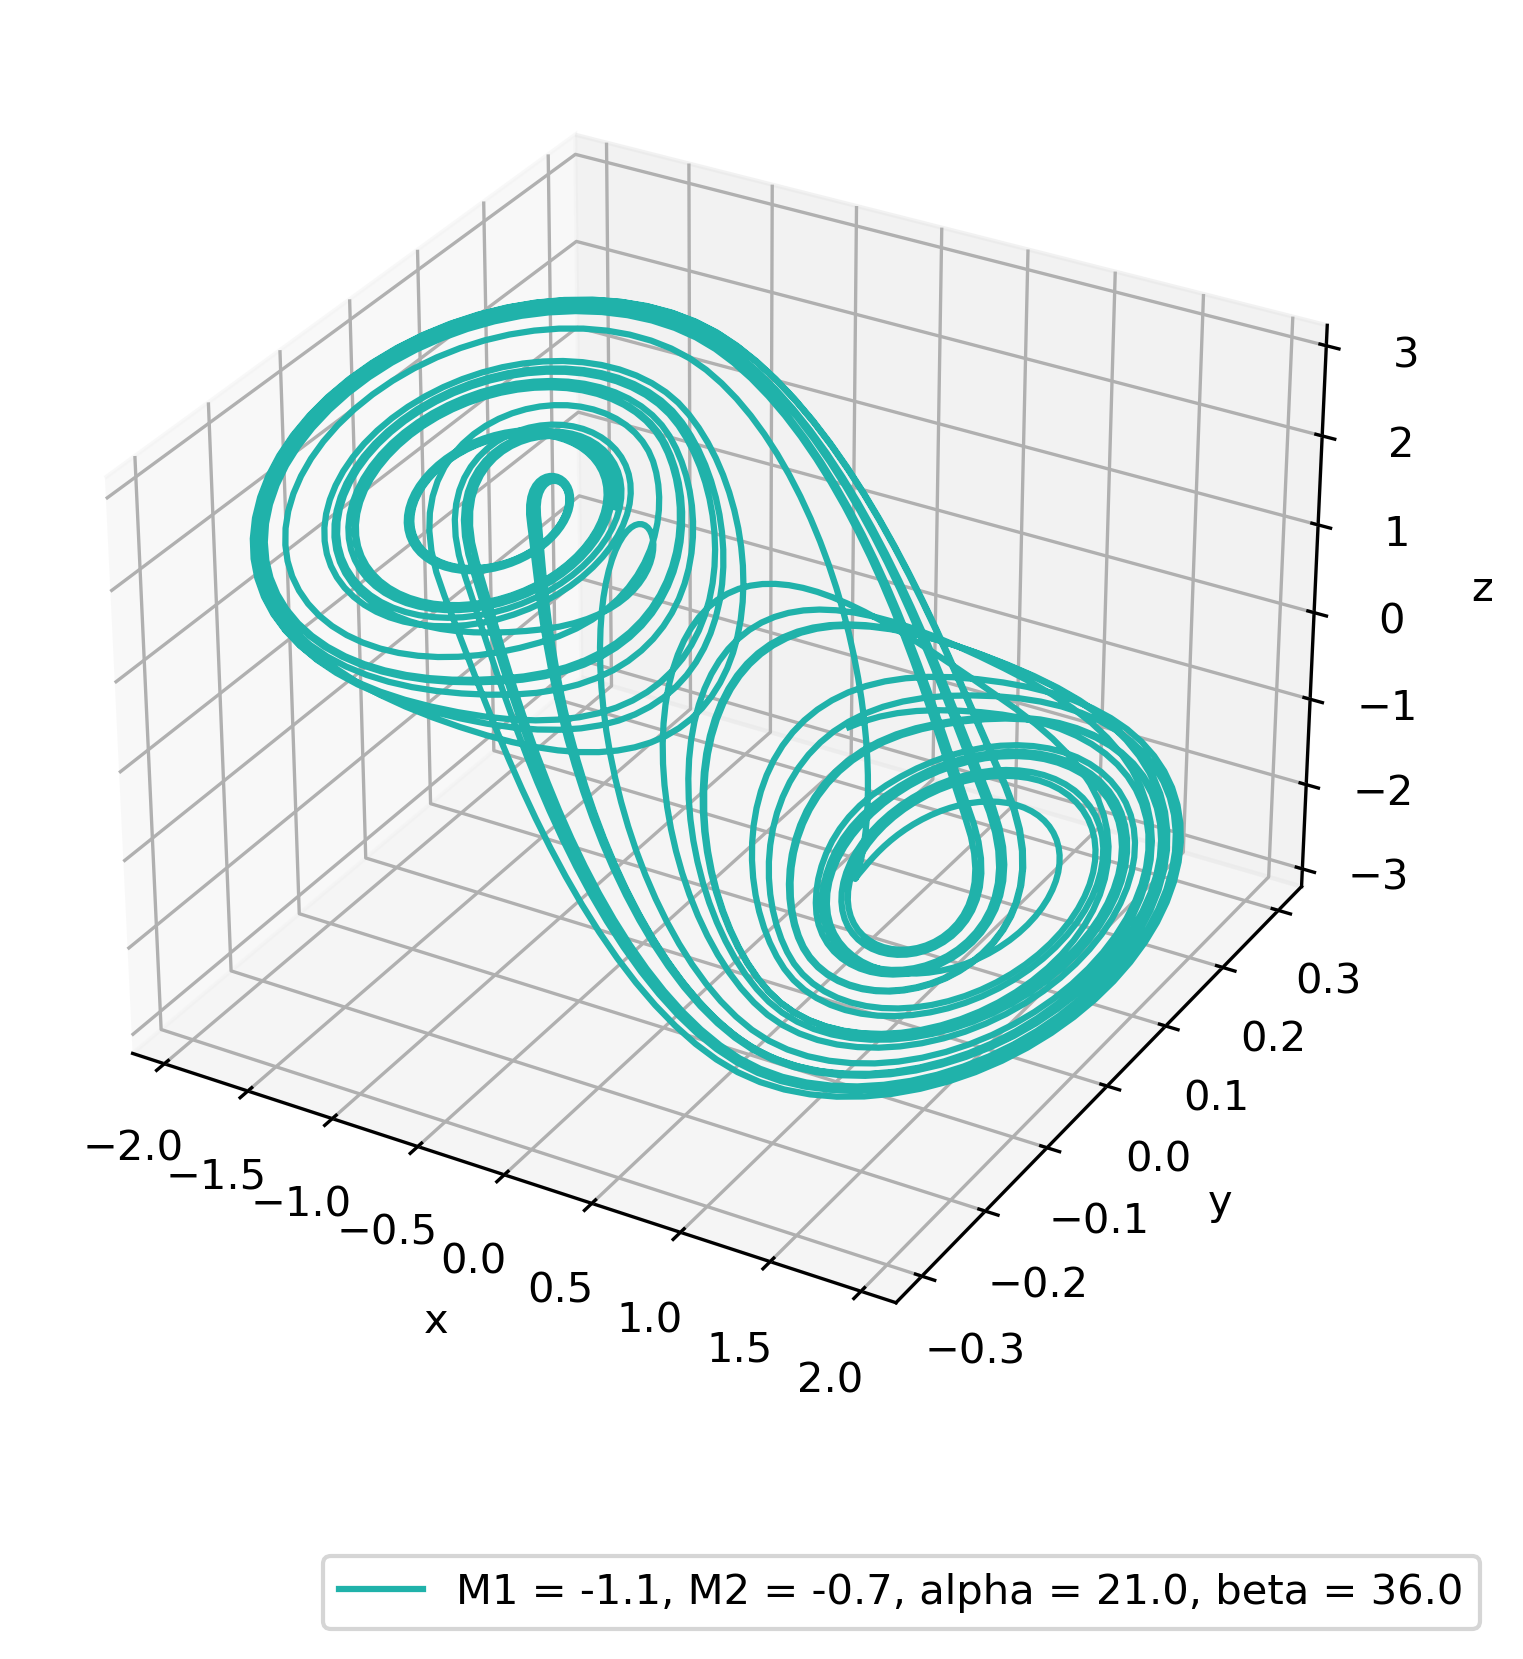
\includegraphics[width=0.3\textwidth]{attachments/fig.1.3.3d.png}
				}

				\subfloat[x-y plain]{
				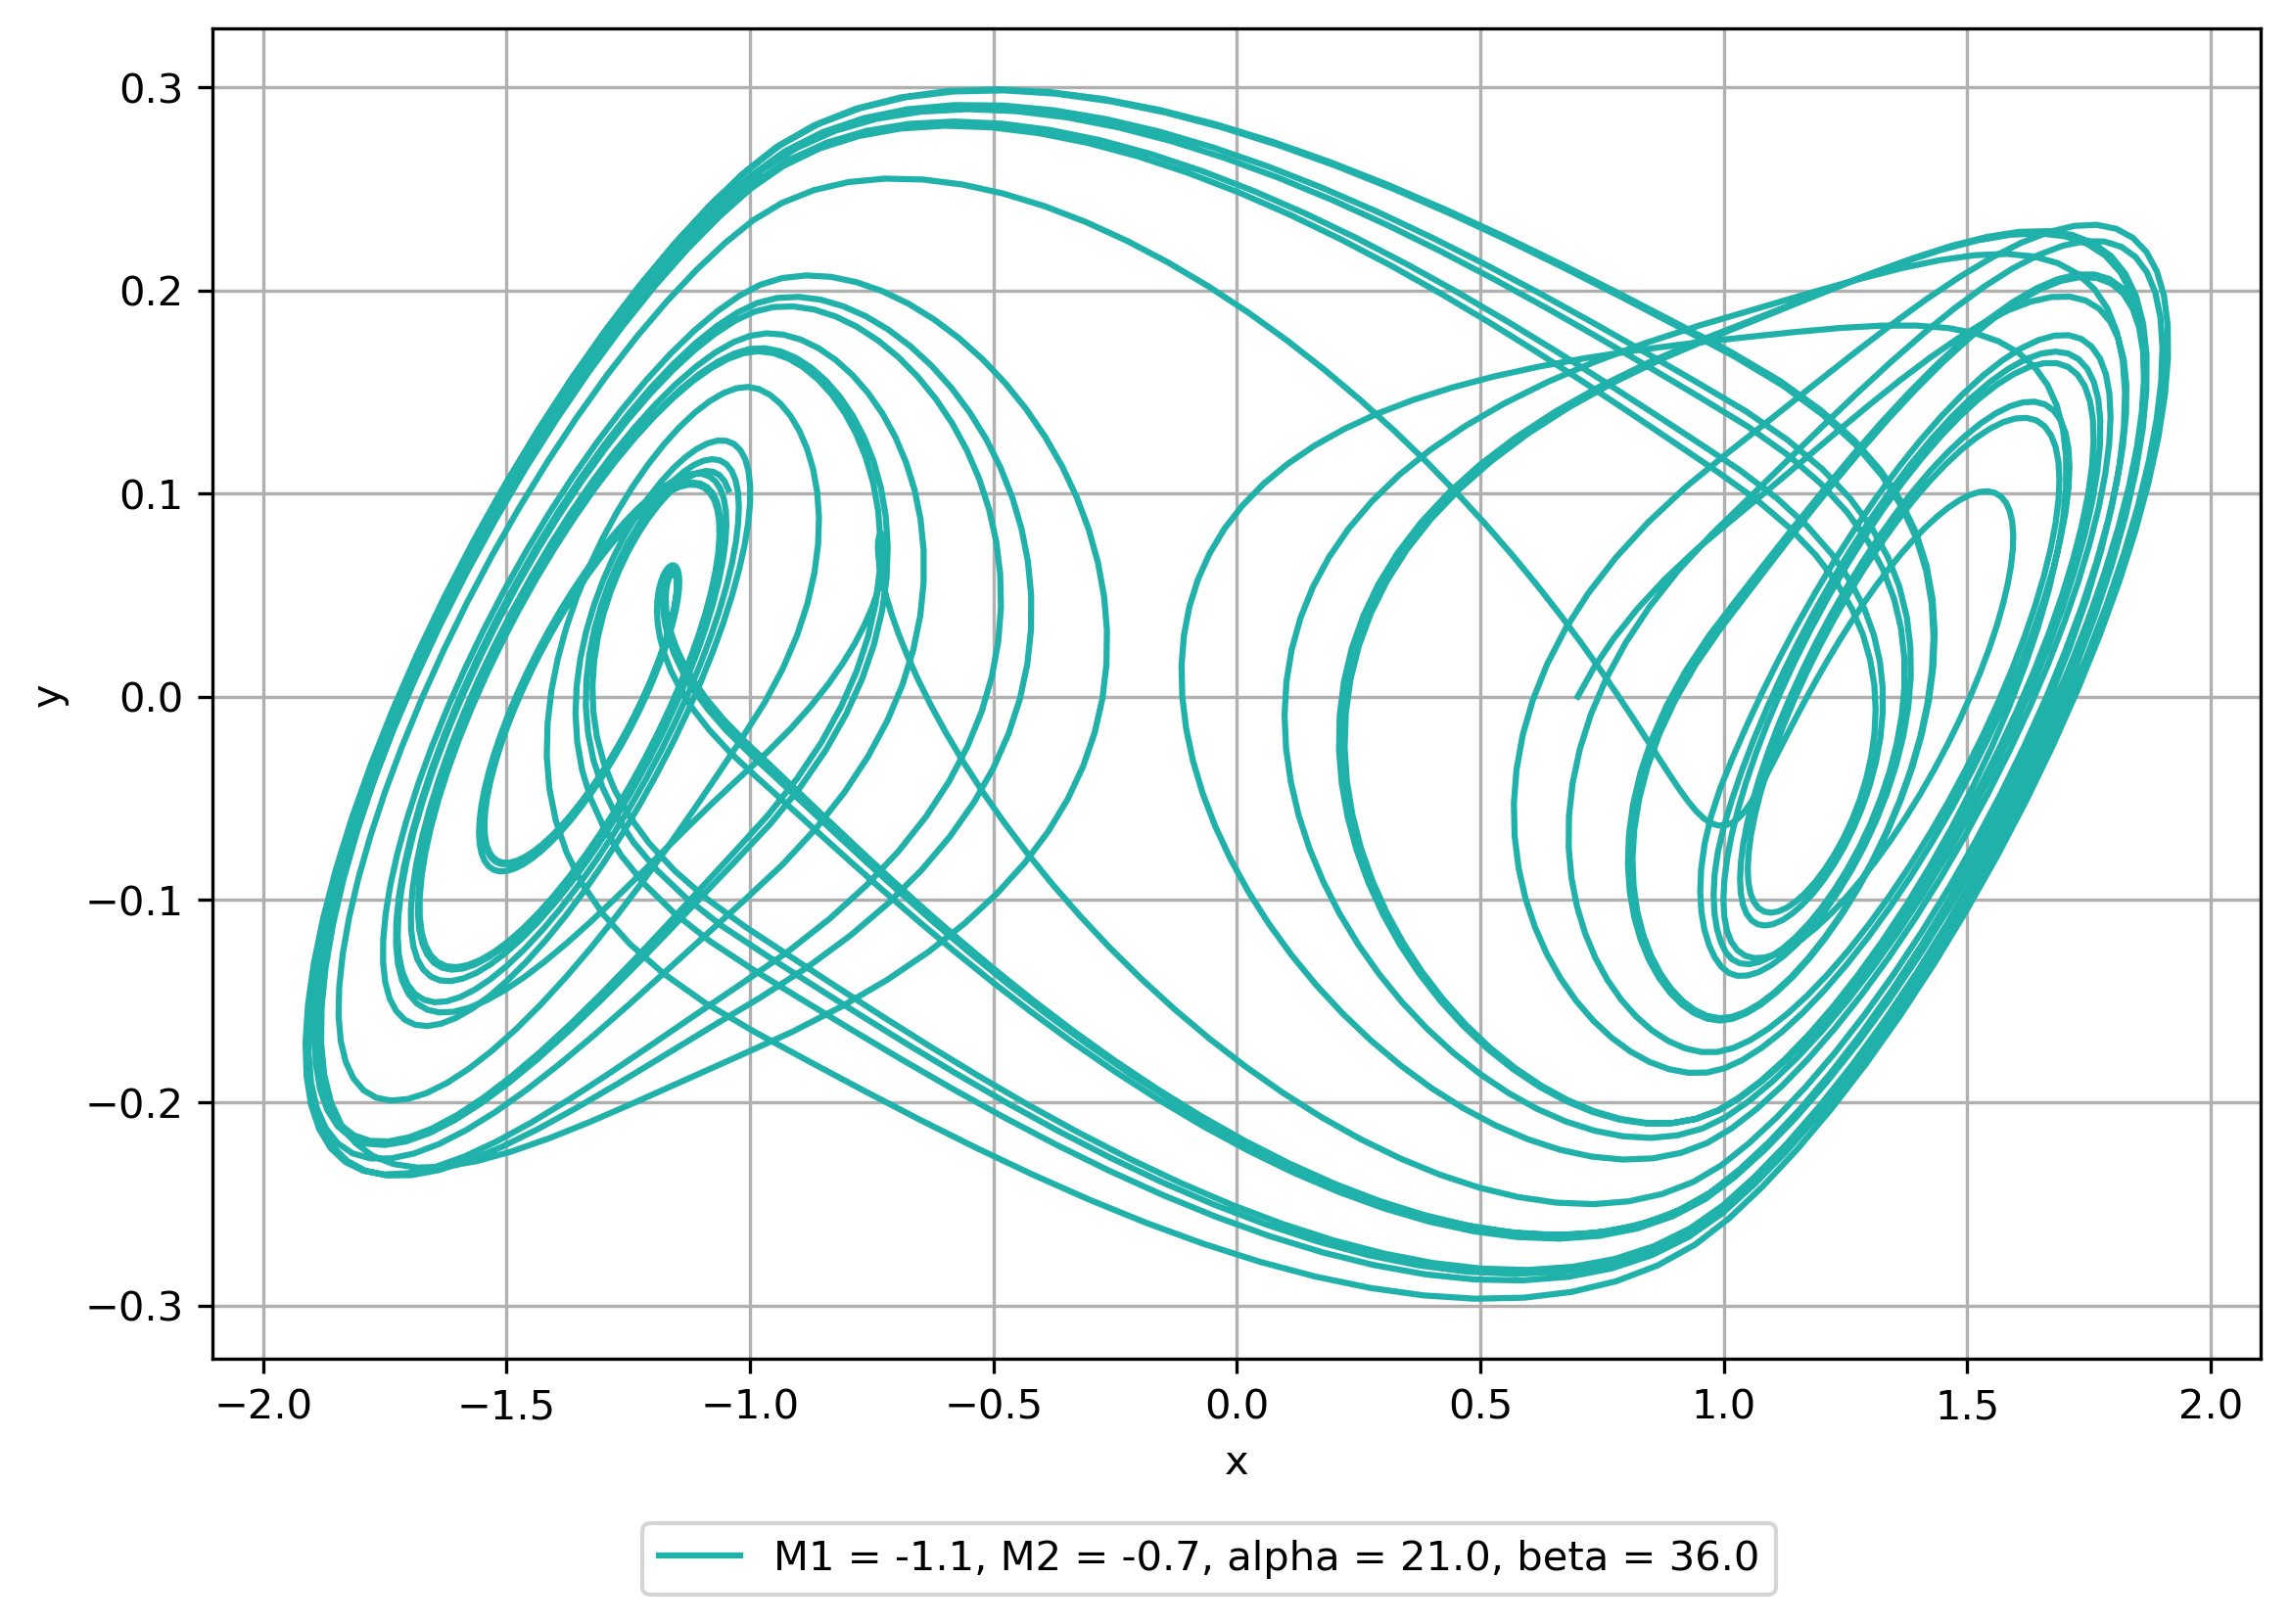
\includegraphics[width=0.3\textwidth]{attachments/fig.1.3.x-y.png}
				}
				\subfloat[x-z plain]{
				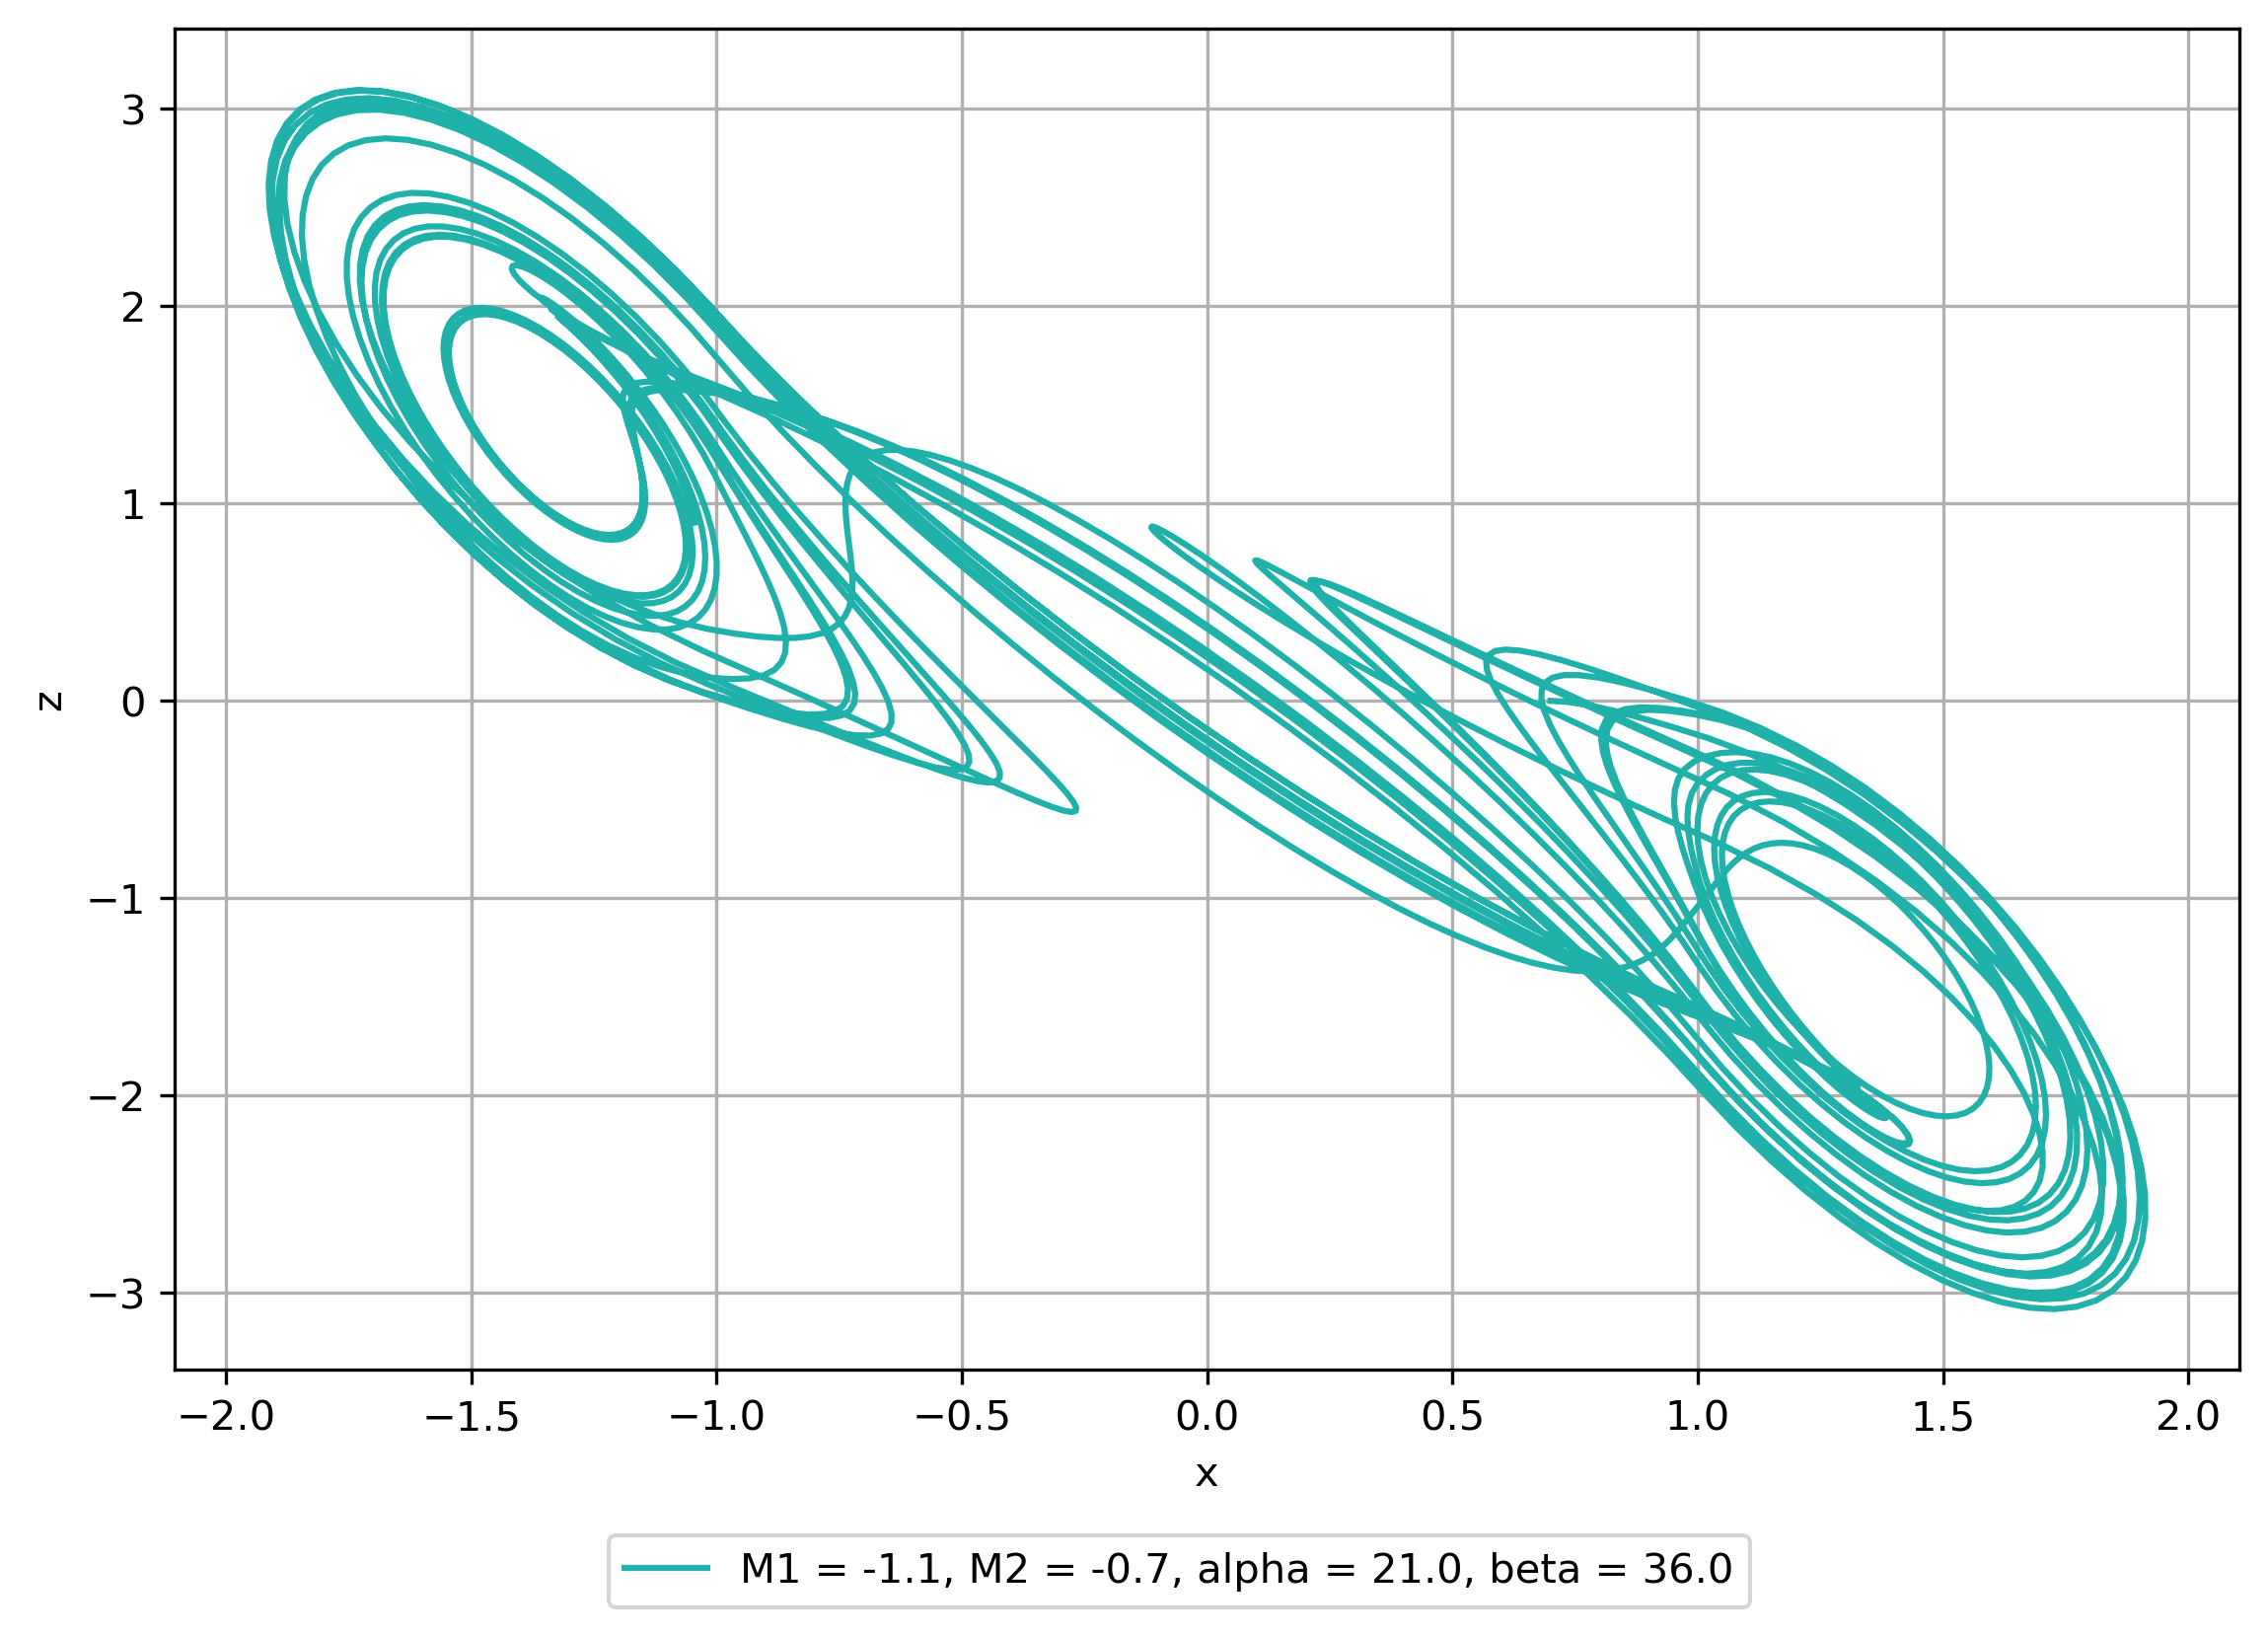
\includegraphics[width=0.3\textwidth]{attachments/fig.1.3.x-z.png}
				}
				\subfloat[y-z plain]{
				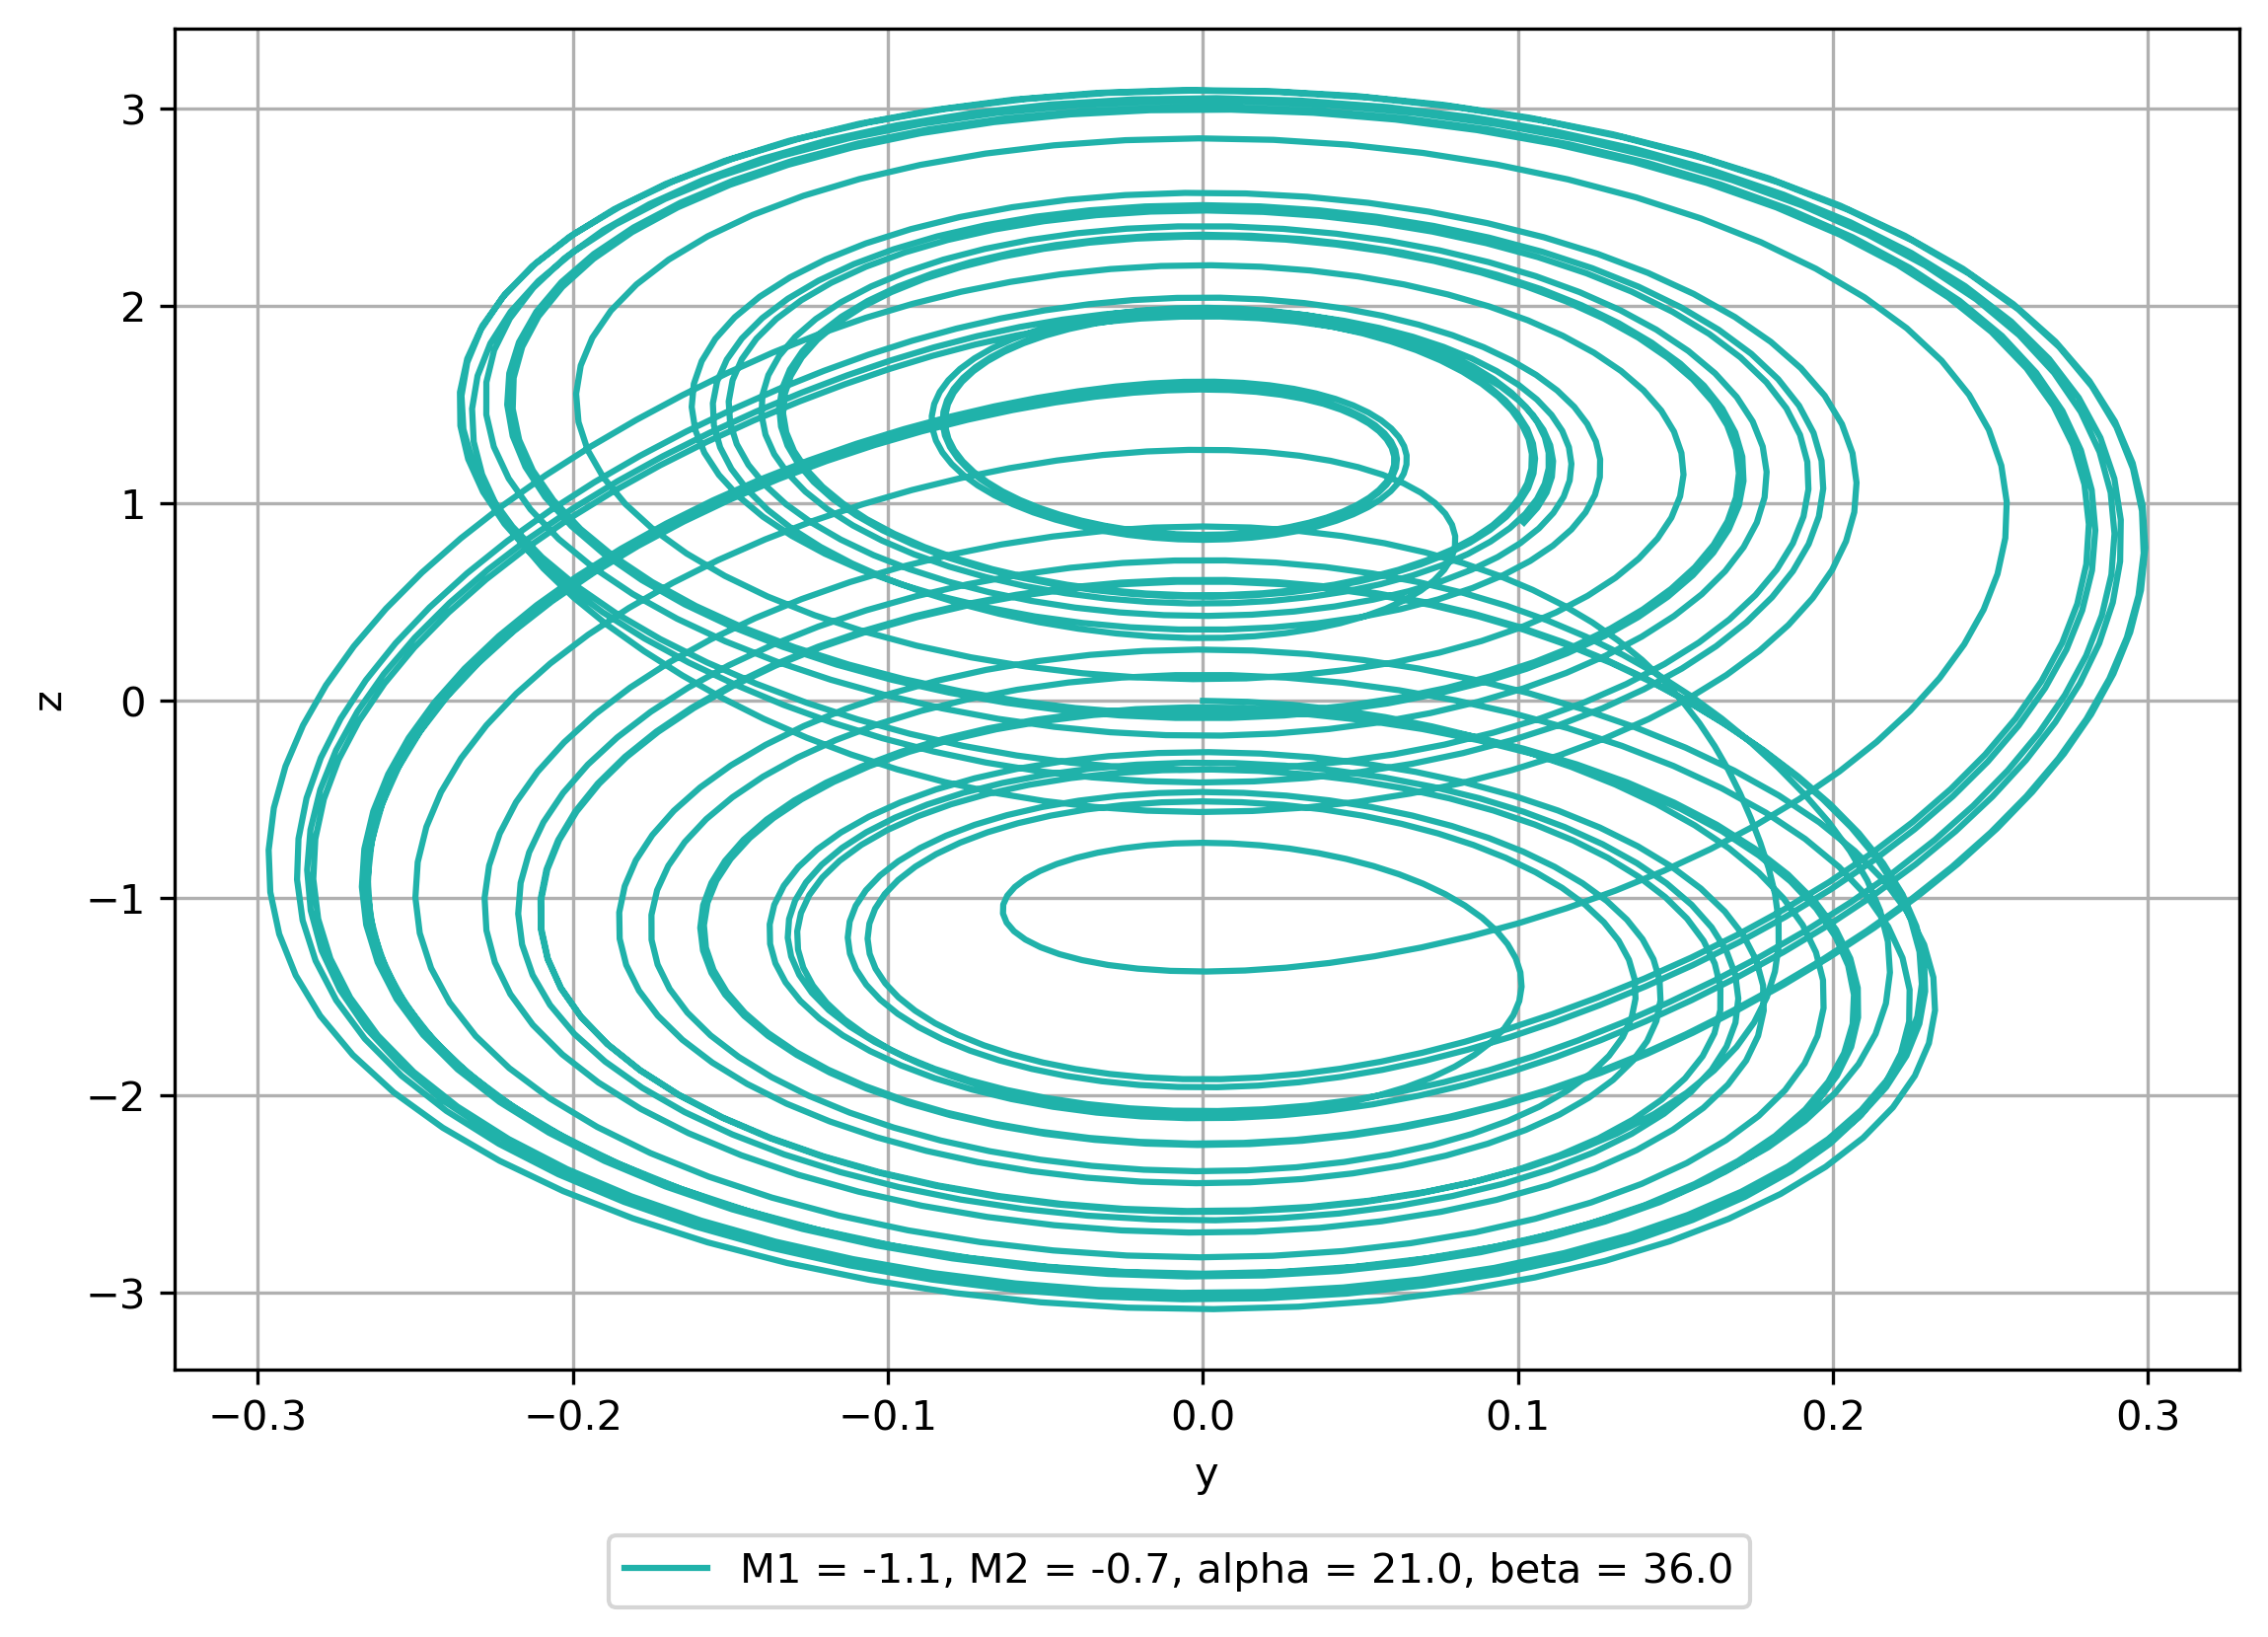
\includegraphics[width=0.3\textwidth]{attachments/fig.1.3.y-z.png}
				}
				\caption{\textbf{Numerical calculation of Chua's circuit, double attractors}}
				\label{fig.1.3}
			\end{figure*}

			\begin{figure*}[htbp]
				\centering
				\subfloat[Channel]{
				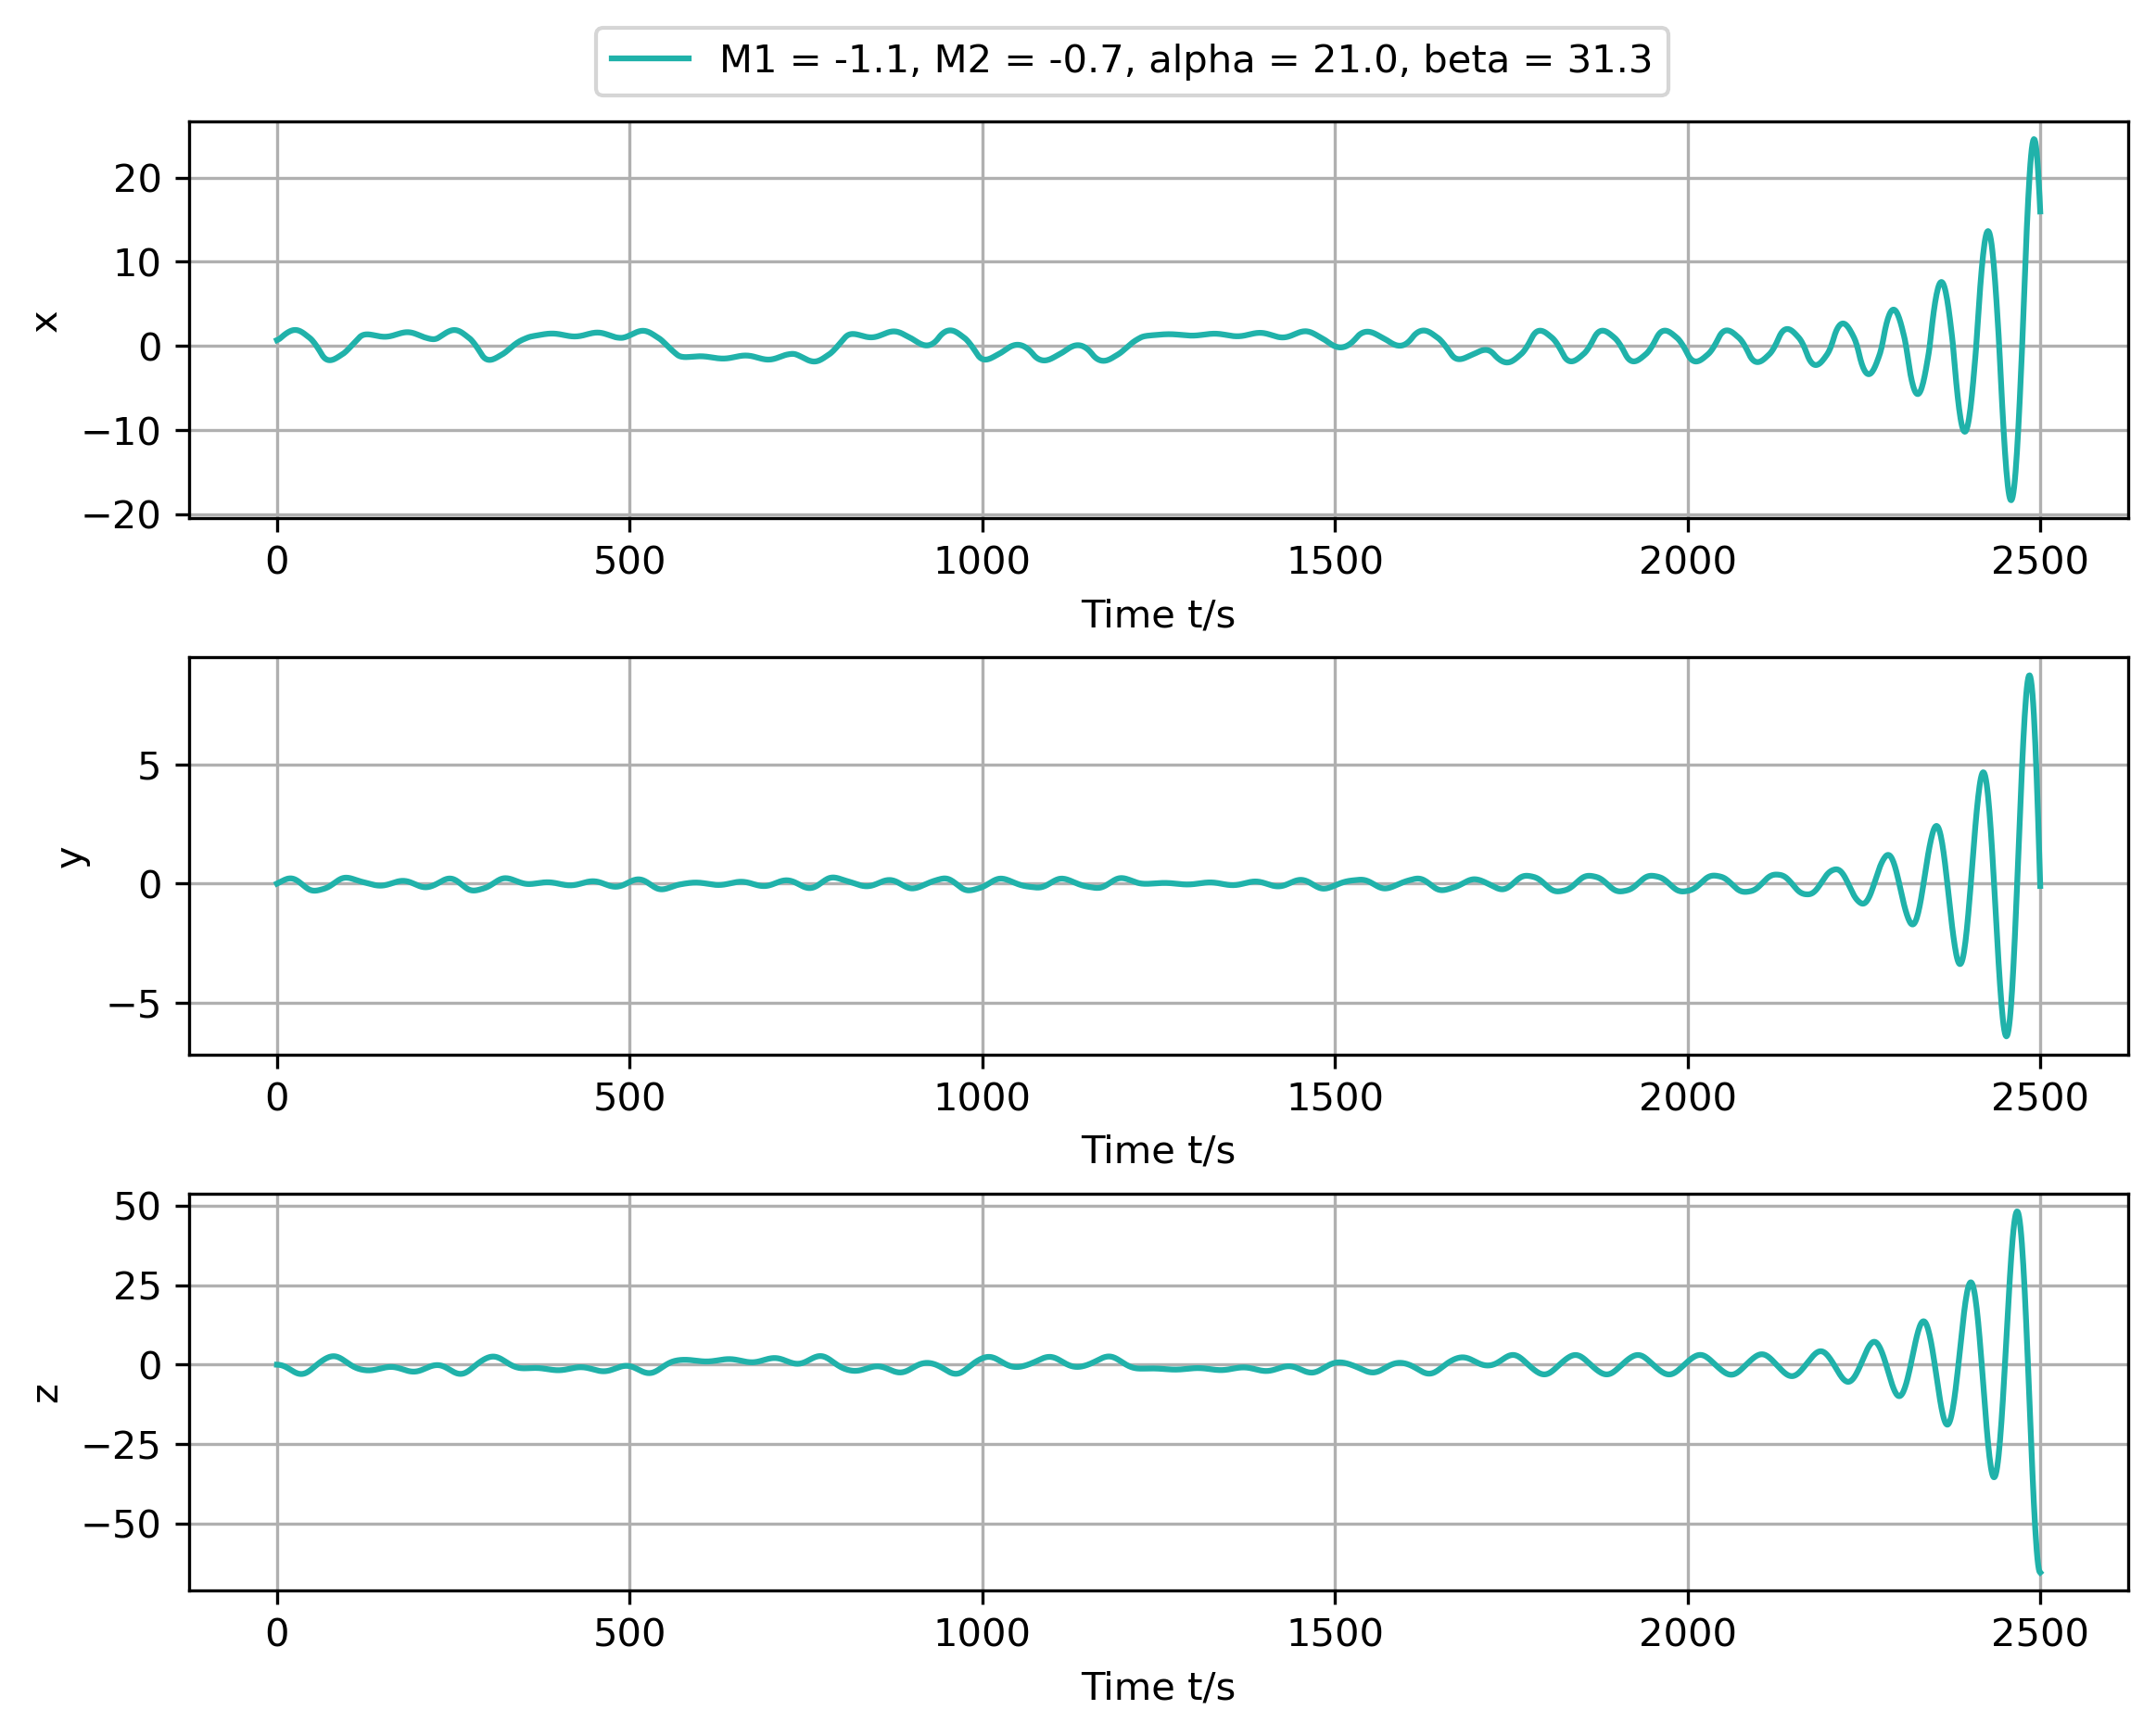
\includegraphics[width=0.3\textwidth]{attachments/fig.1.4.wave.png}
				}
				\subfloat[3d trace]{
				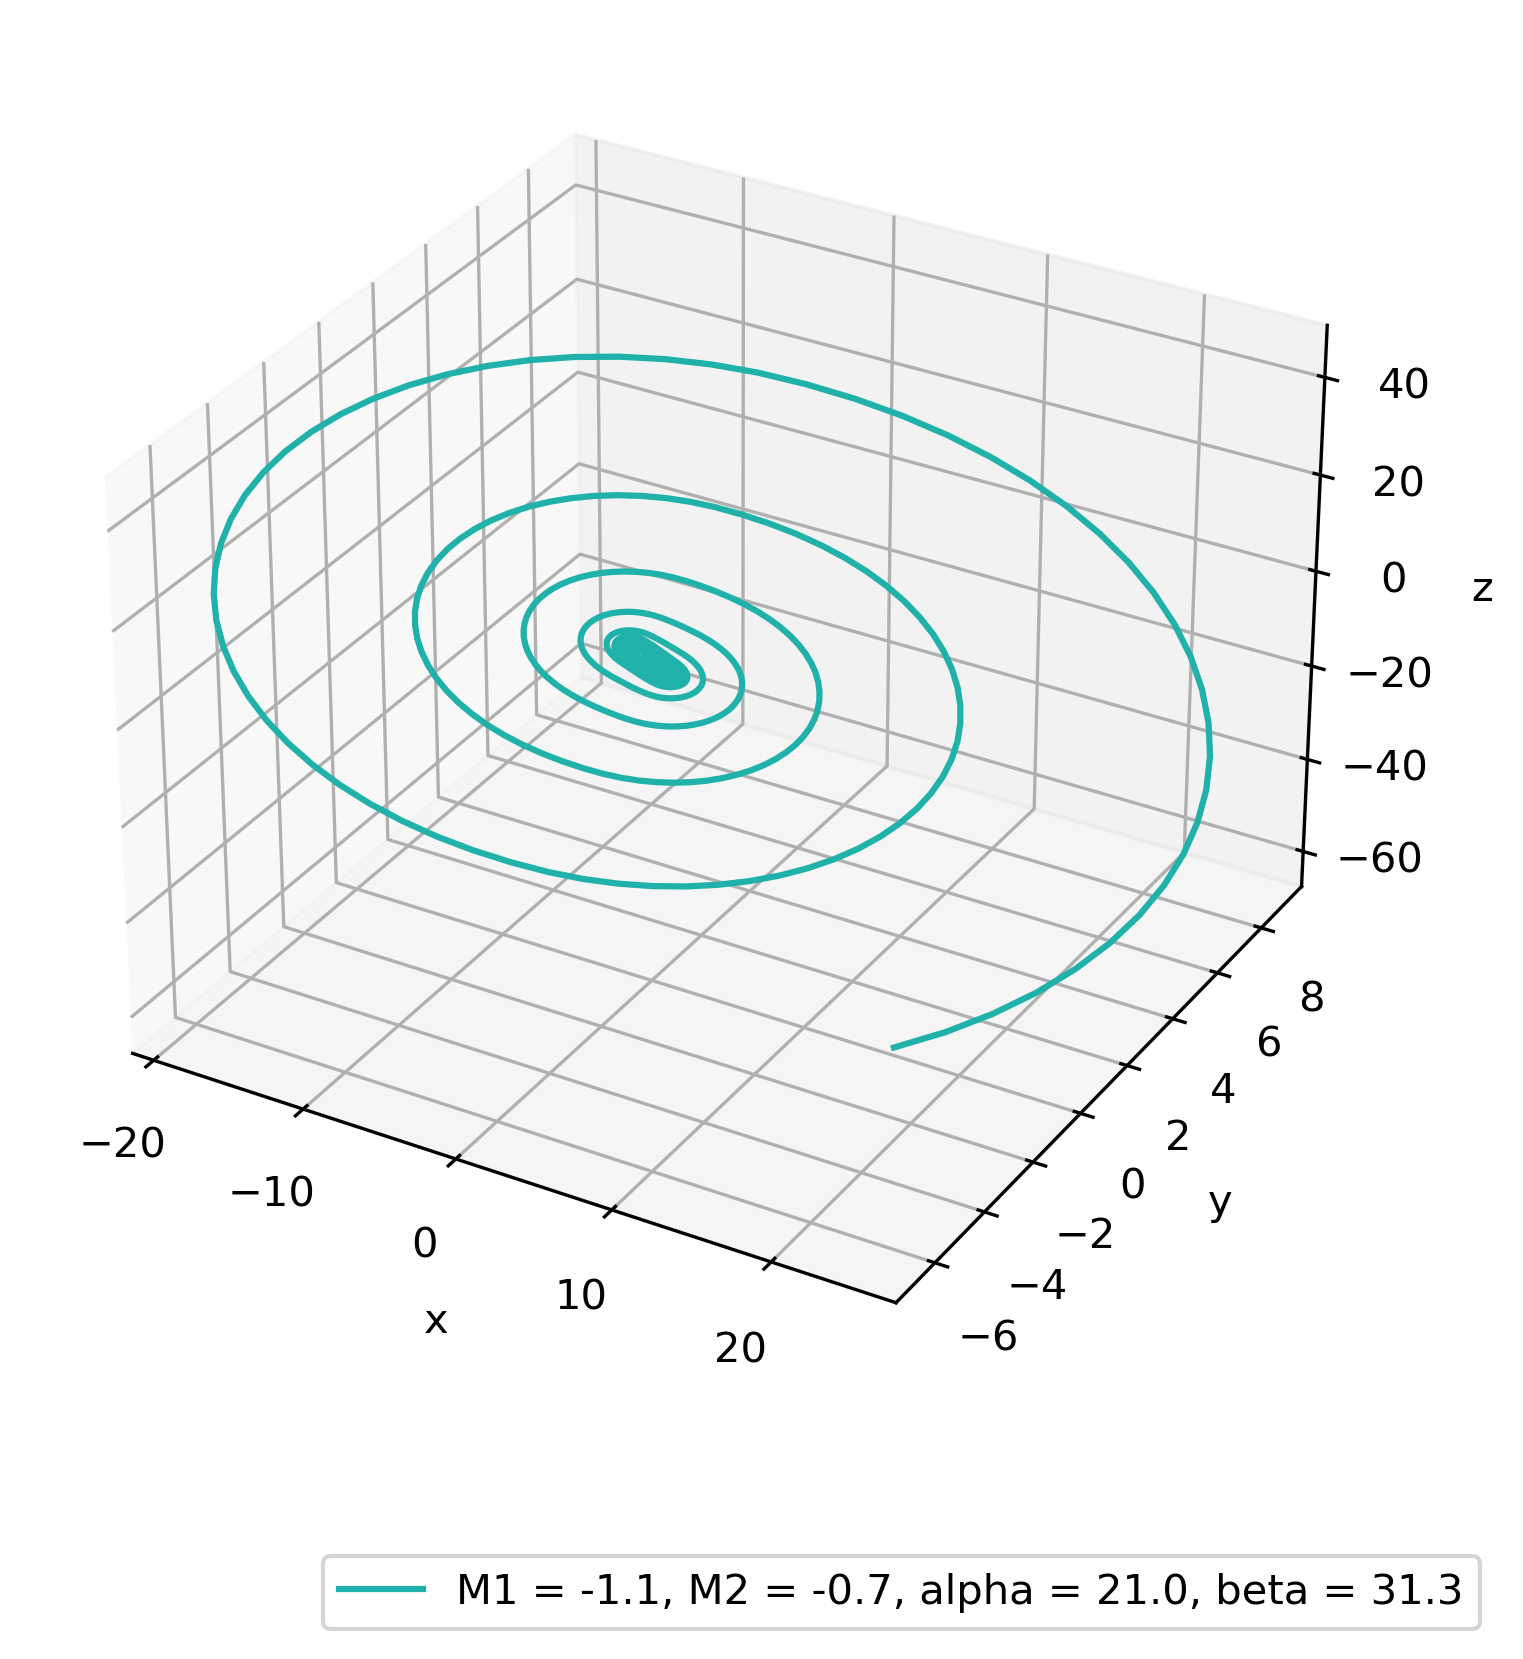
\includegraphics[width=0.3\textwidth]{attachments/fig.1.4.3d.png}
				}

				\subfloat[x-y plain]{
				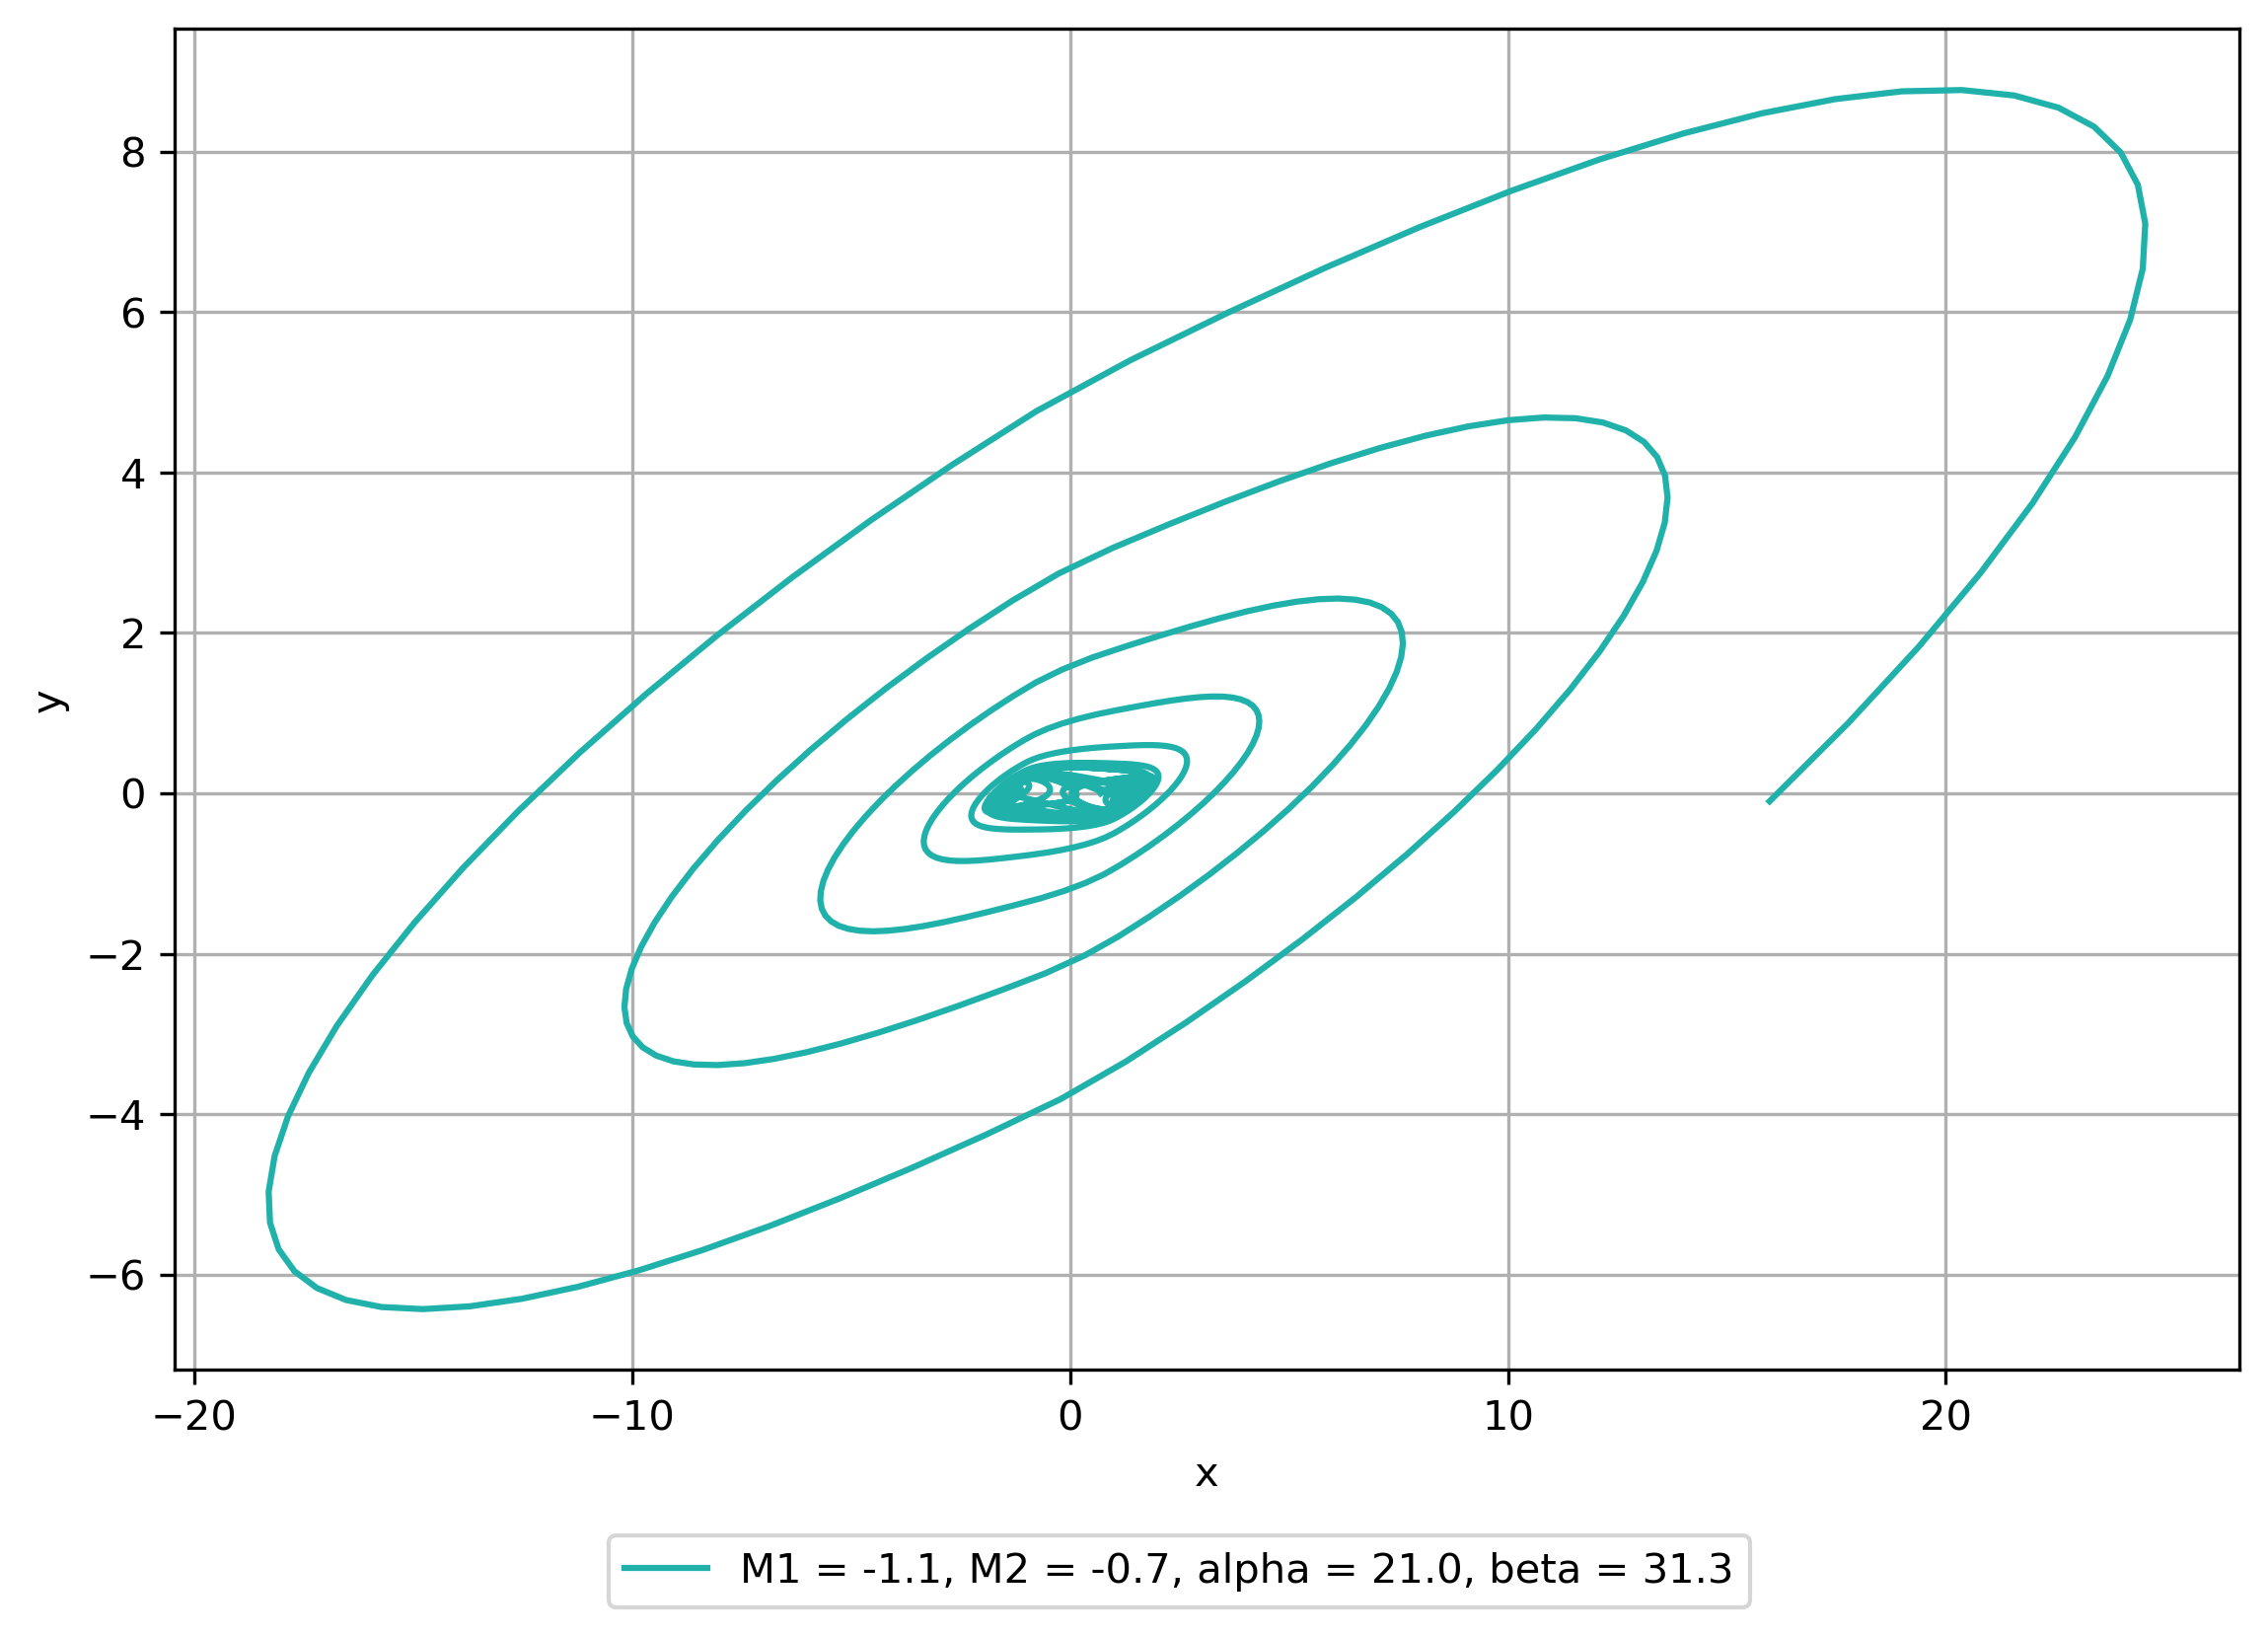
\includegraphics[width=0.3\textwidth]{attachments/fig.1.4.x-y.png}
				}
				\subfloat[x-z plain]{
				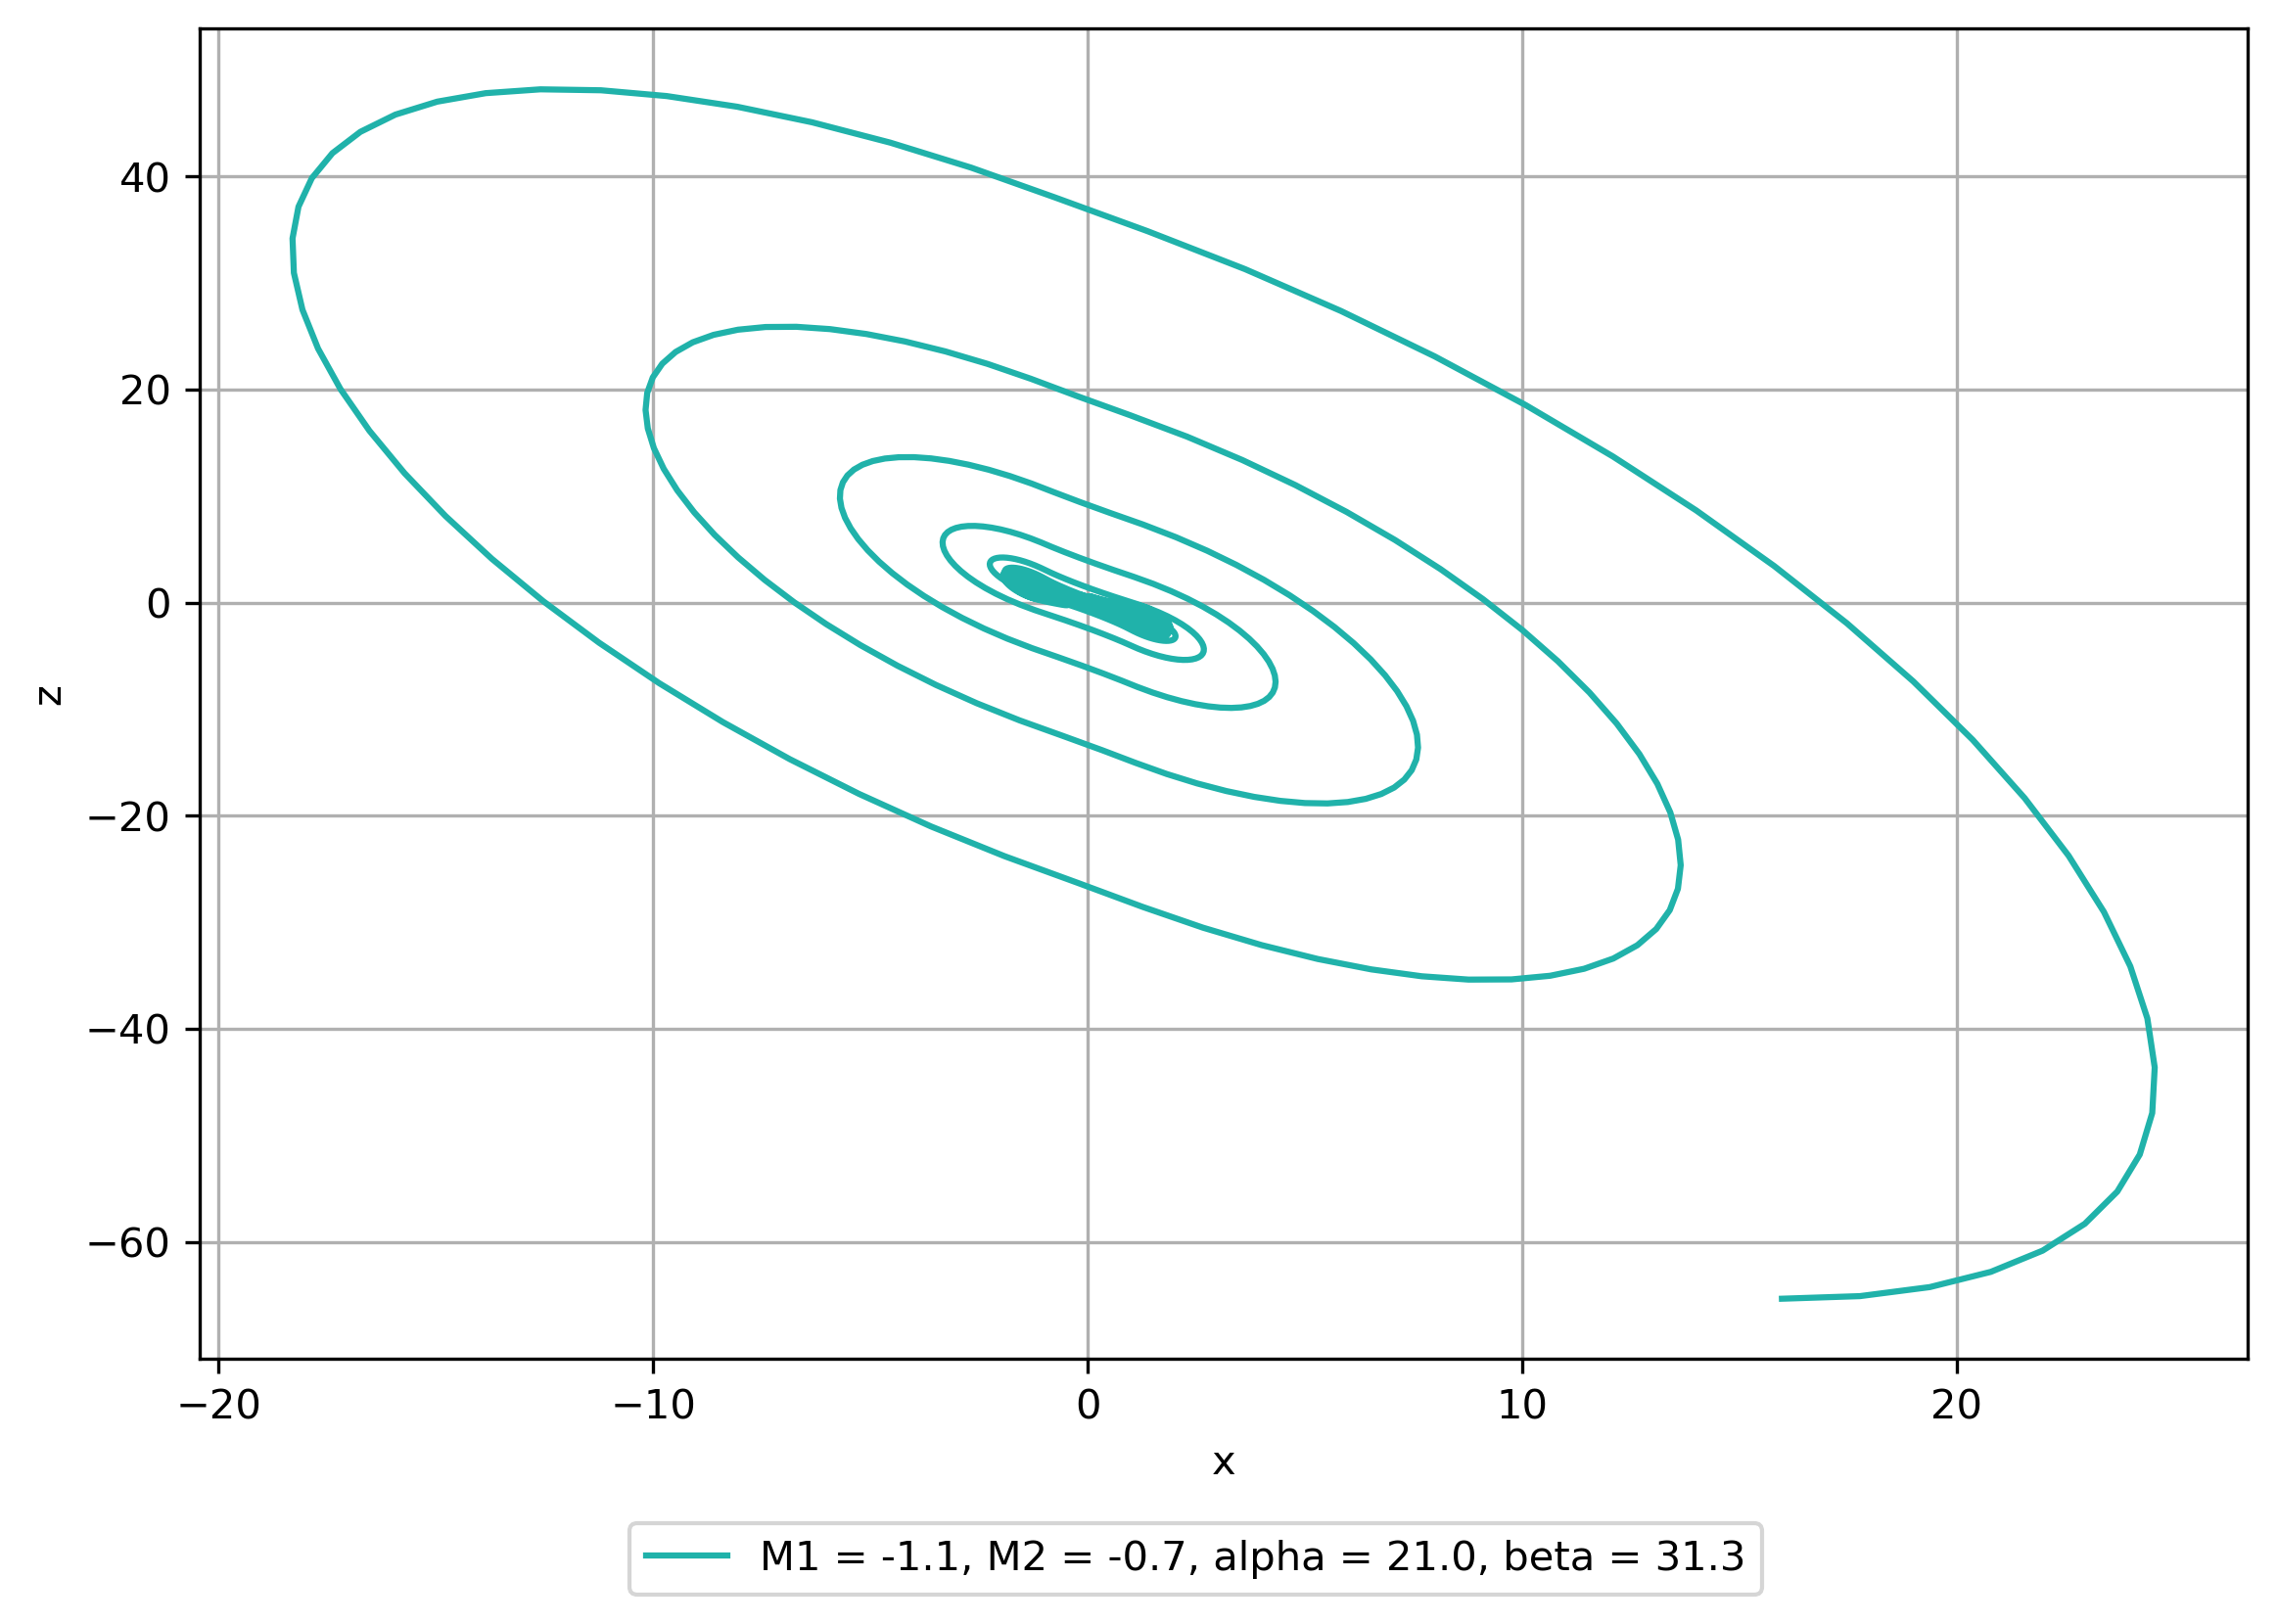
\includegraphics[width=0.3\textwidth]{attachments/fig.1.4.x-z.png}
				}
				\subfloat[y-z plain]{
				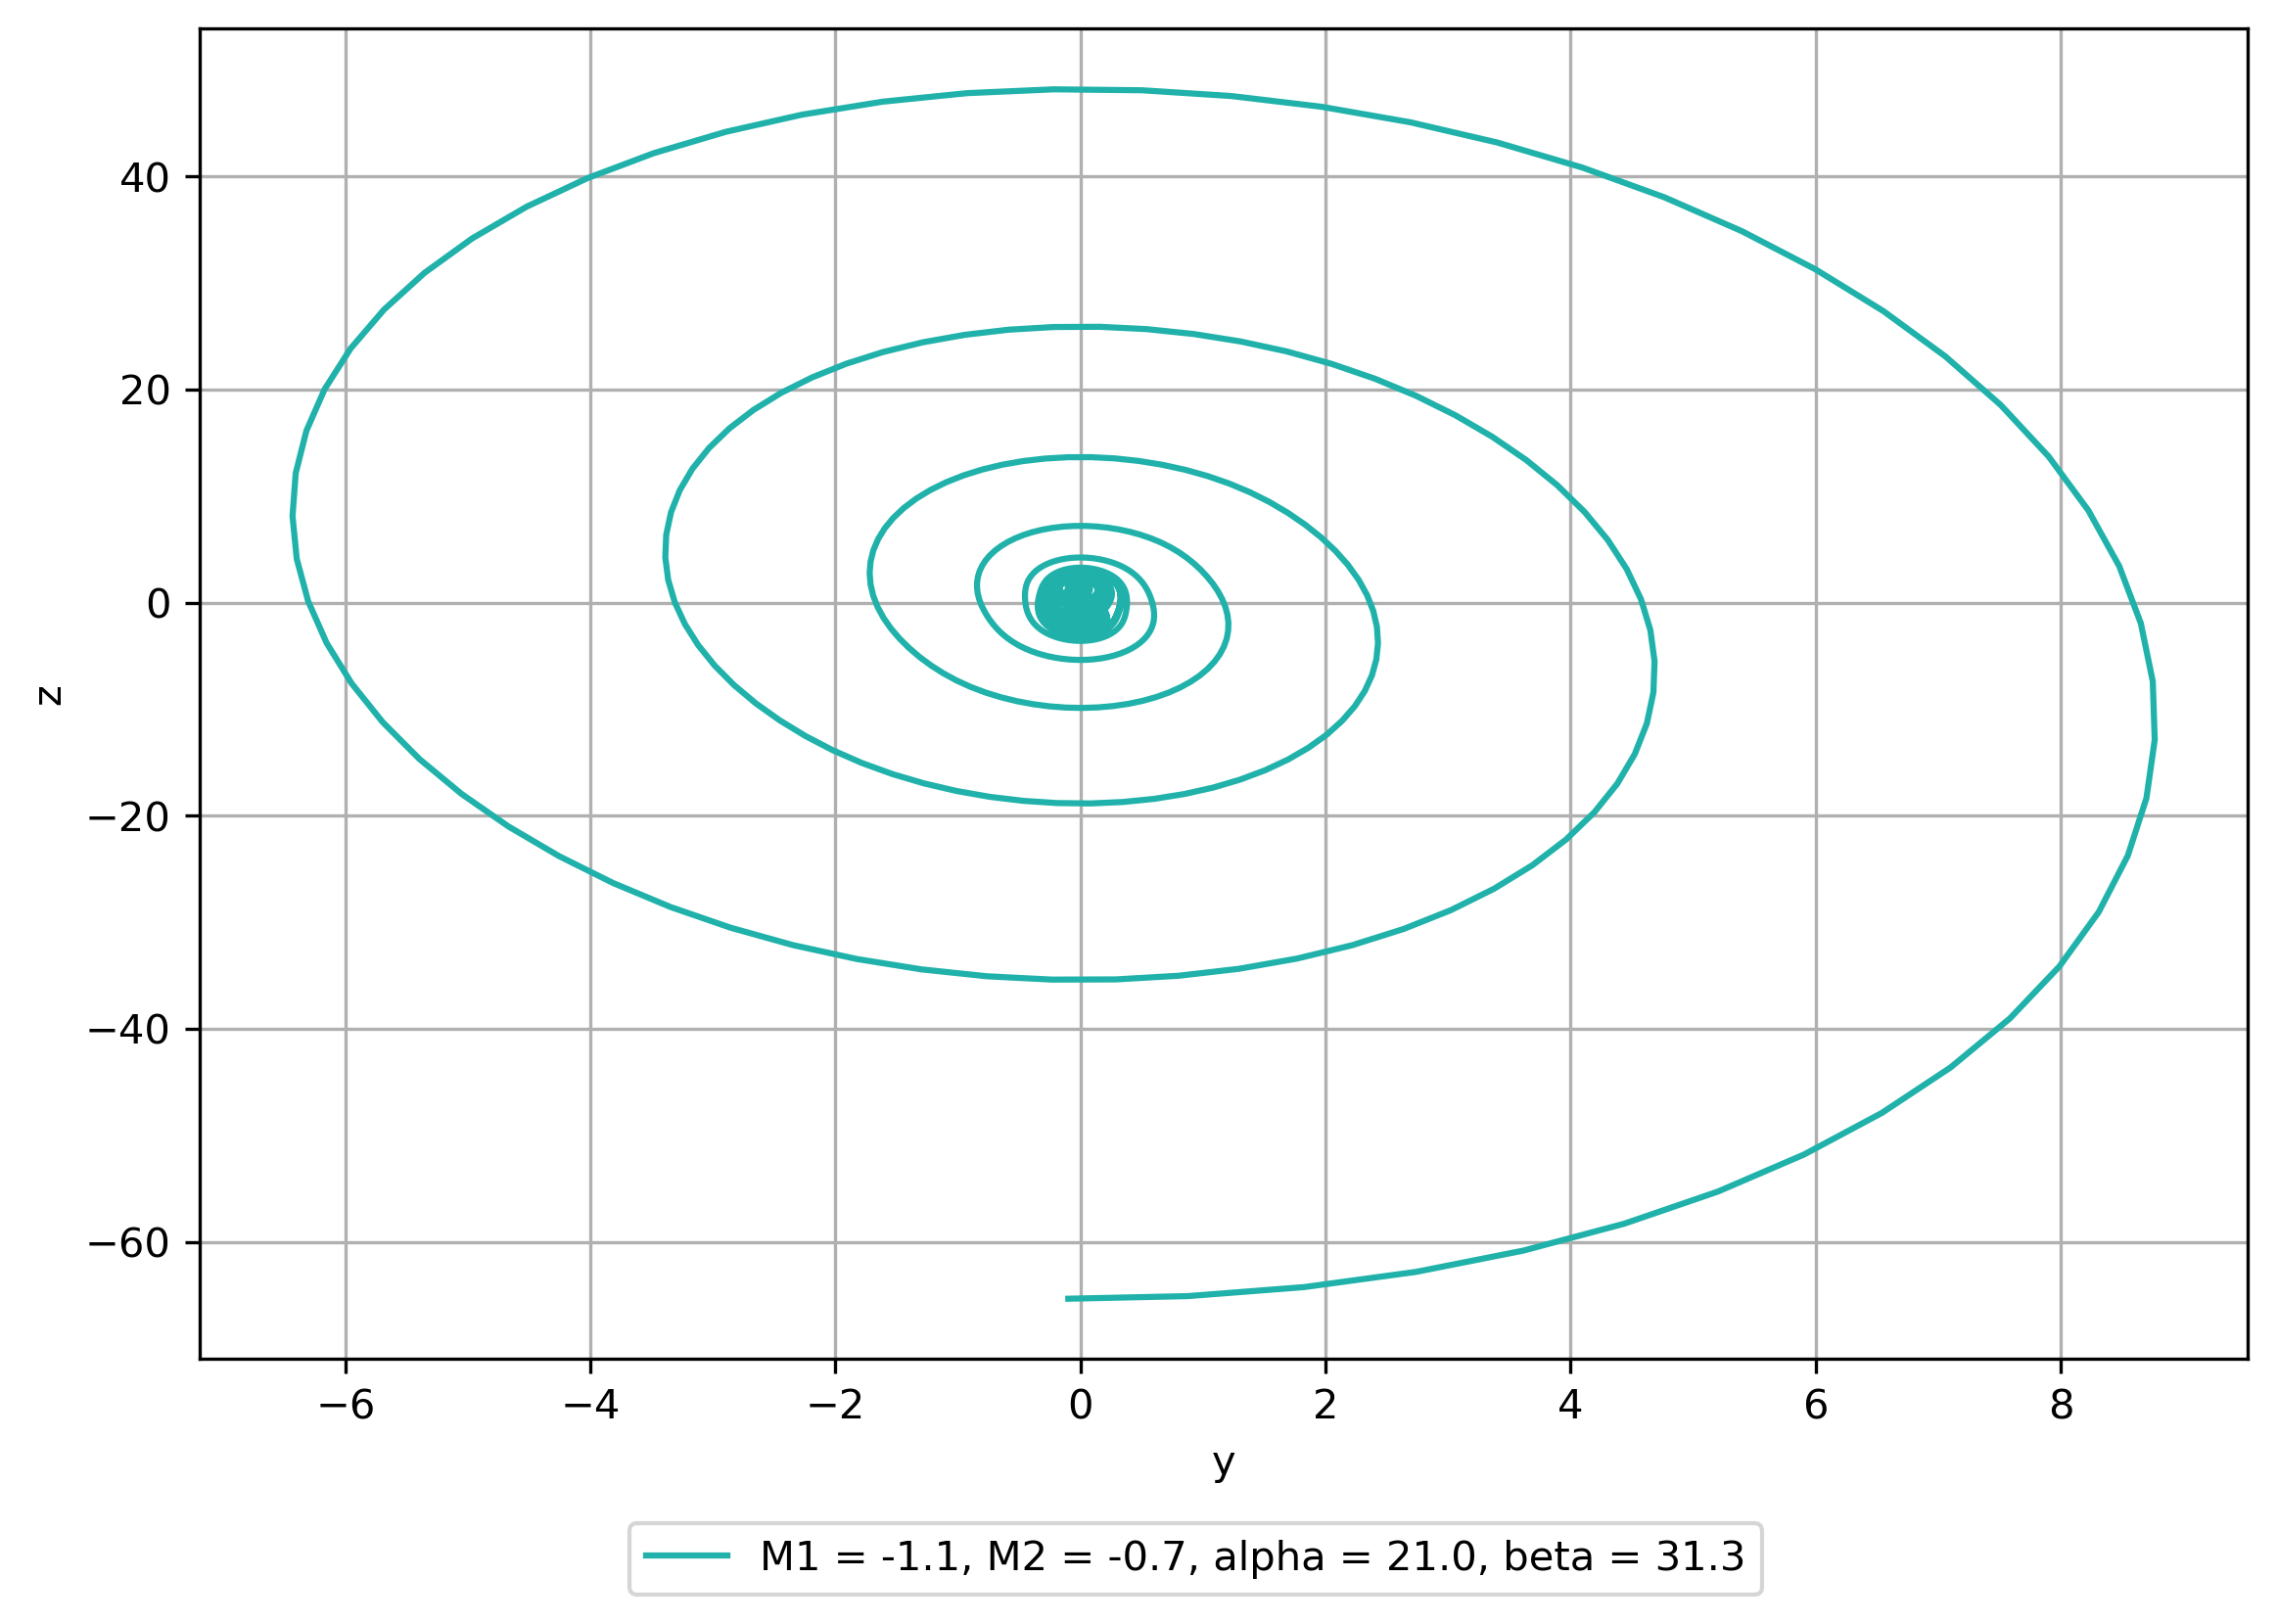
\includegraphics[width=0.3\textwidth]{attachments/fig.1.4.y-z.png}
				}
				\caption{\textbf{Numerical calculation of Chua's circuit, 1st single attractor}}
				\label{fig.1.4}
			\end{figure*}

			\begin{figure*}[htbp]
				\centering
				\subfloat[Channel]{
				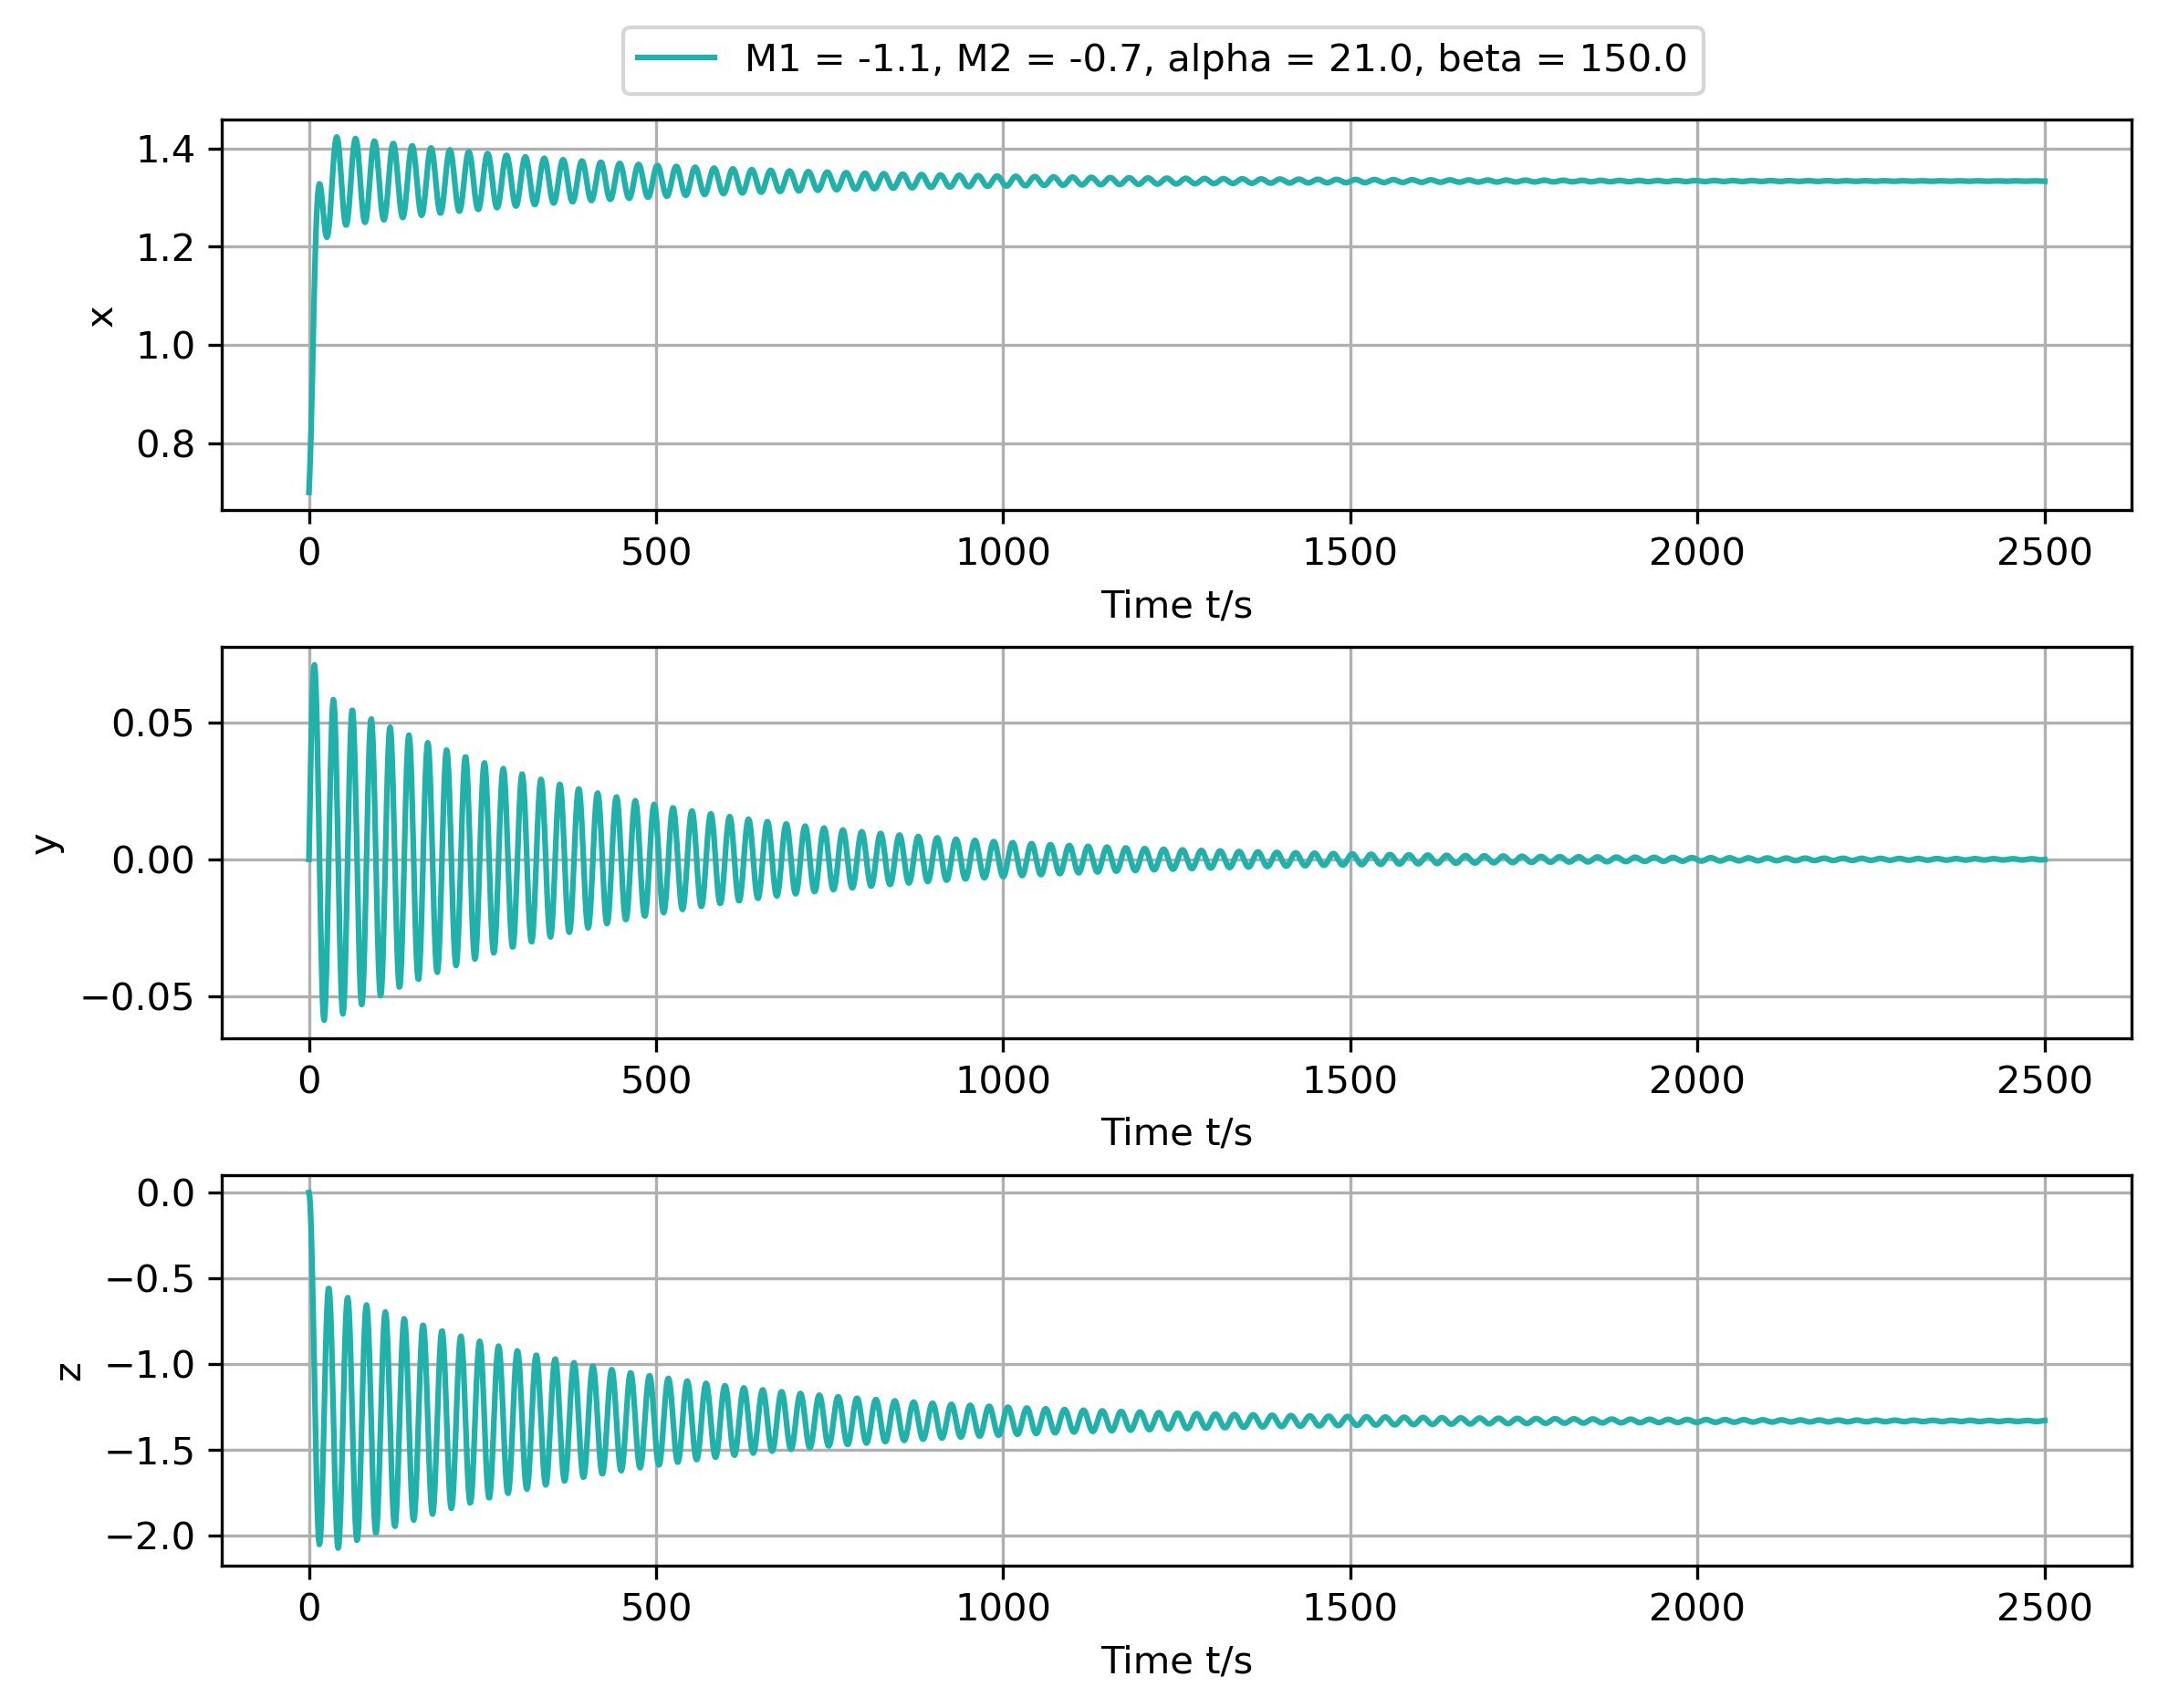
\includegraphics[width=0.3\textwidth]{attachments/fig.1.5.wave.png}
				}
				\subfloat[3d trace]{
				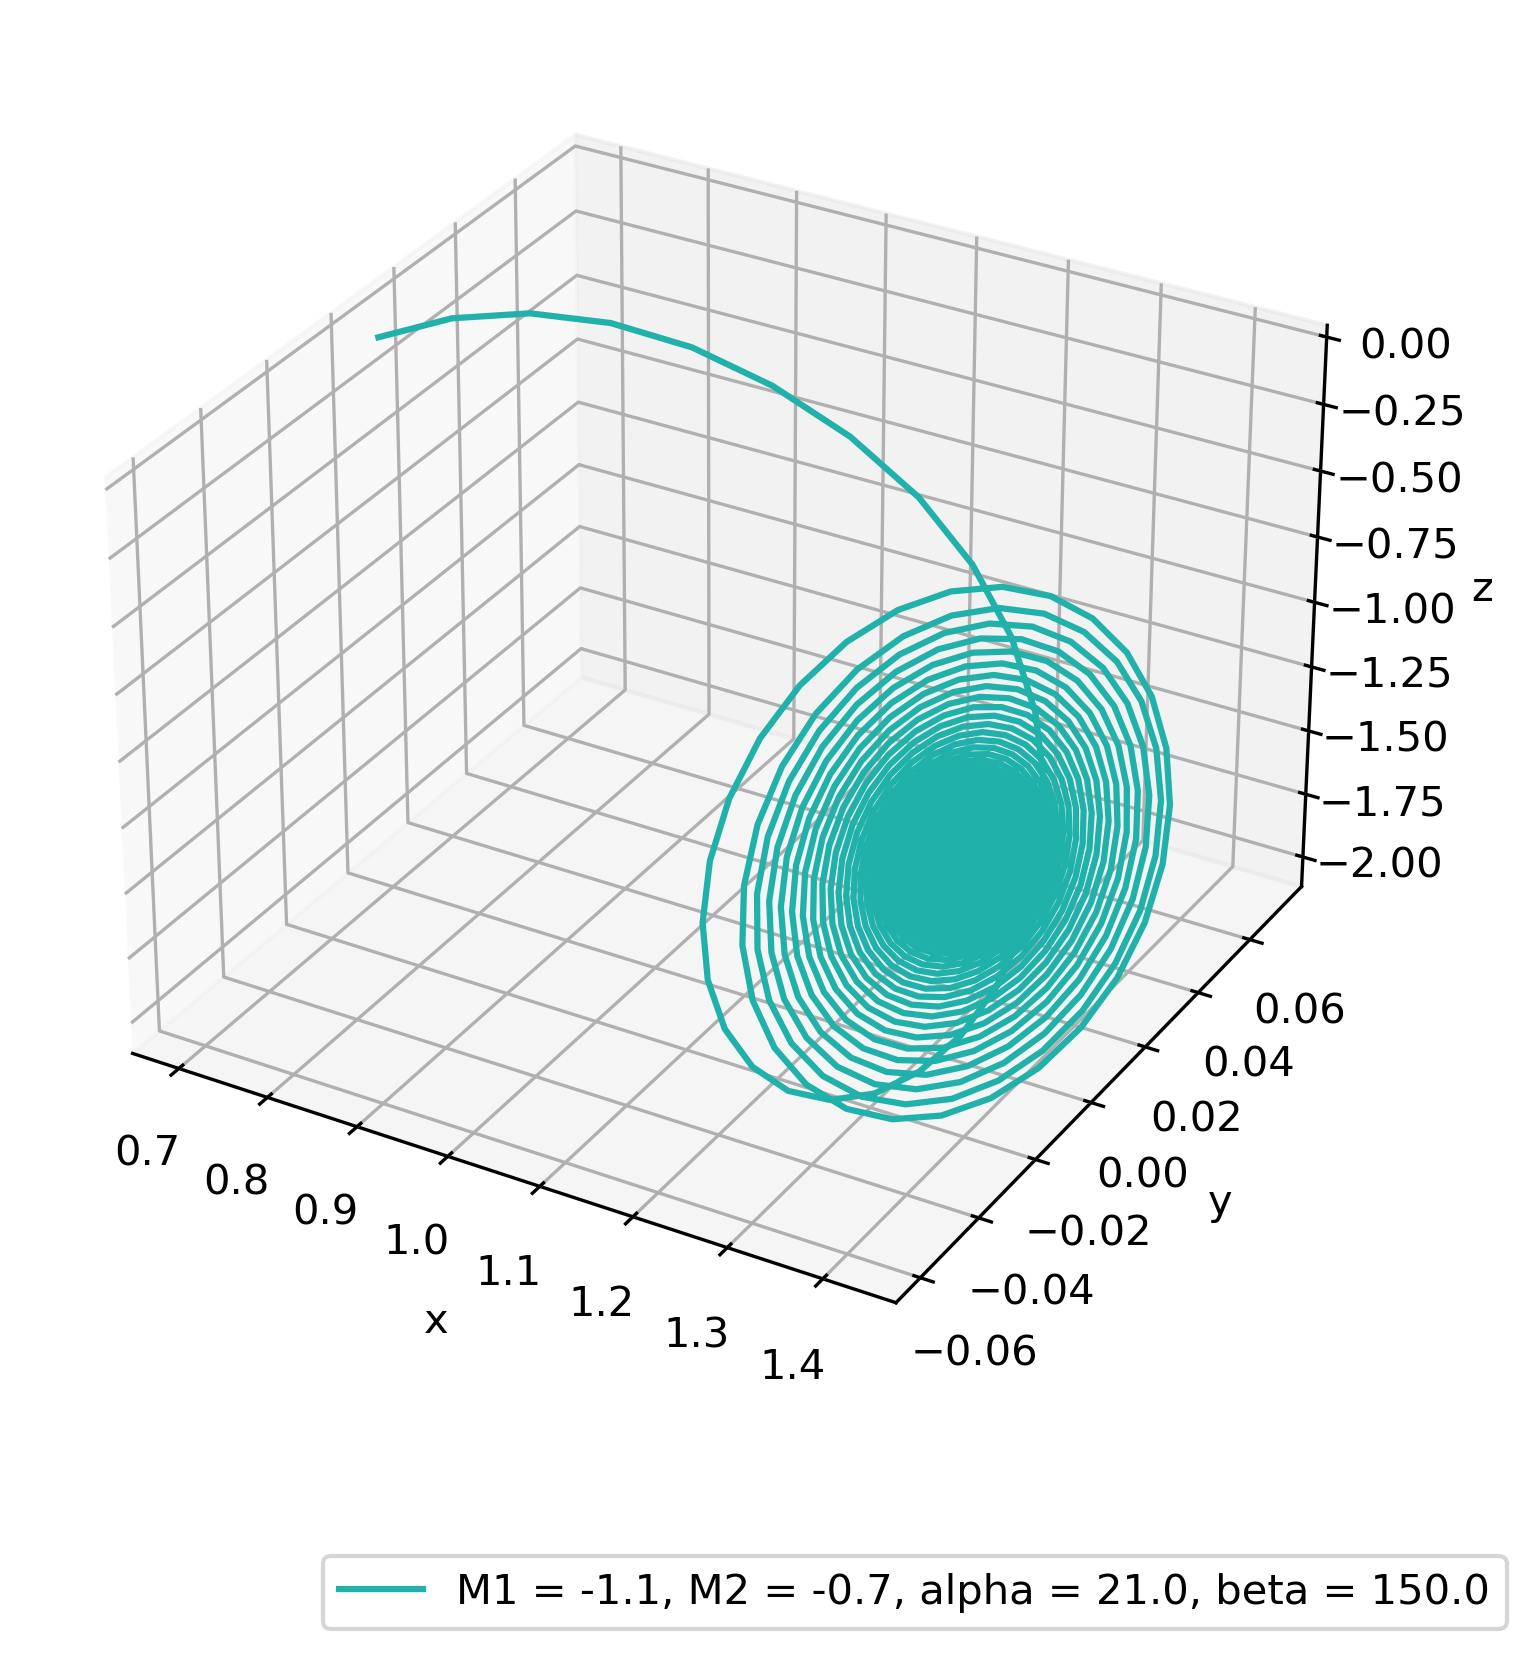
\includegraphics[width=0.3\textwidth]{attachments/fig.1.5.3d.png}
				}

				\subfloat[x-y plain]{
				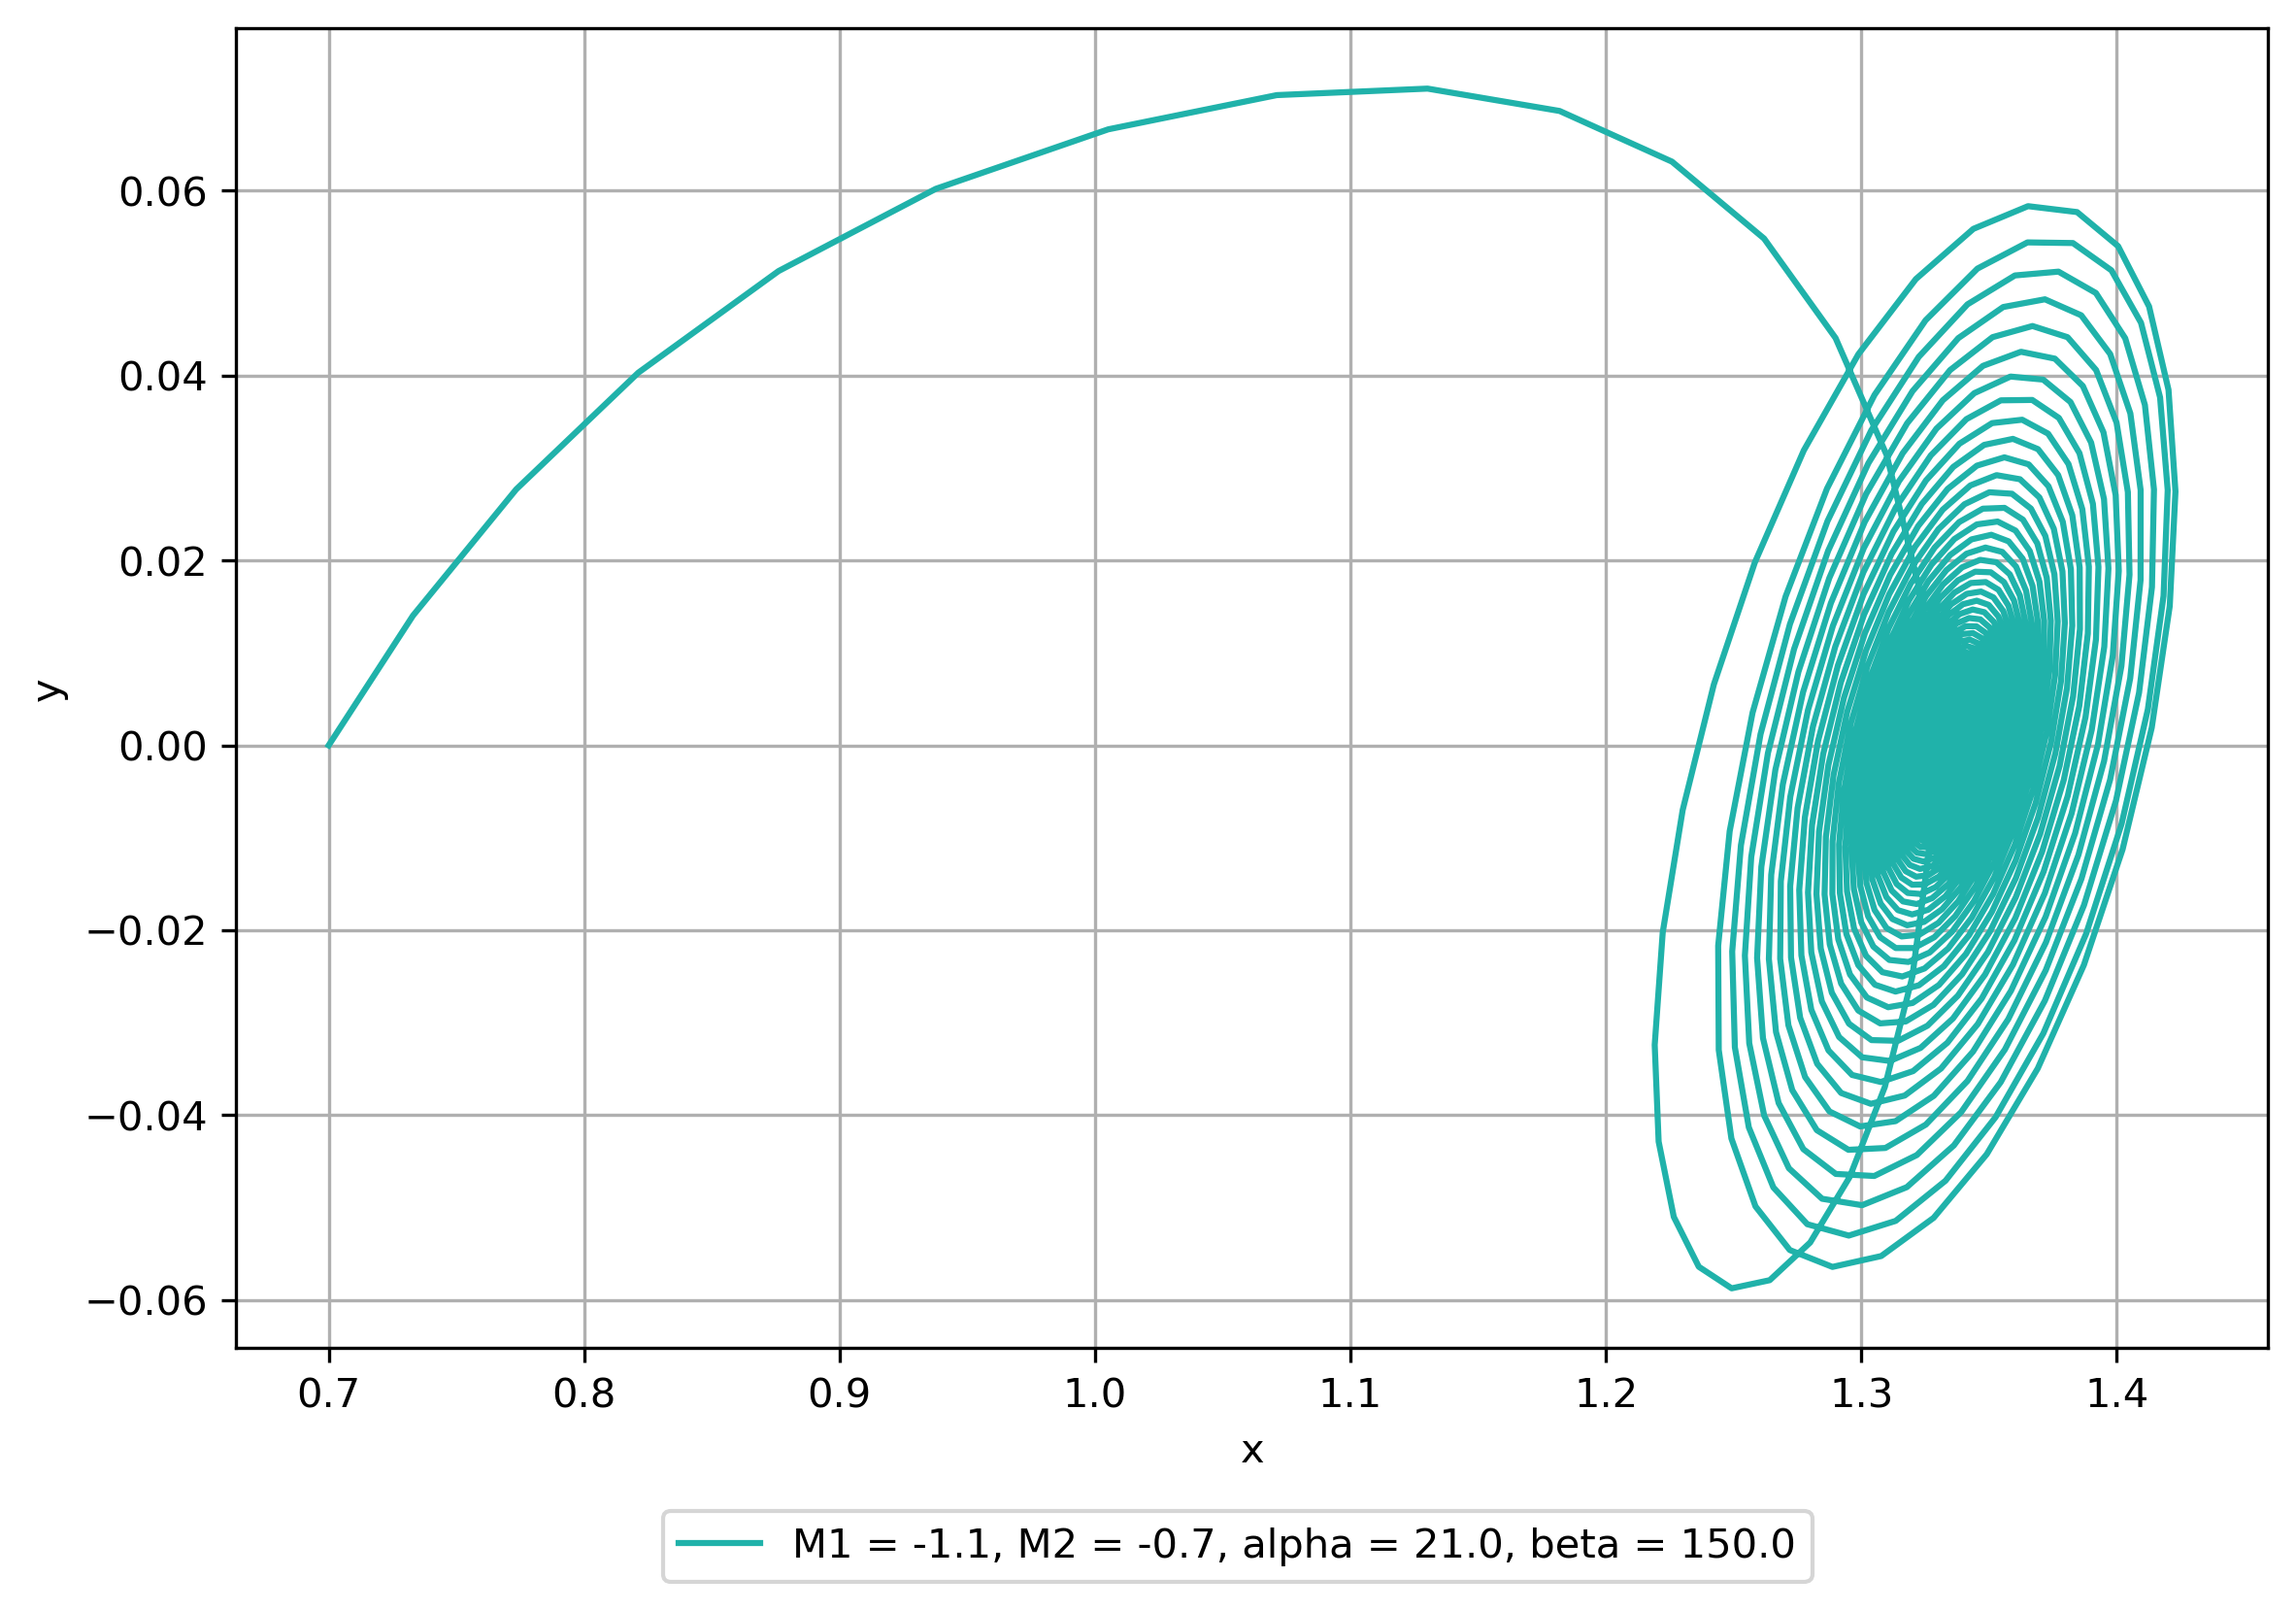
\includegraphics[width=0.3\textwidth]{attachments/fig.1.5.x-y.png}
				}
				\subfloat[x-z plain]{
				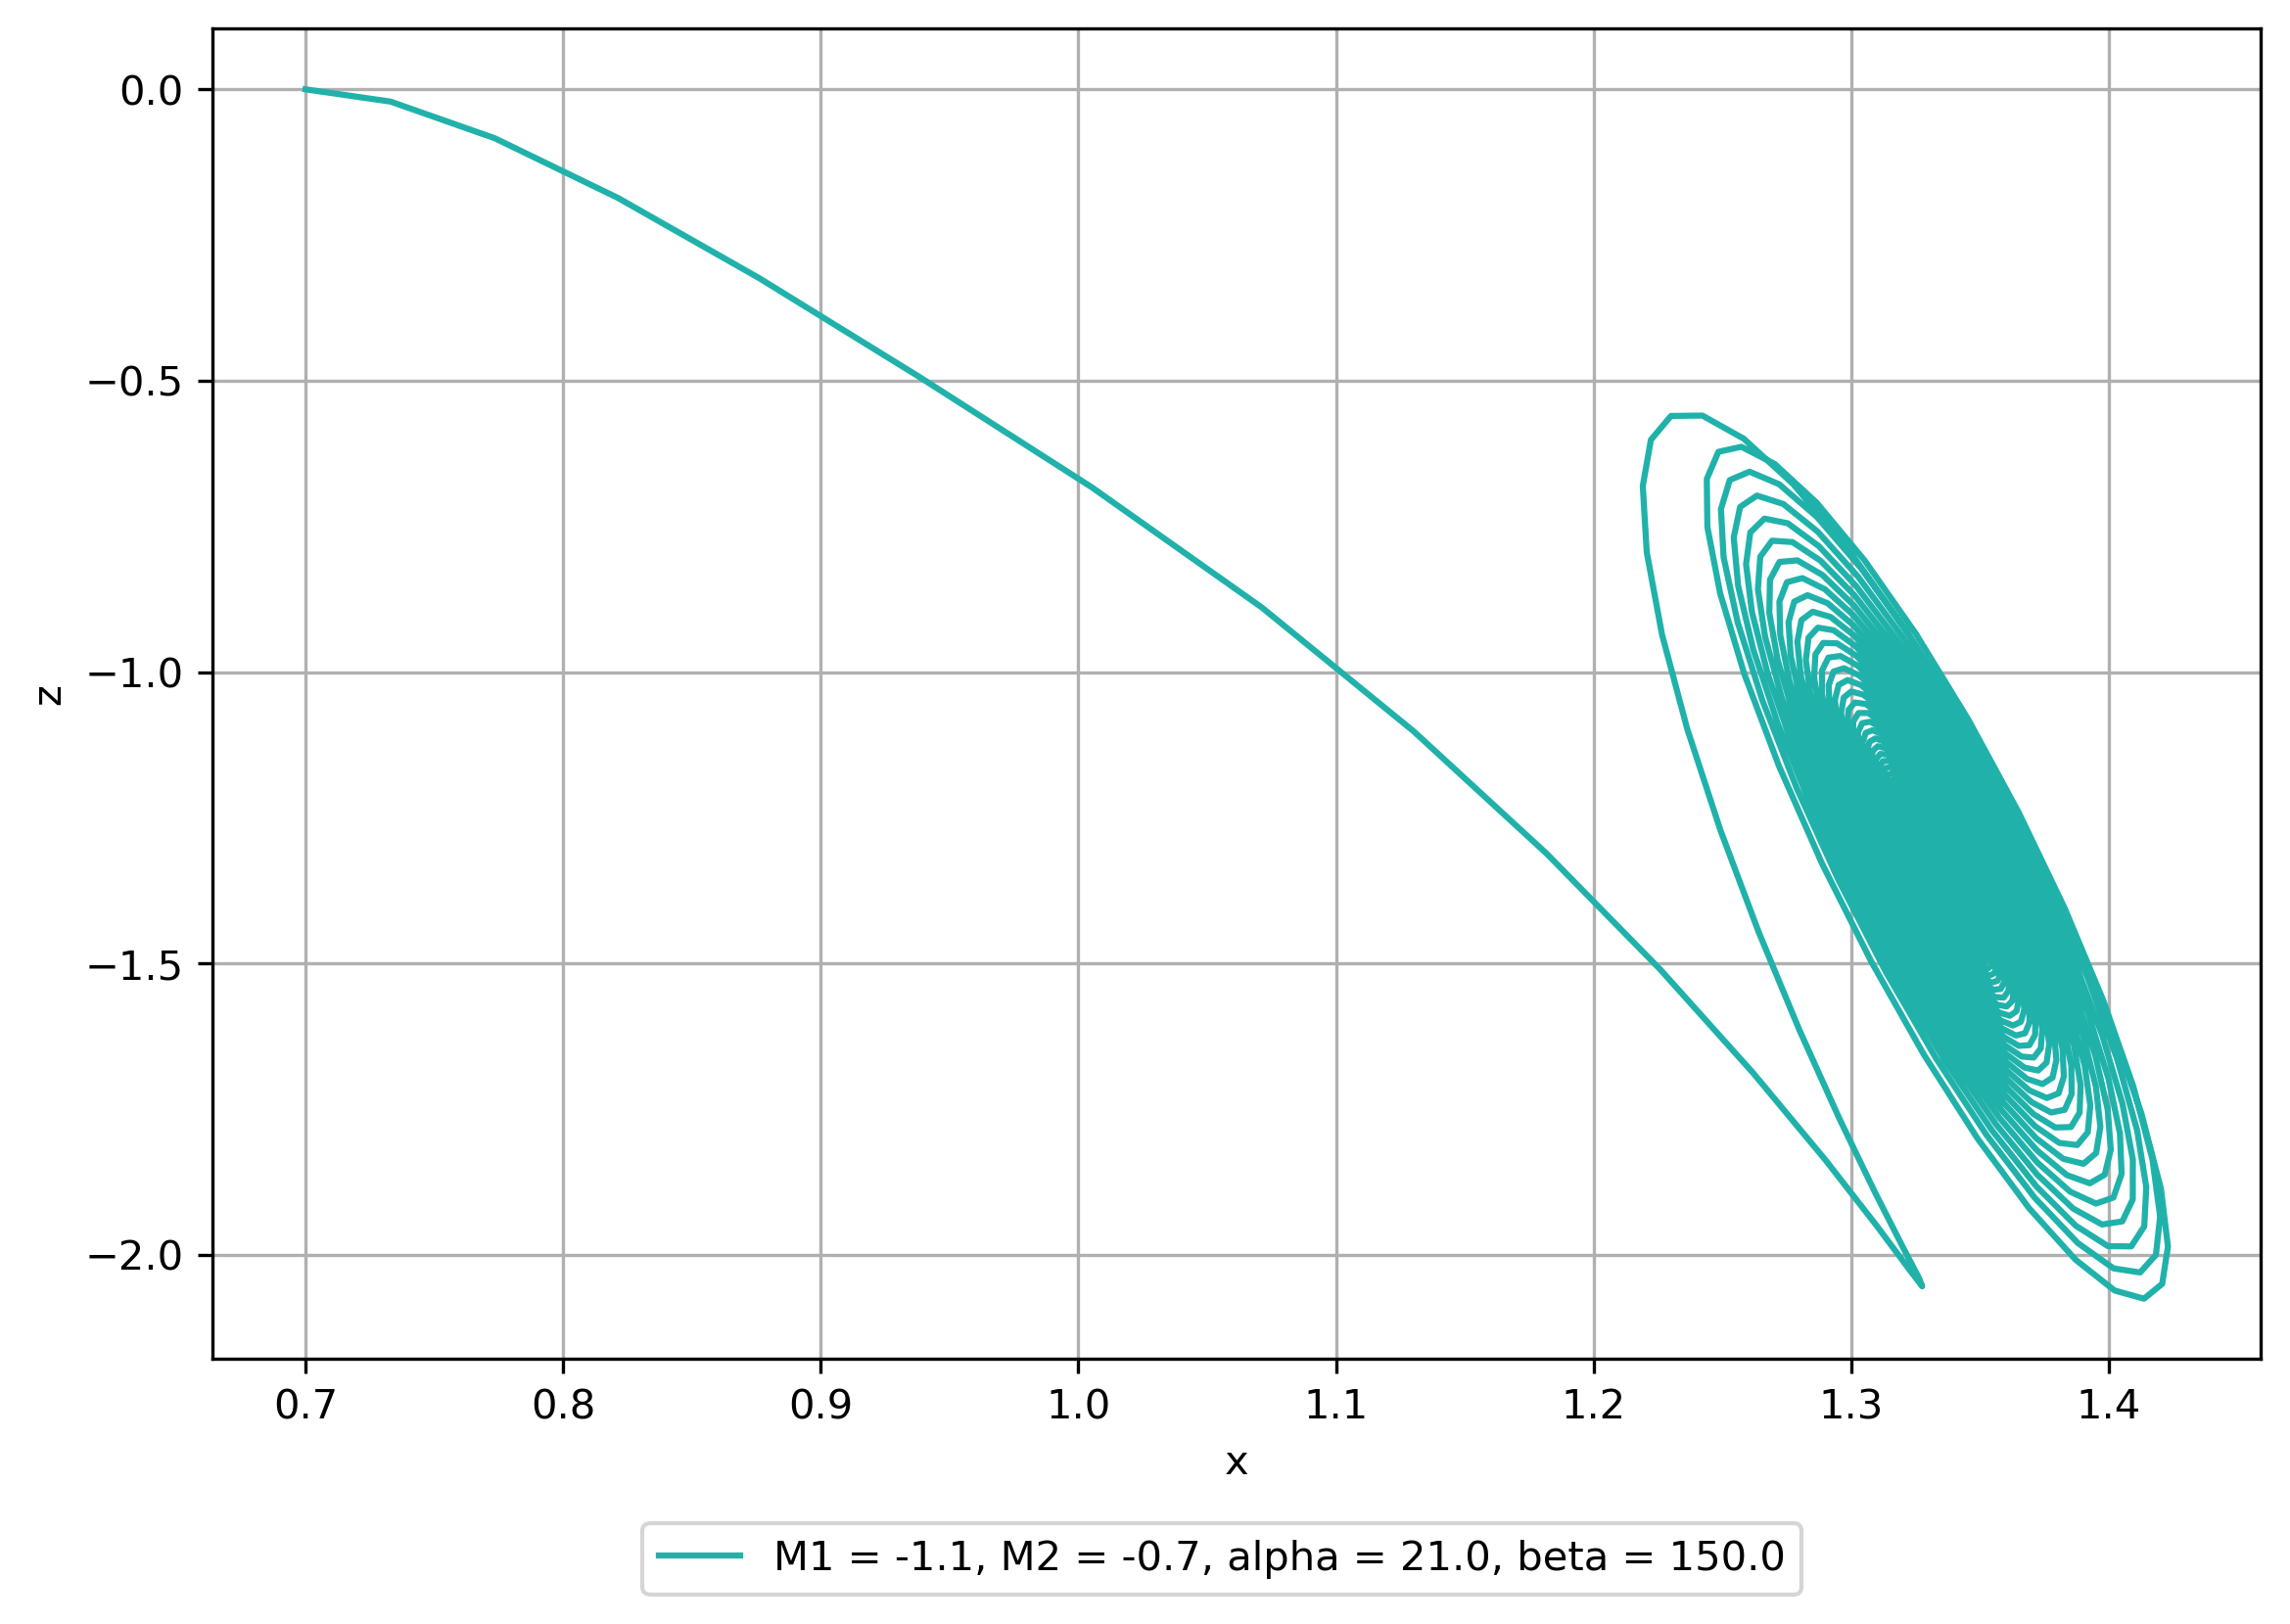
\includegraphics[width=0.3\textwidth]{attachments/fig.1.5.x-z.png}
				}
				\subfloat[y-z plain]{
				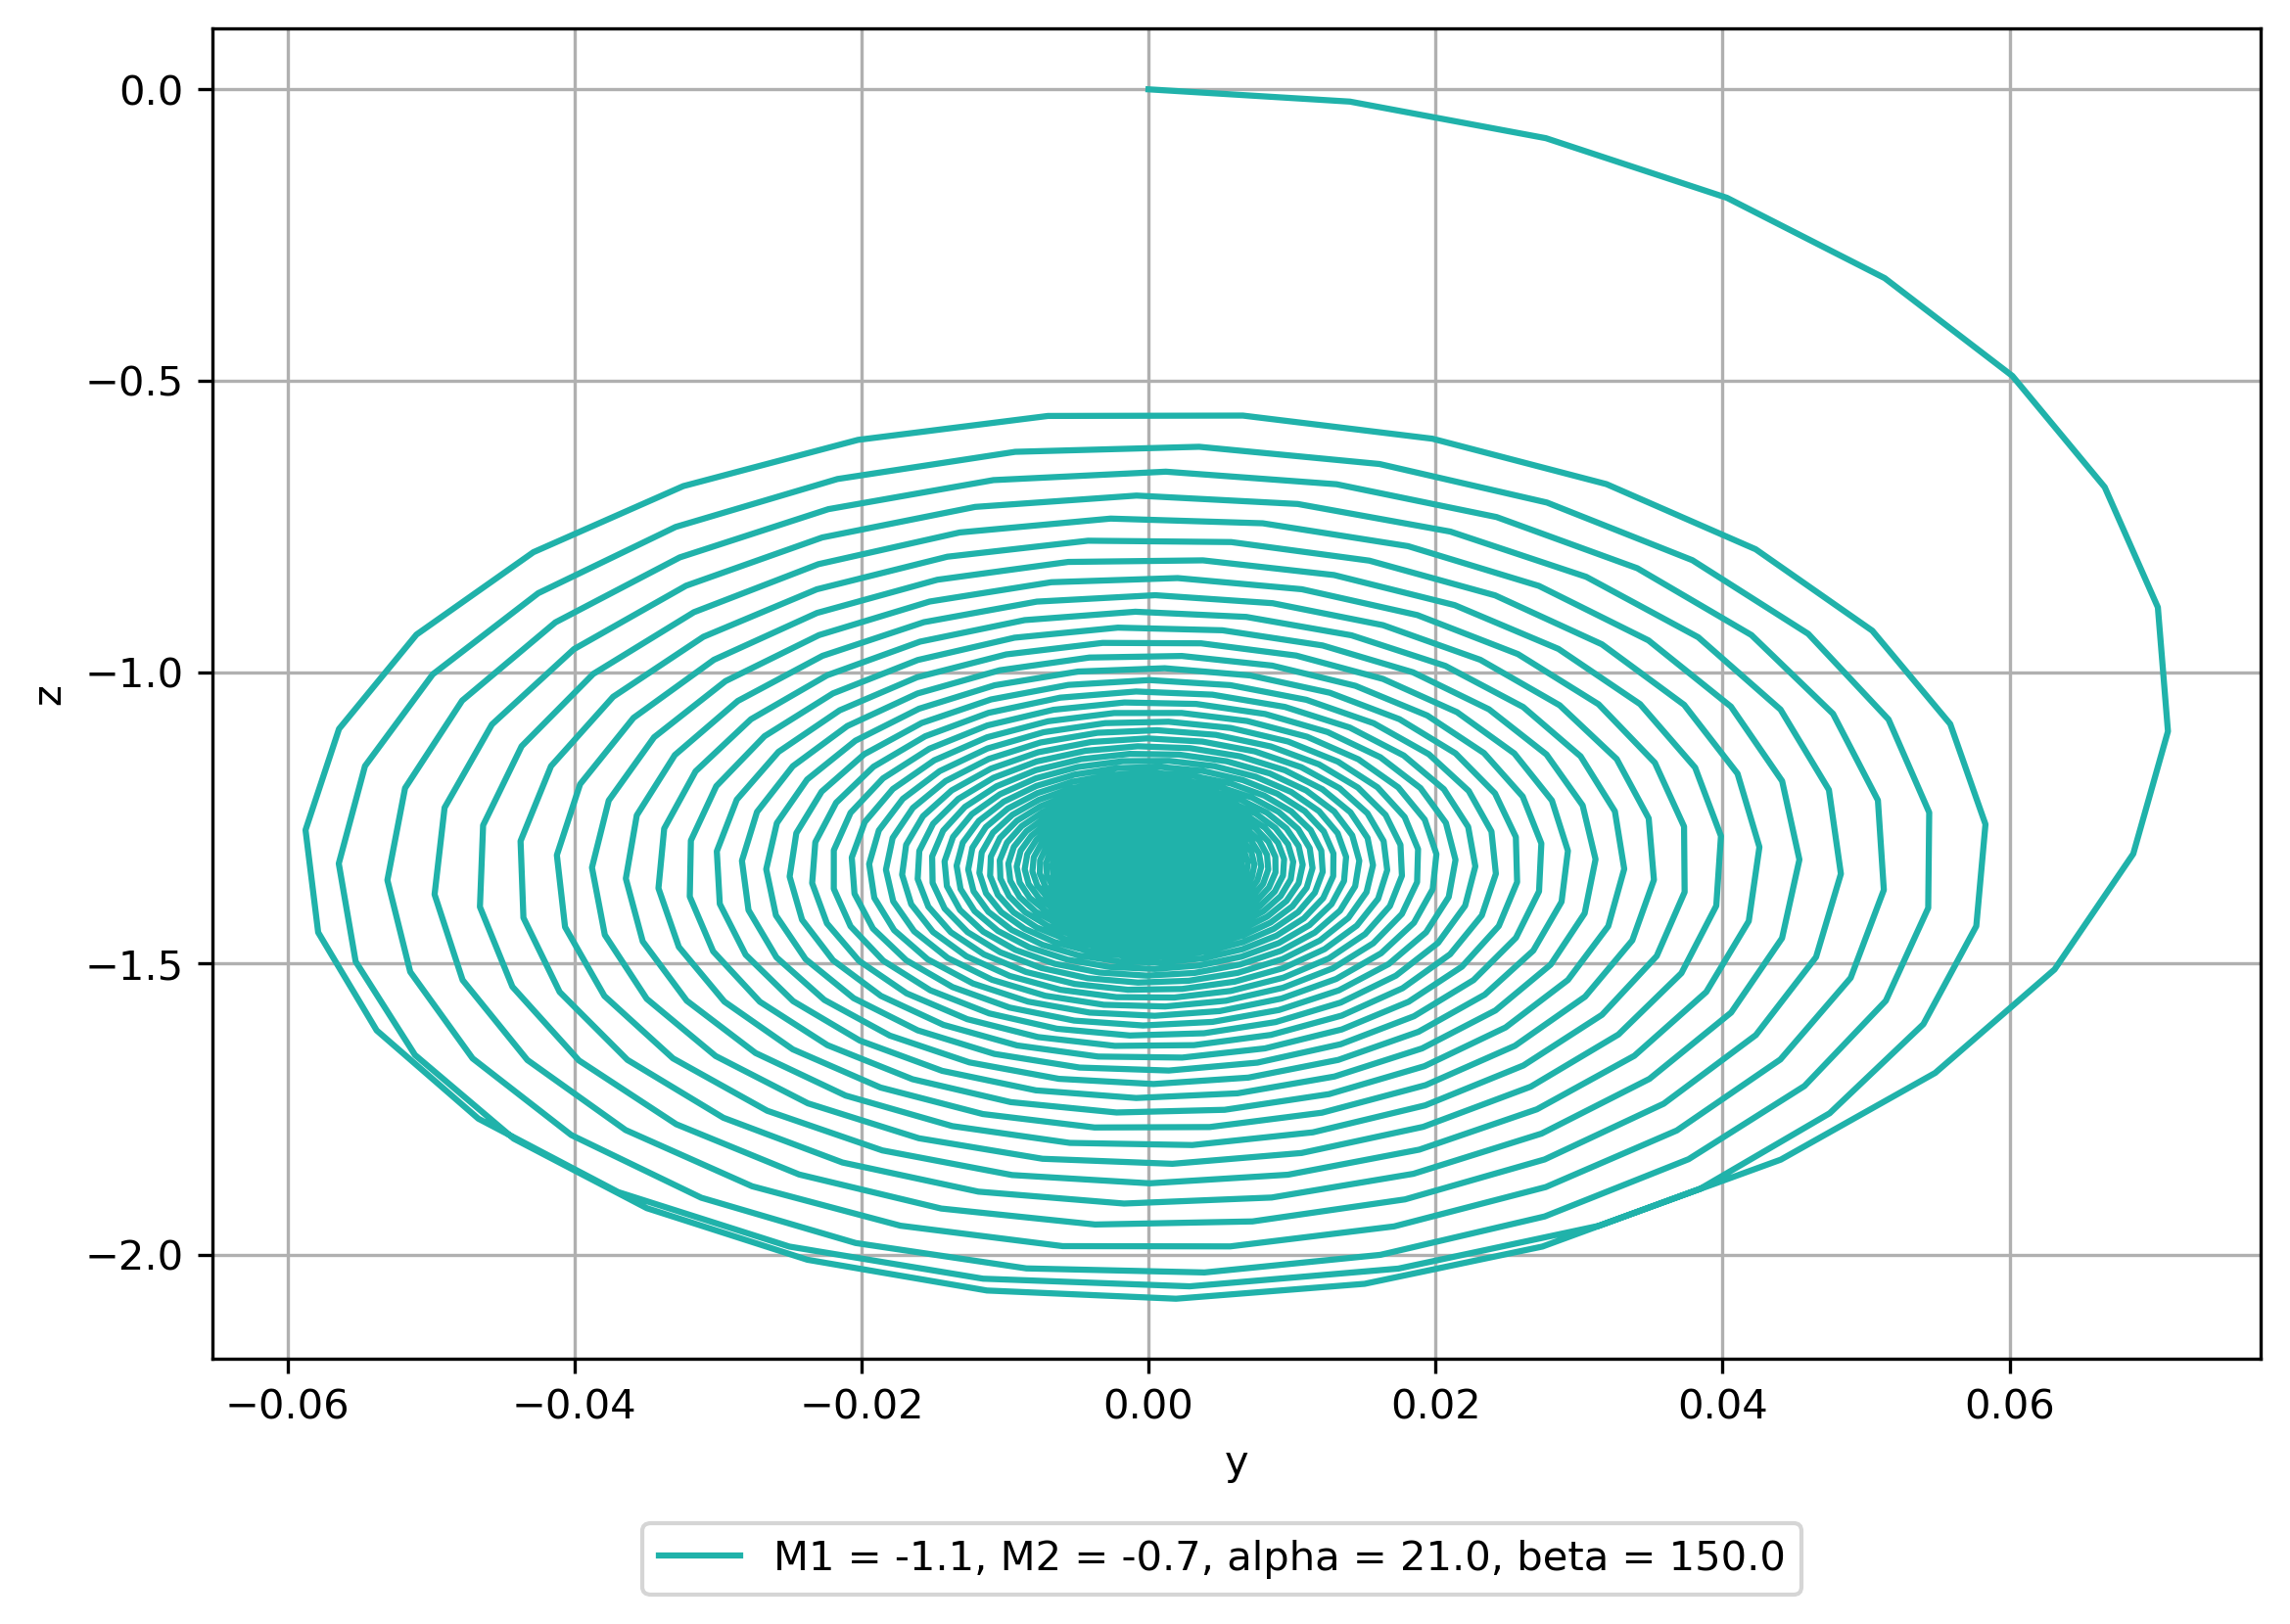
\includegraphics[width=0.3\textwidth]{attachments/fig.1.5.y-z.png}
				}
				\caption{\textbf{Numerical calculation of Chua's circuit, 2nd single attractor}}
				\label{fig.1.5}
			\end{figure*}
		
		\subsubsection{Simulation}
			Both circuits introduced previously were built and run on the Multisim simulation platform. 
			For the circuit illustrated in \ref{fig.1.1}, all five chaotic oscillation patterns can be obtained (Fig. \ref{fig.2.1}).
			However, for the circuit illustrated in \ref{fig.1.2}, we could only obtained four patterns (Fig. \ref{fig.2.2}).
			After the occurrence of the first single attractor, as we continued to increase the resistance value, the attractor was keeping shrinking, so the pattern of second single attractor never appeared and was missing.
			We hypothesis that the circuit illustrated in \ref{fig.1.1}, which adopted Kennedy's two op-amp realization\autocite{prakashChuaCircuitParadigm2020}, is more robust and effective than the second one.

			The parameters of different chaotic oscillation patterns are summarized in the Supplementary Information.
			\begin{figure*}[htbp]
				\centering
				\subfloat[line]{
				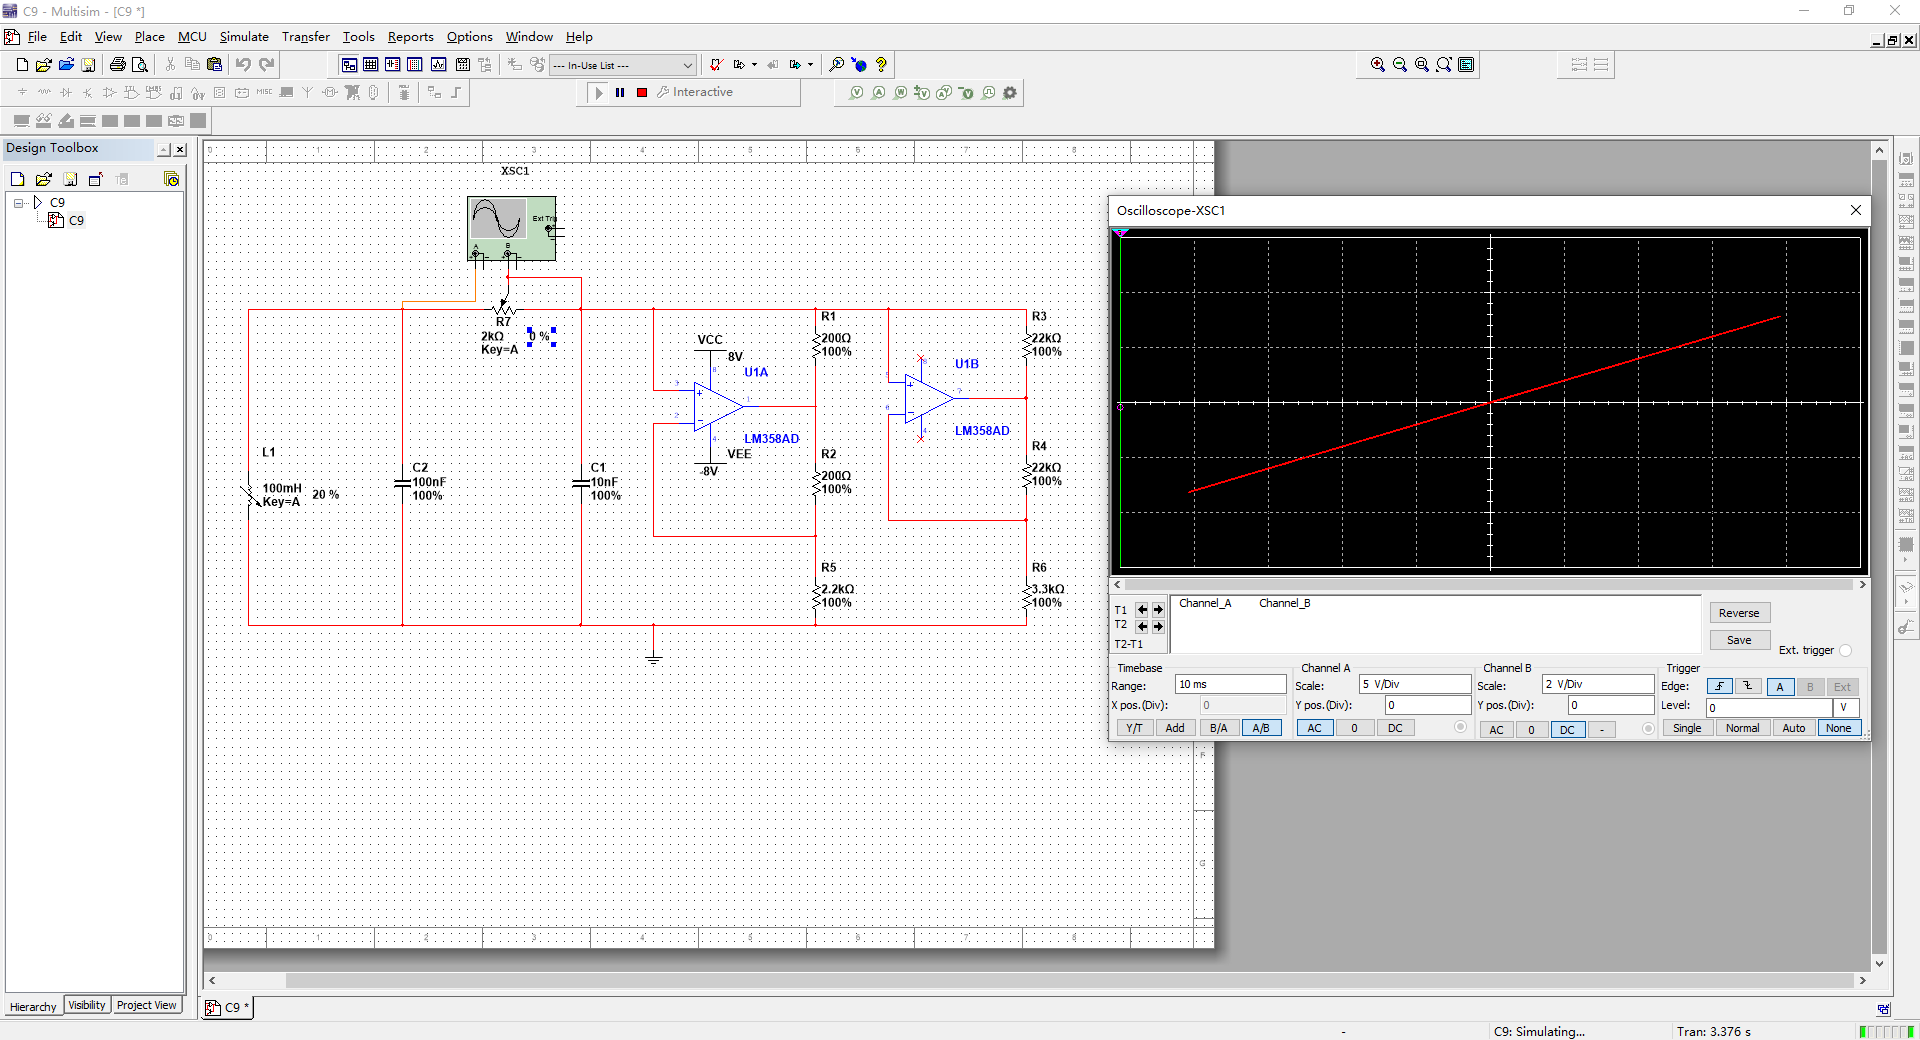
\includegraphics[width=0.3\textwidth]{attachments/fig.2.1.line.png}
				}
				\subfloat[limit ring]{
				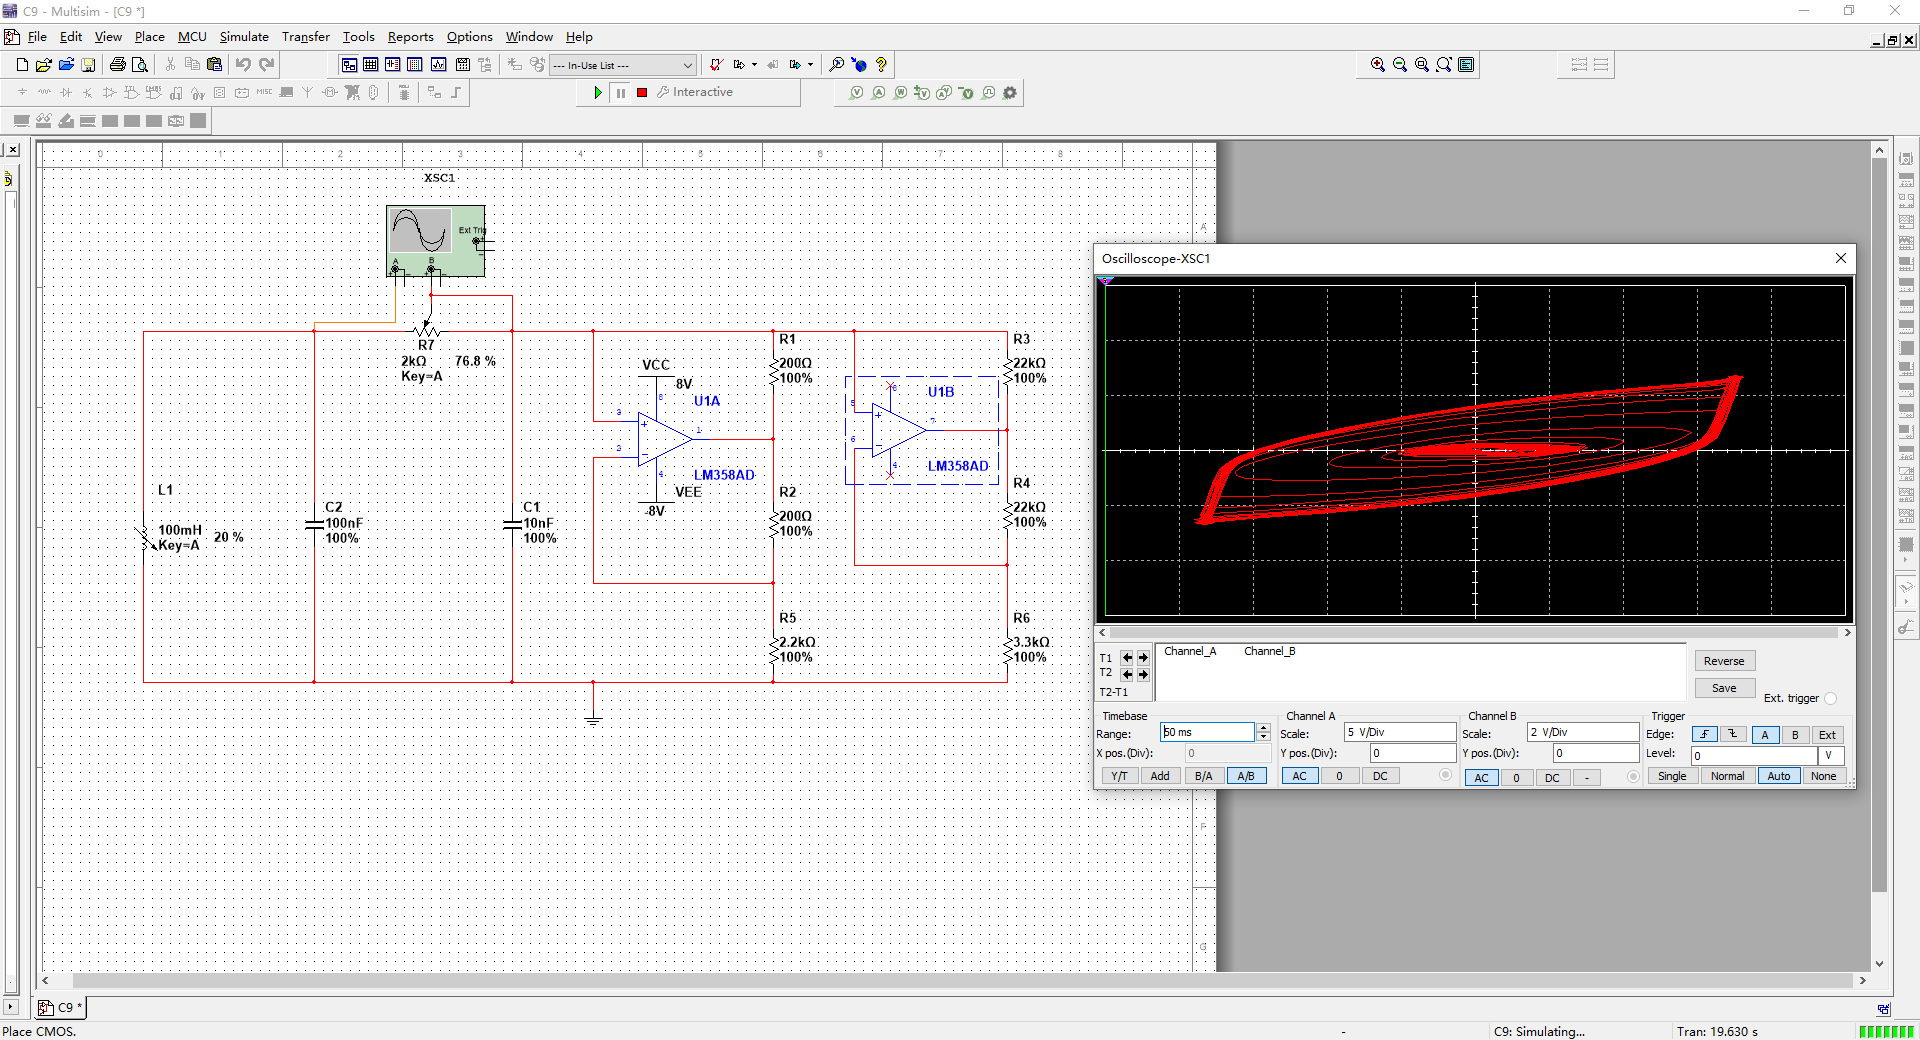
\includegraphics[width=0.3\textwidth]{attachments/fig.2.1.limit ring.png}
				}
				
				\subfloat[double attractors]{
				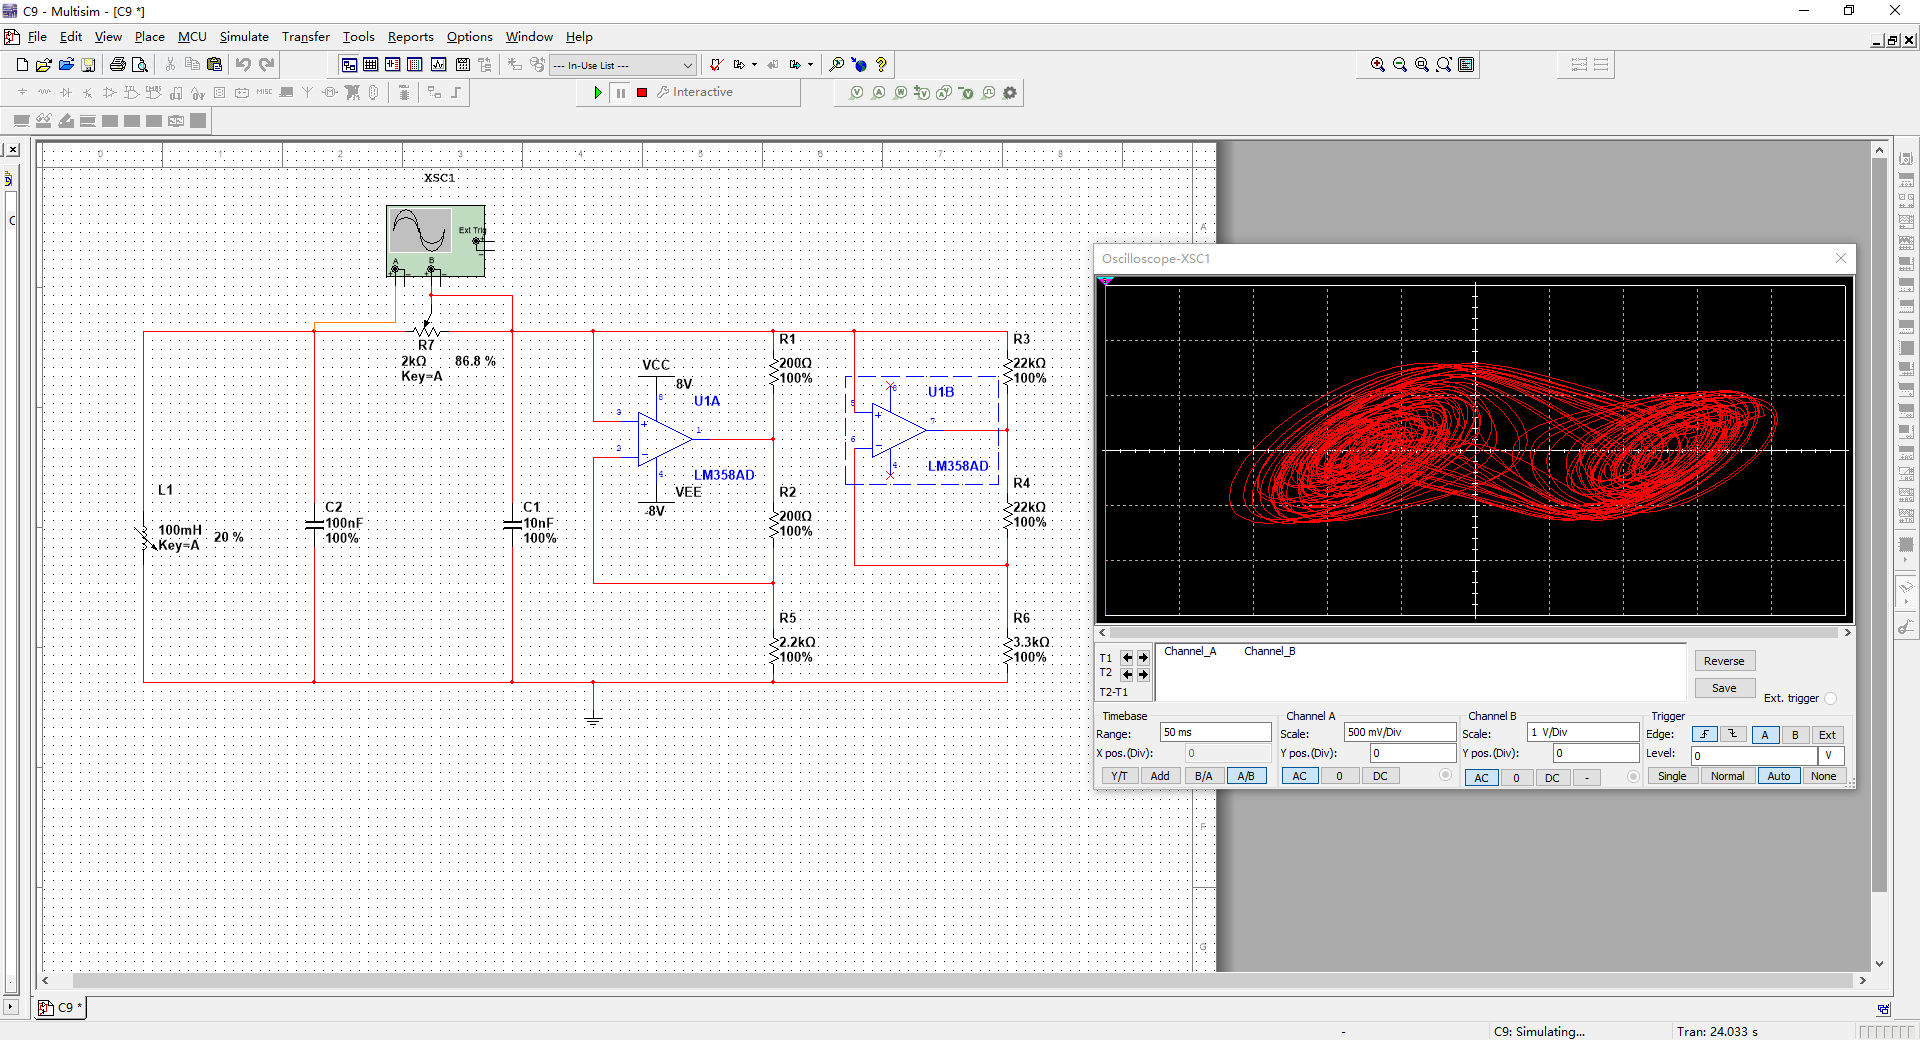
\includegraphics[width=0.3\textwidth]{attachments/fig.2.1.double attractors.png}
				}
				\subfloat[1st single attractor]{
				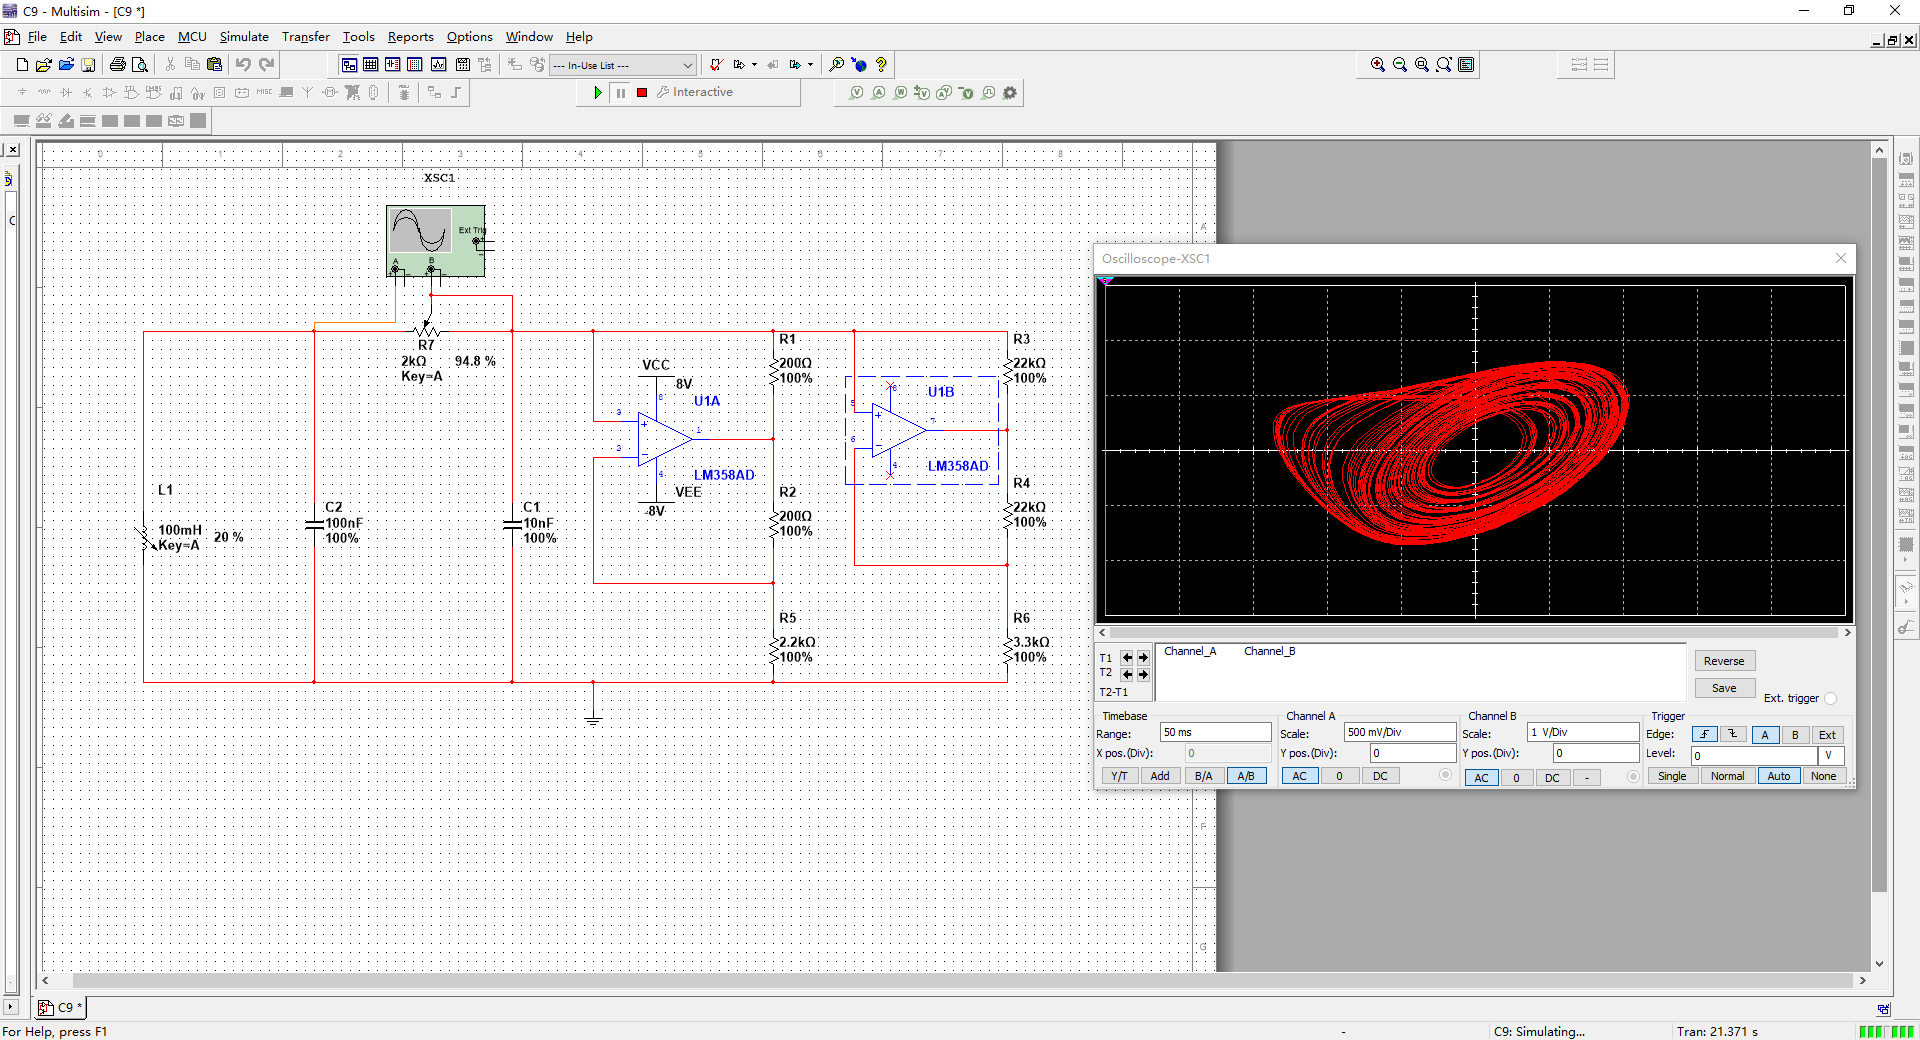
\includegraphics[width=0.3\textwidth]{attachments/fig.2.1.1st.png}
				}
				\subfloat[2nd single attractor]{
				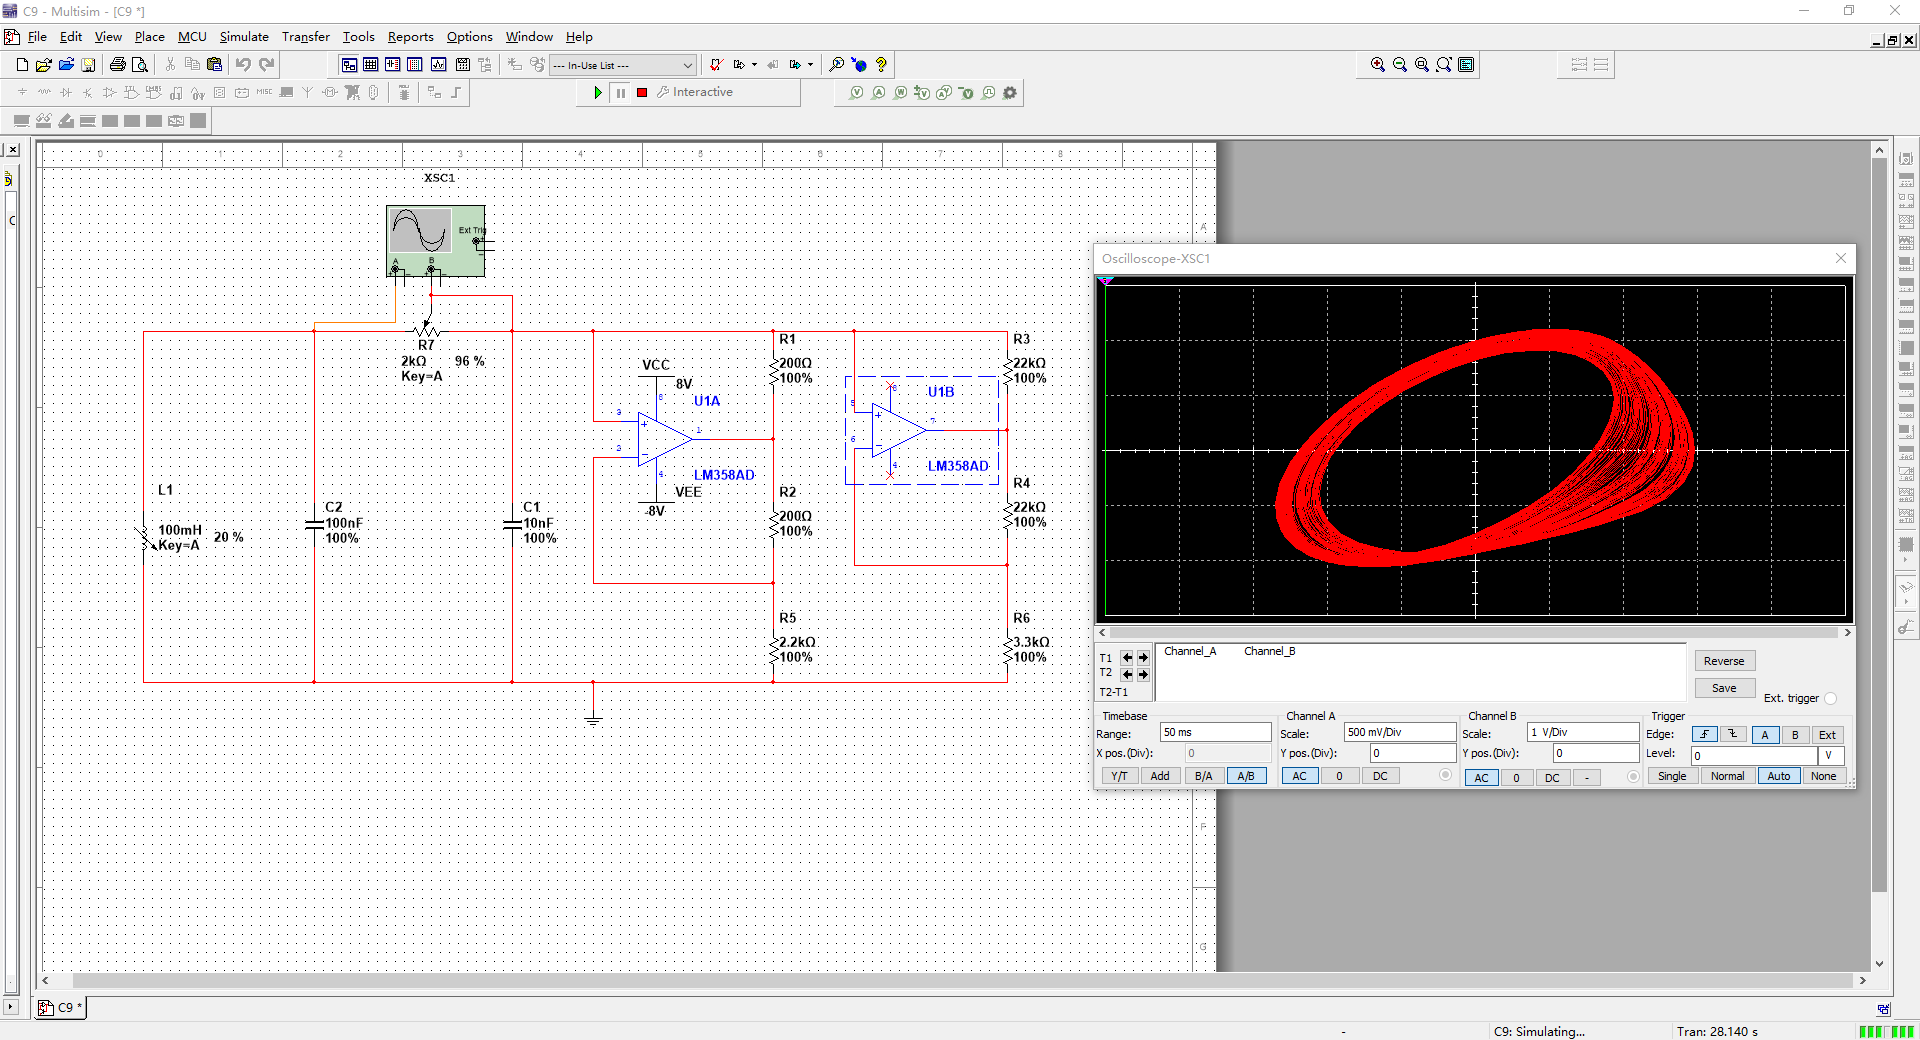
\includegraphics[width=0.3\textwidth]{attachments/fig.2.1.2nd.png}
				}
				\caption{\textbf{Chua's circuit I, simulation results}}
				\label{fig.2.1}
			\end{figure*}
		
			\begin{figure*}[htbp]
				\centering
				\subfloat[line]{
				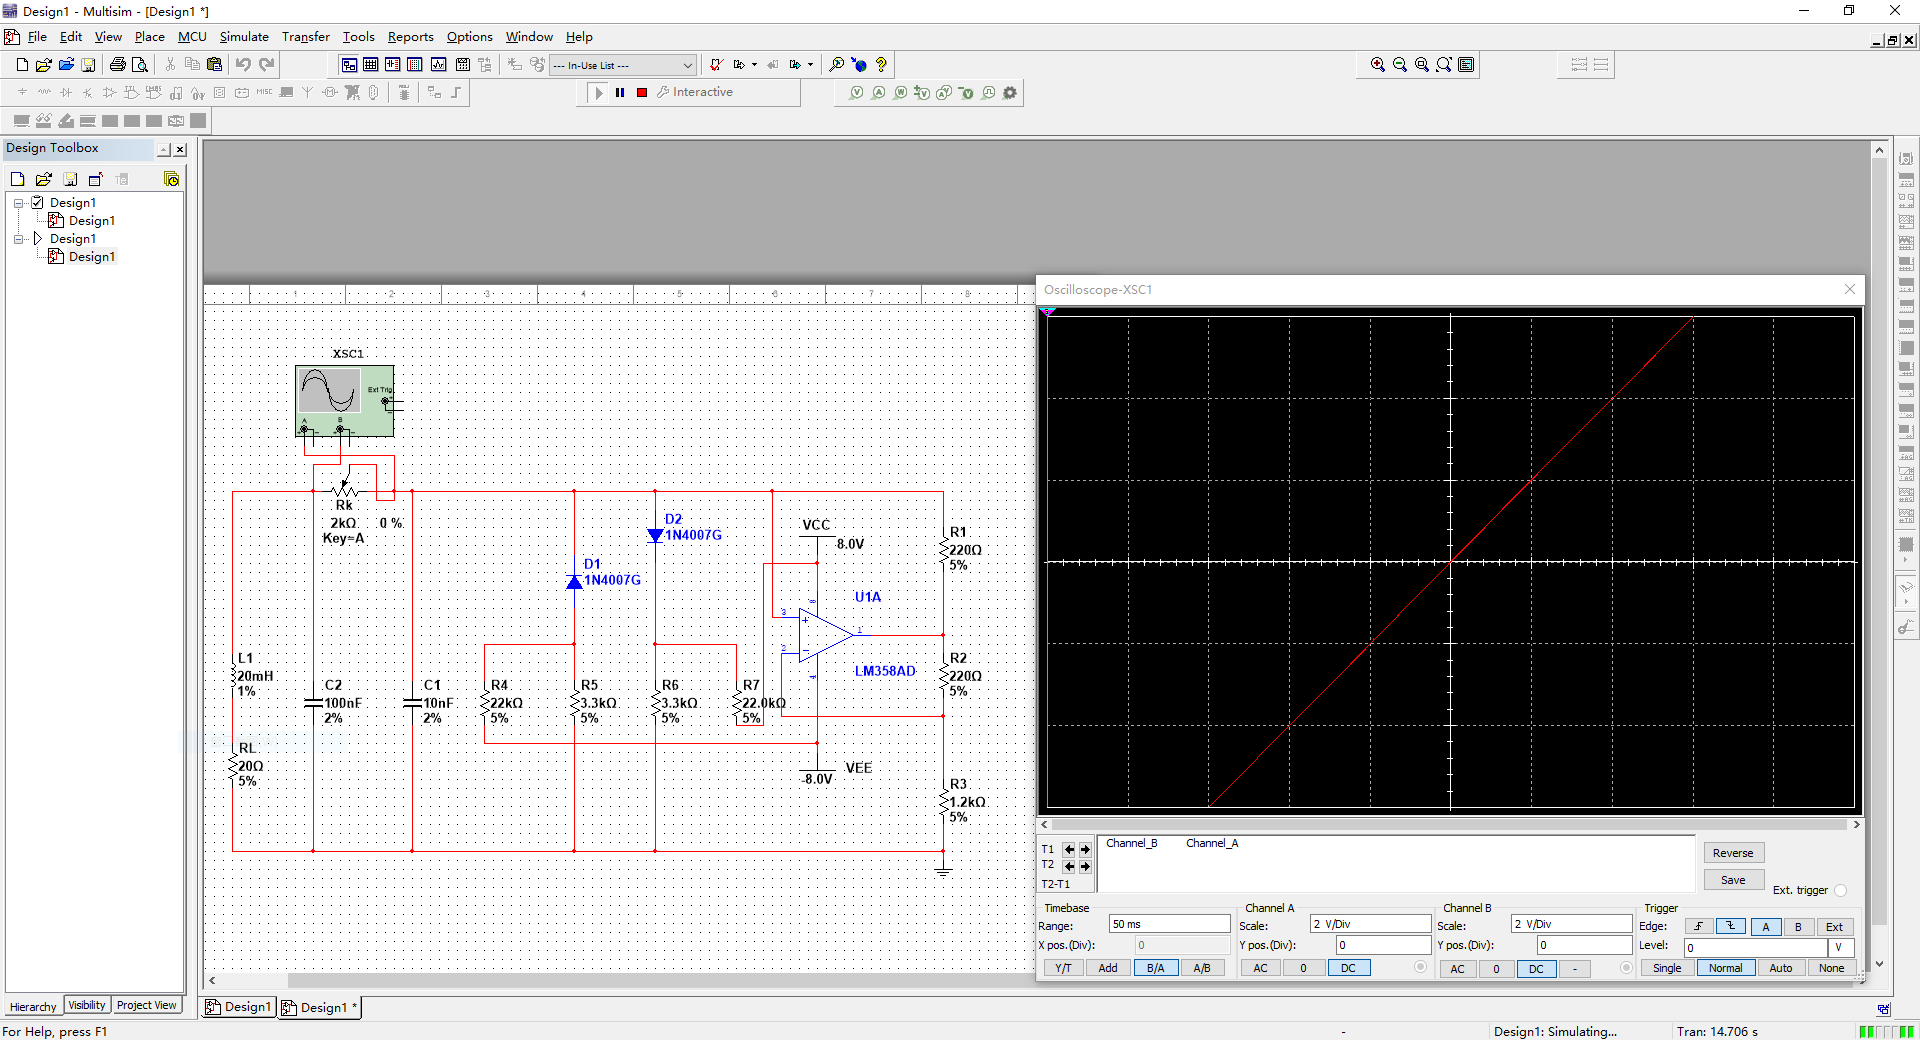
\includegraphics[width=0.3\textwidth]{attachments/fig.2.2.line.png}
				}
				\subfloat[limit ring]{
				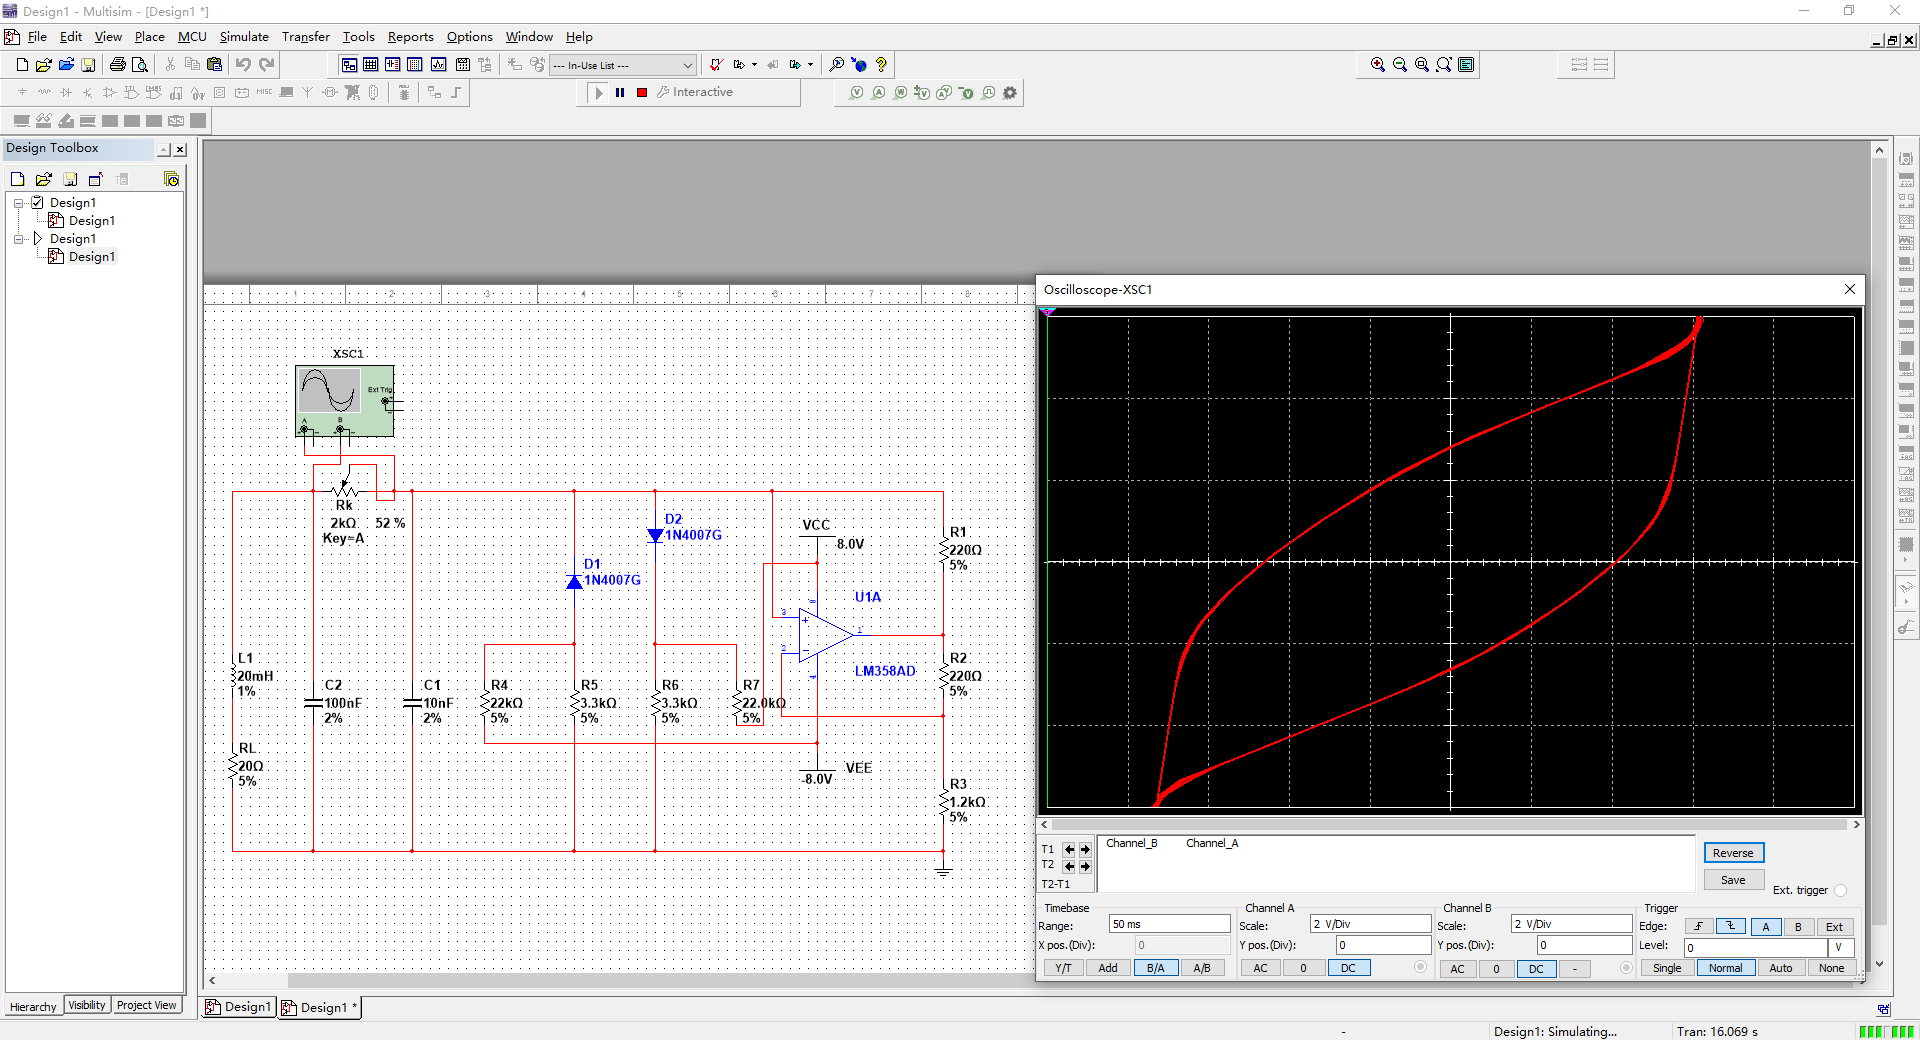
\includegraphics[width=0.3\textwidth]{attachments/fig.2.2.limit ring.png}
				}

				\subfloat[double attractors]{
				\includegraphics[width=0.3\textwidth]{attachments/fig.2.2.double attractors.png}
				}
				\subfloat[1st single attractor]{
				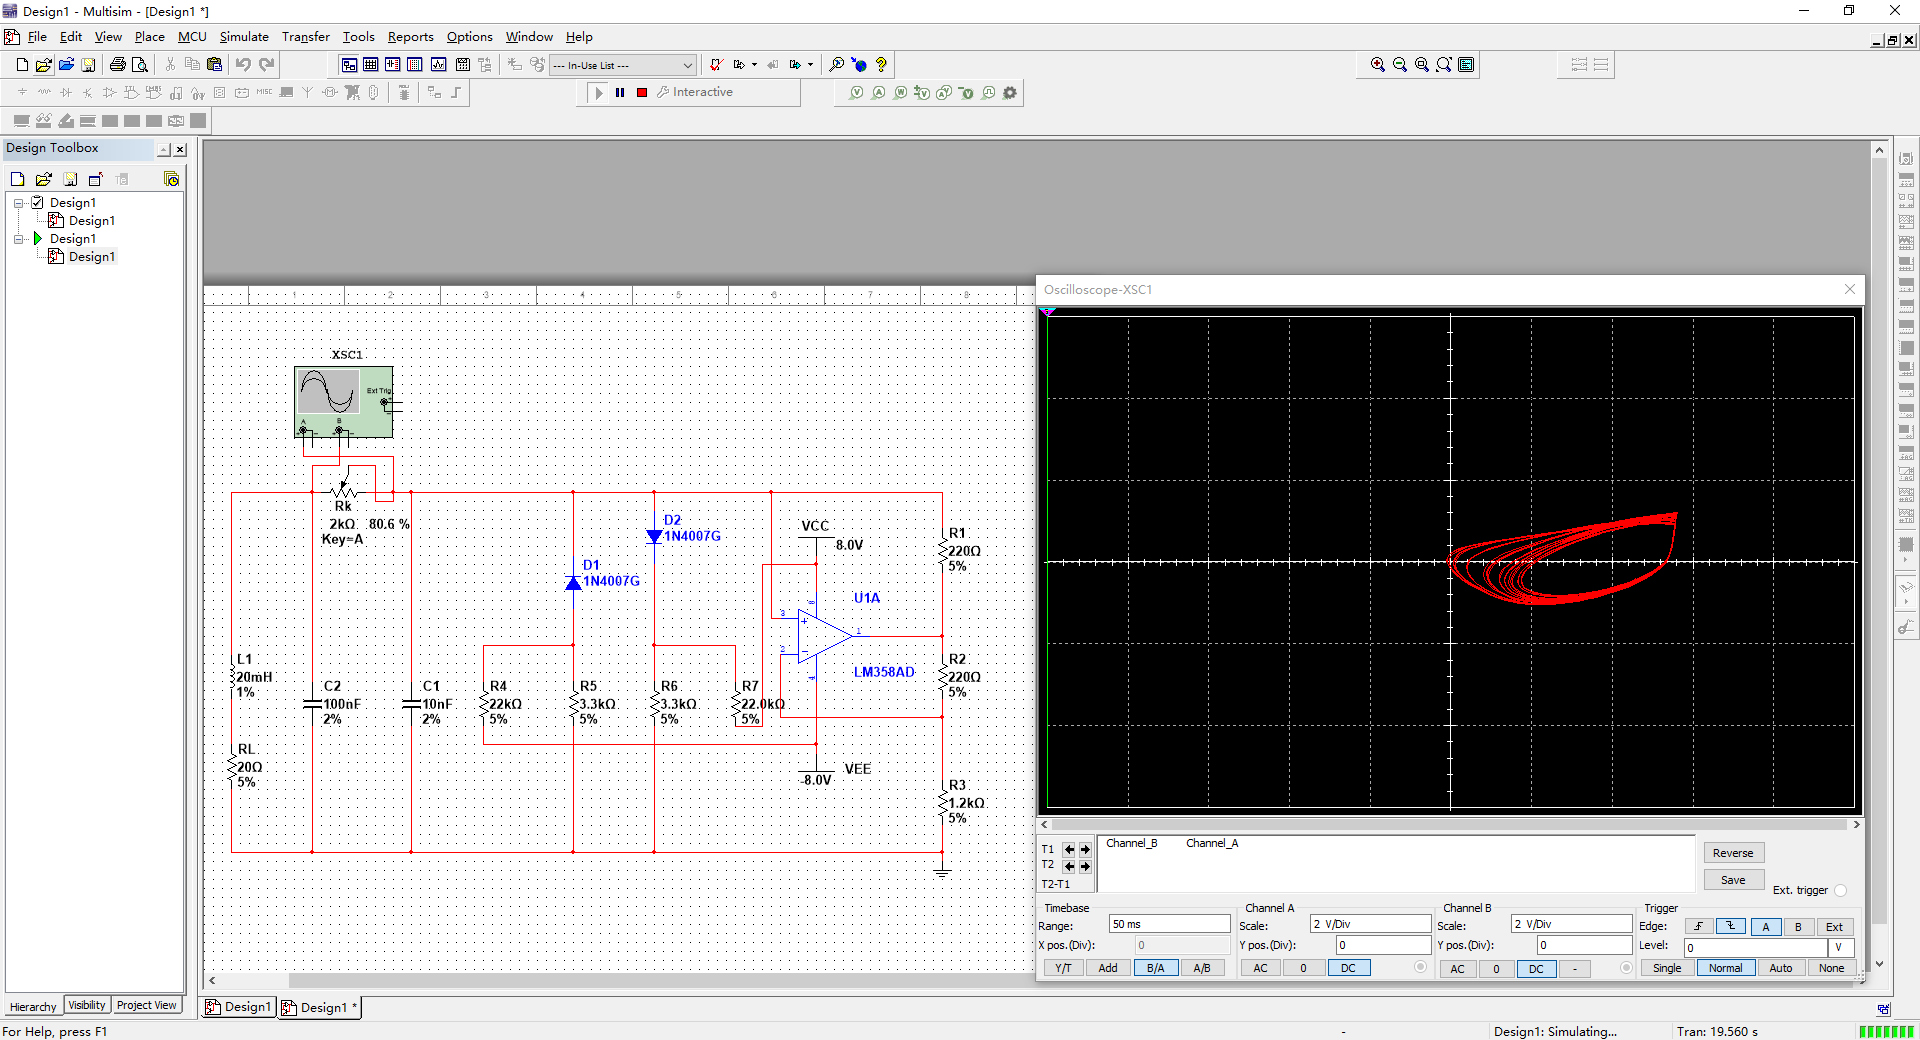
\includegraphics[width=0.3\textwidth]{attachments/fig.2.2.1st.png}
				}
				\caption{\textbf{Chua's circuit II, simulation results}}
				\label{fig.2.2}
			\end{figure*}
		
			\subsubsection{Experiment}
			Finally, based on the results of numerical calculation and simulation, we built the real-world circuits (Fig. \ref{fig.3.0})  
			and adjust the resistance value to obtaine the oscillation patterns on VirtualBench. Results are shown as Fig. \ref{fig.3.1} and Fig. \ref{fig.3.2}
			Interestingly, different from the simulation results, we successfully obtained all the five patterns in the second circuit(Fig. \ref{fig.1.2}),
			while the pattern of second attractor was missing in the first circuit (Fig. \ref{fig.1.1}).
			We hypothesize that this might be ascribed to the additional influence of the wires and the breadboard on the oscillation state of the systems.
			
			\begin{figure*}[htbp]
				\centering
				\subfloat[Chua's Circuit I]{
				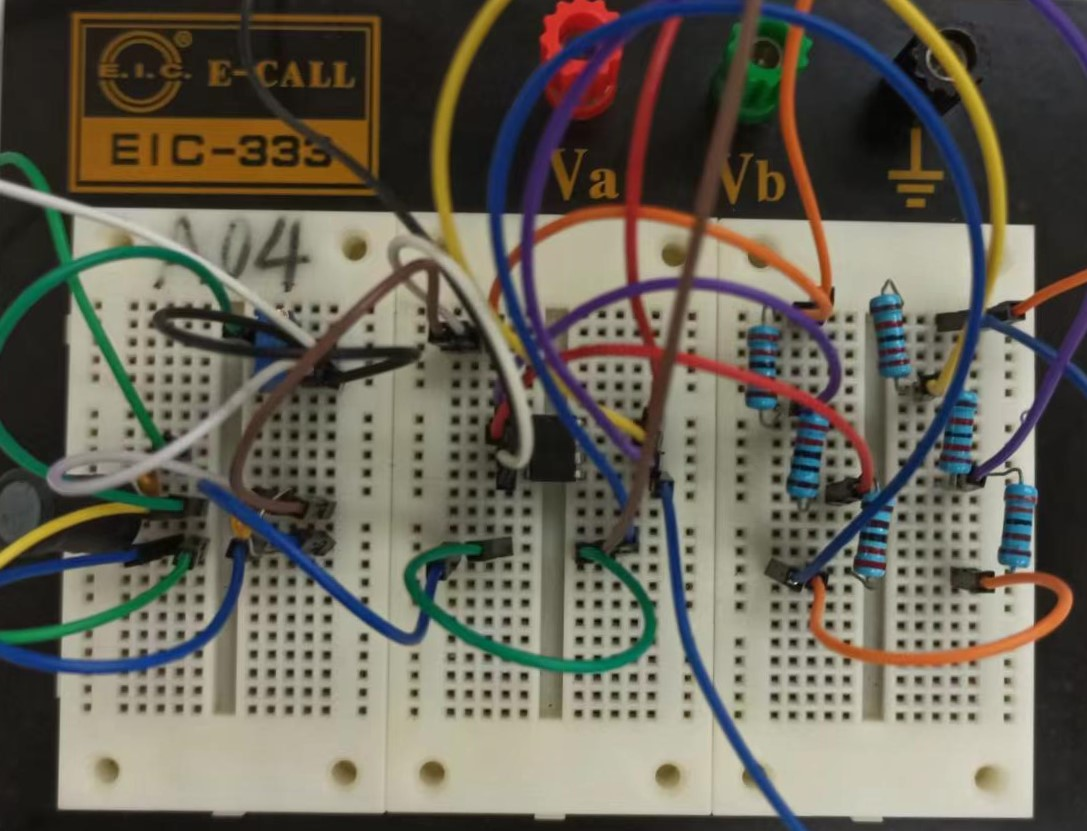
\includegraphics[width=0.4\textwidth]{attachments/fig.3.0.1.jpg}
				}
				\subfloat[Chua's Circuit II]{
				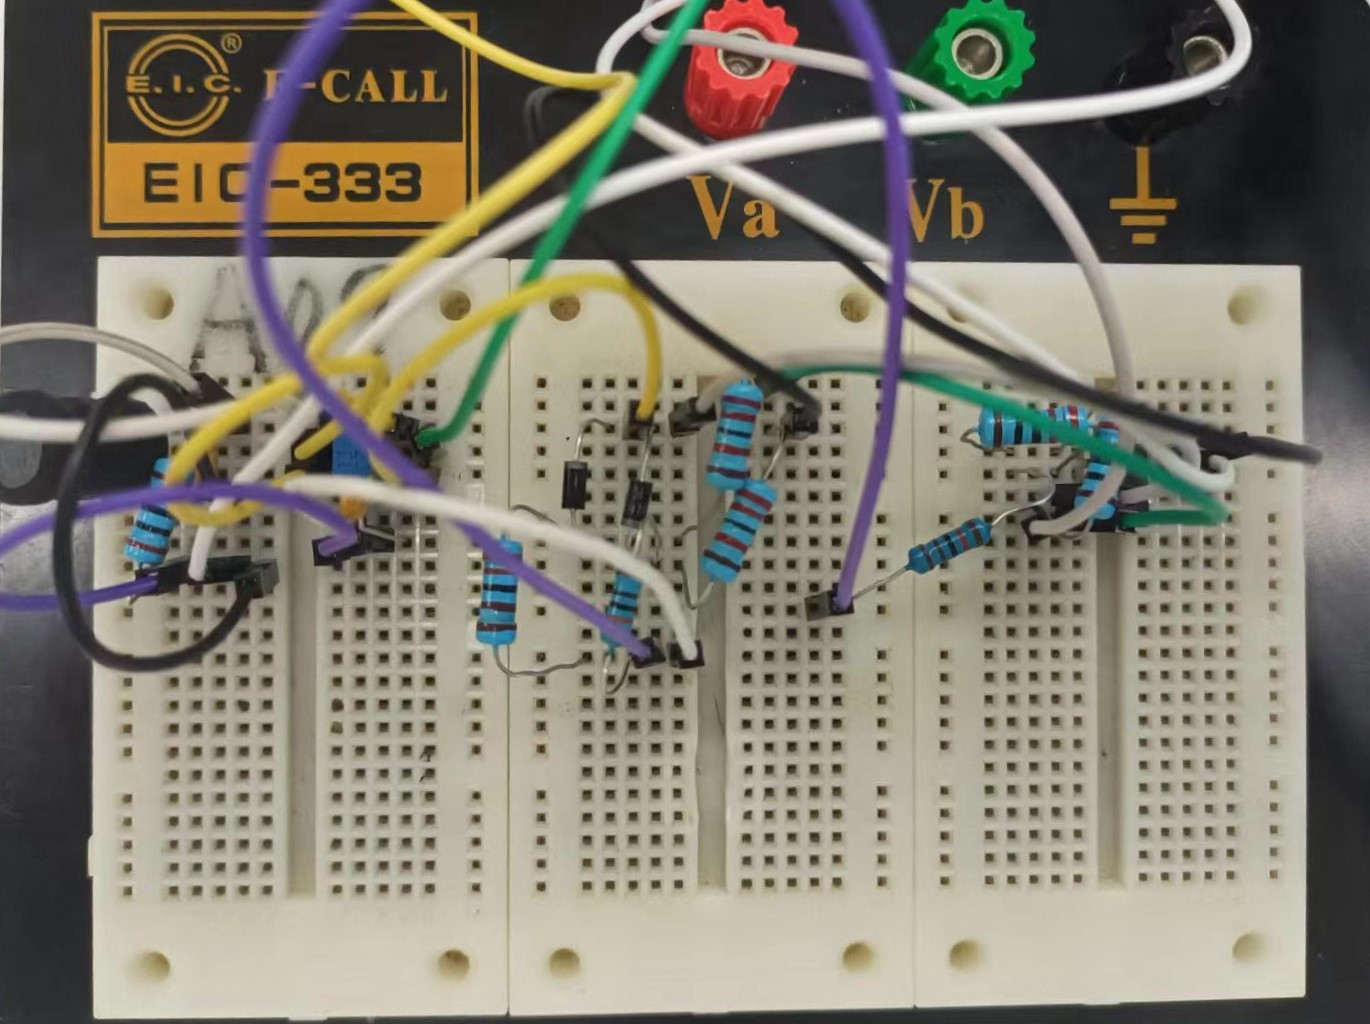
\includegraphics[width=0.4\textwidth]{attachments/fig.3.0.2.jpg}
				}
				\caption{\textbf{Chua's Circuit}}
				\label{fig.3.0}
			\end{figure*}


			\begin{figure*}[htbp]
				\centering
				\subfloat[line]{
				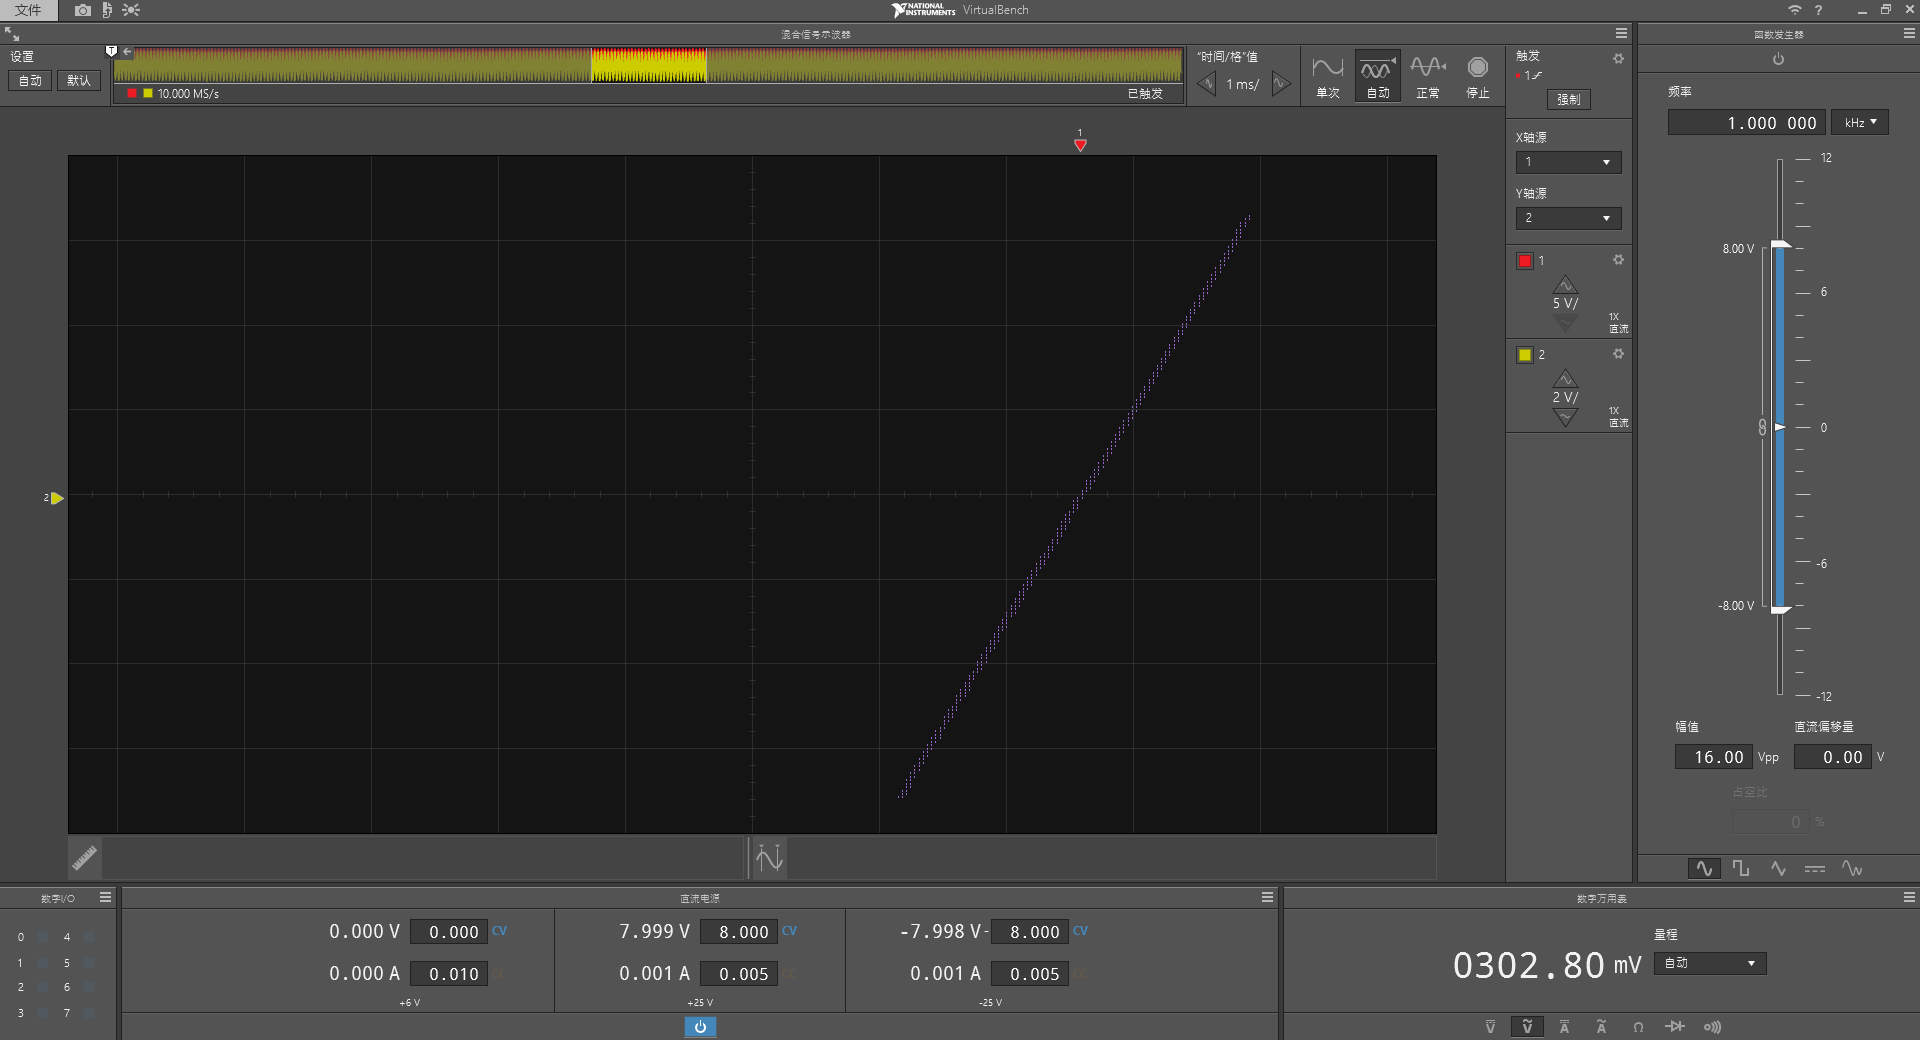
\includegraphics[width=0.3\textwidth]{attachments/fig.3.1.line.png}
				}
				\subfloat[limit ring]{
				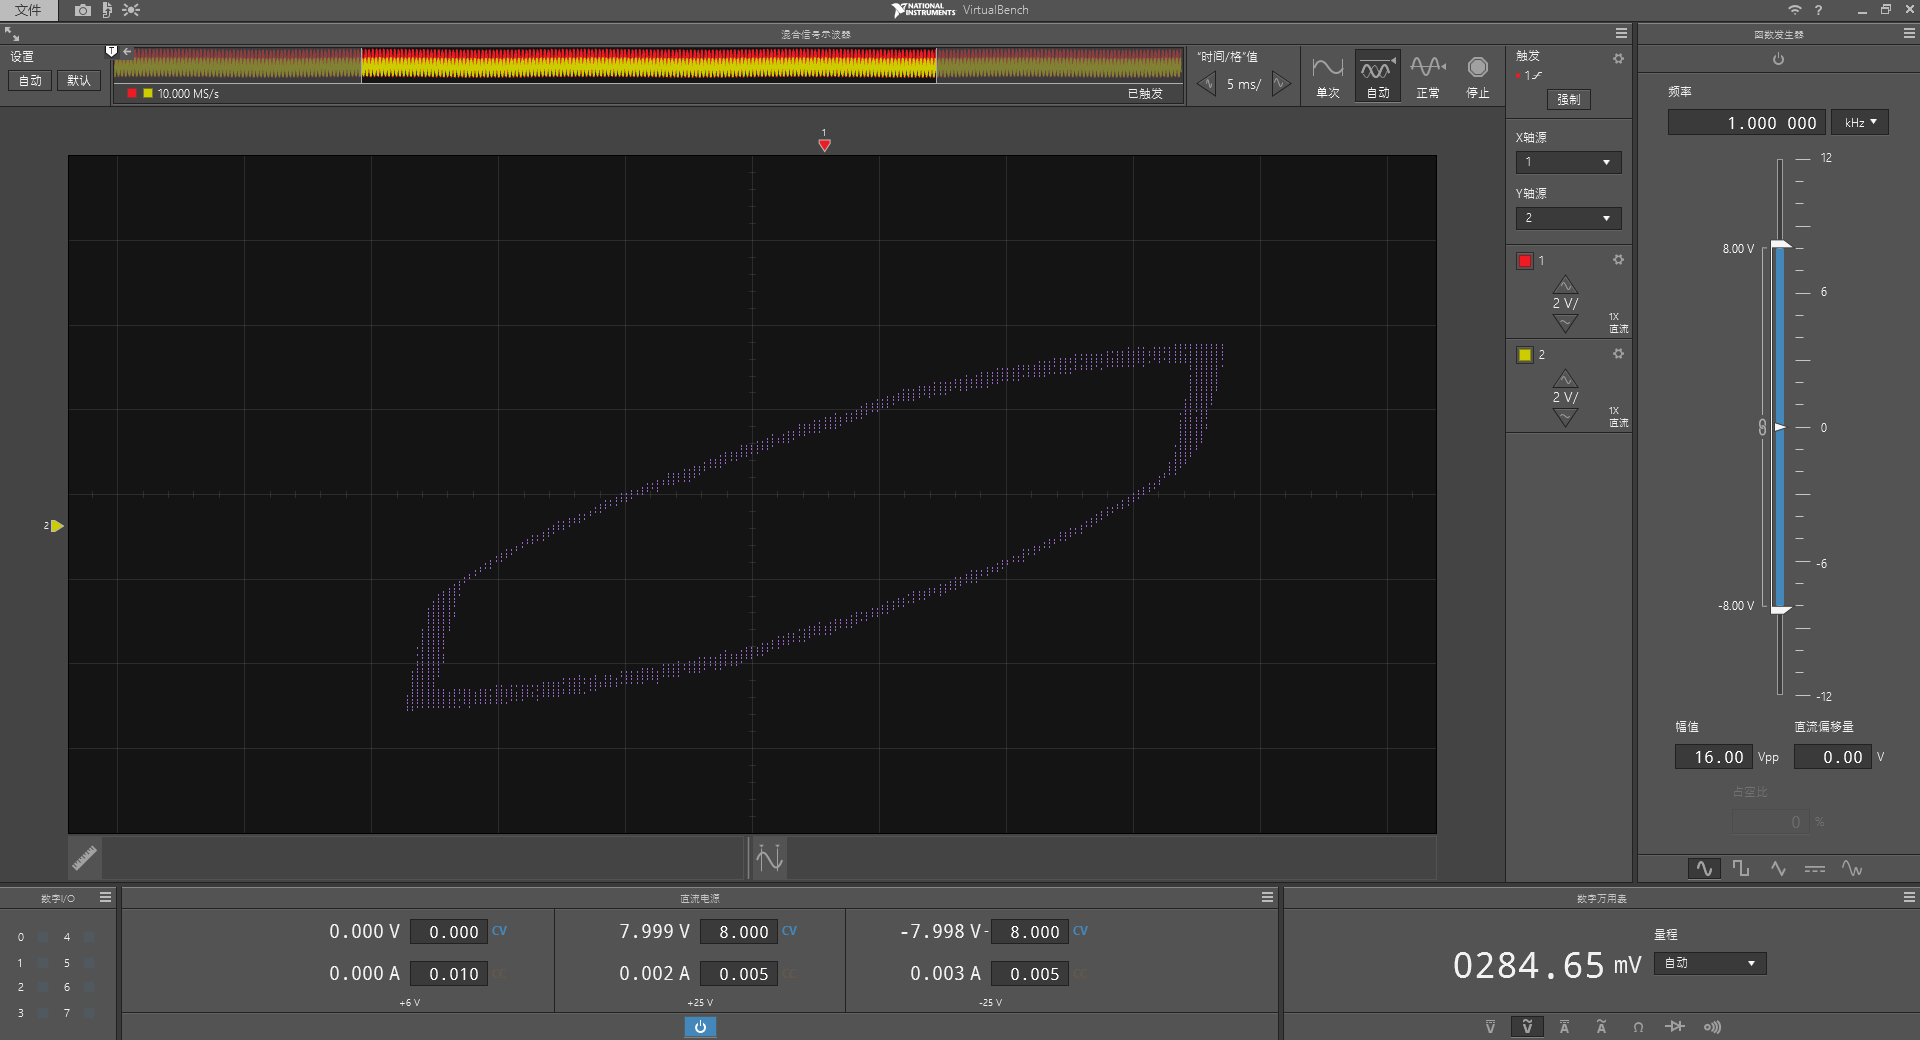
\includegraphics[width=0.3\textwidth]{attachments/fig.3.1.limit ring.png}
				}

				\subfloat[double attractors]{
				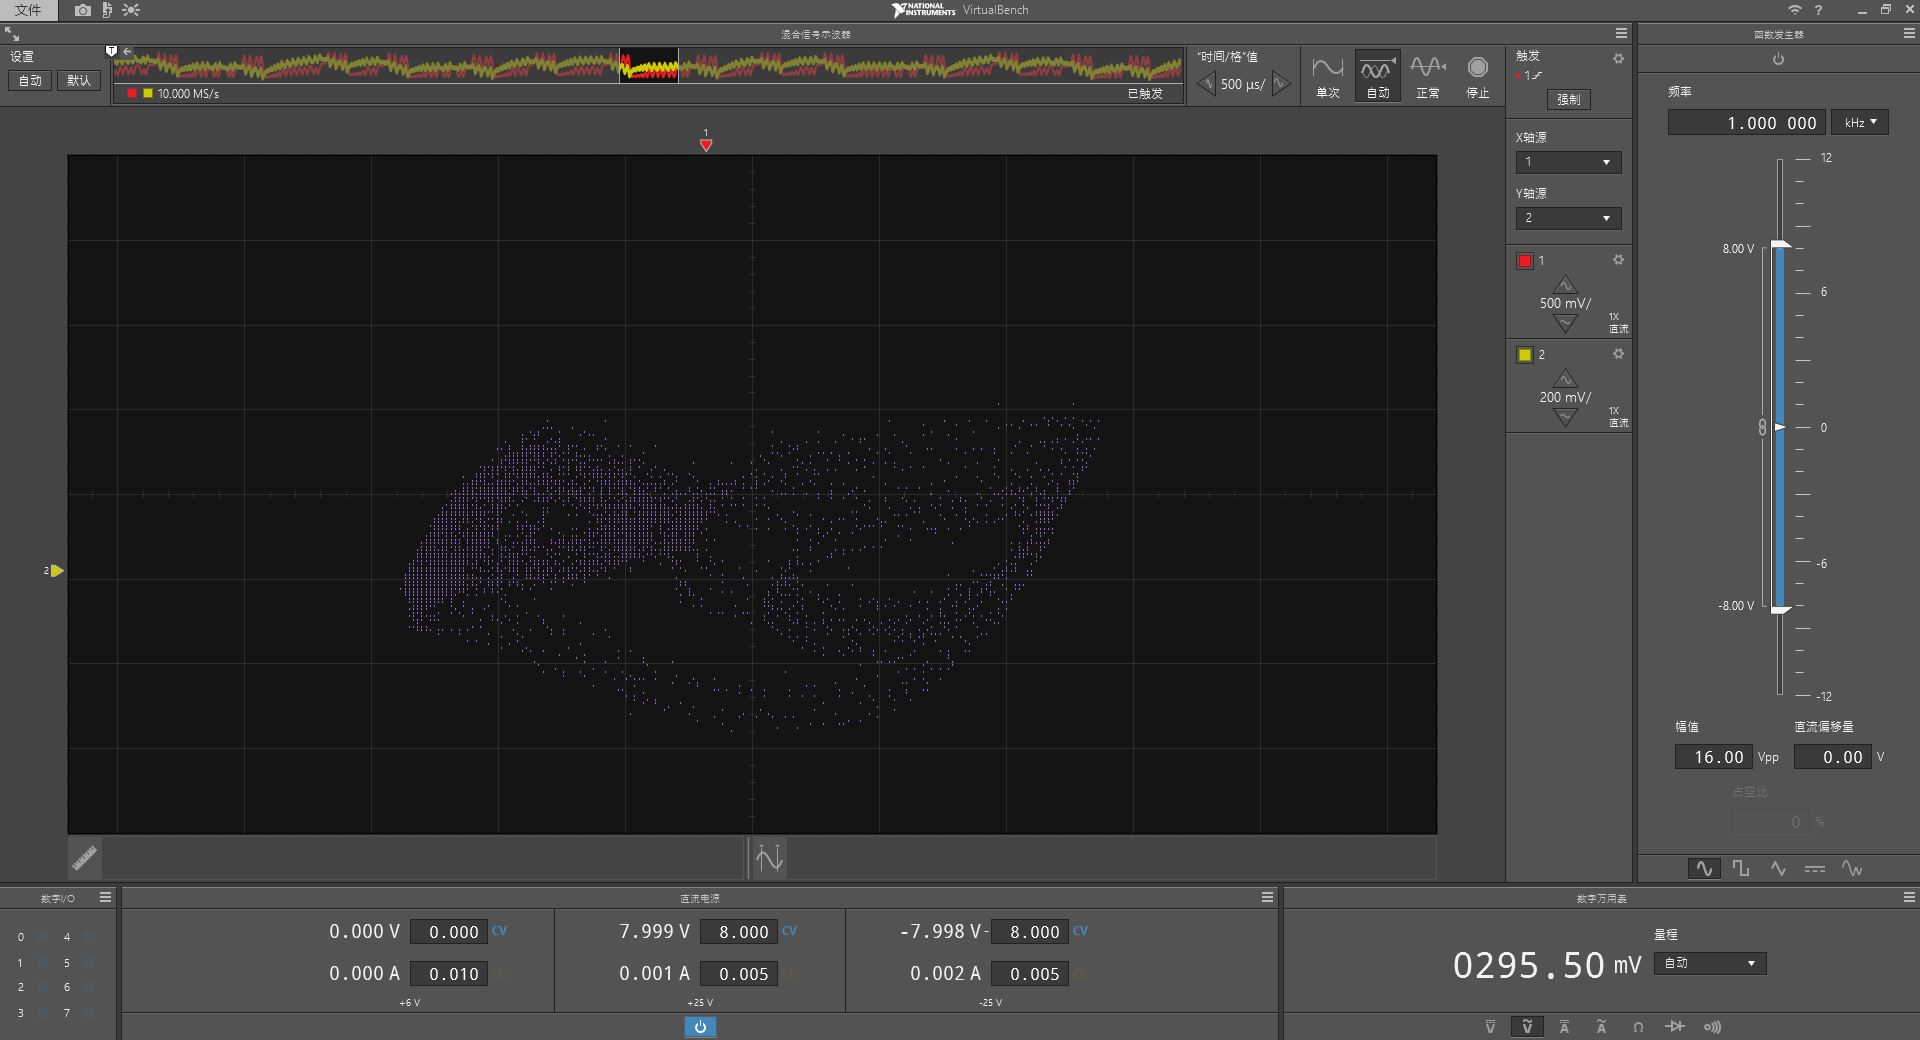
\includegraphics[width=0.3\textwidth]{attachments/fig.3.1.double attractors.png}
				}
				\subfloat[1st single attractor]{
				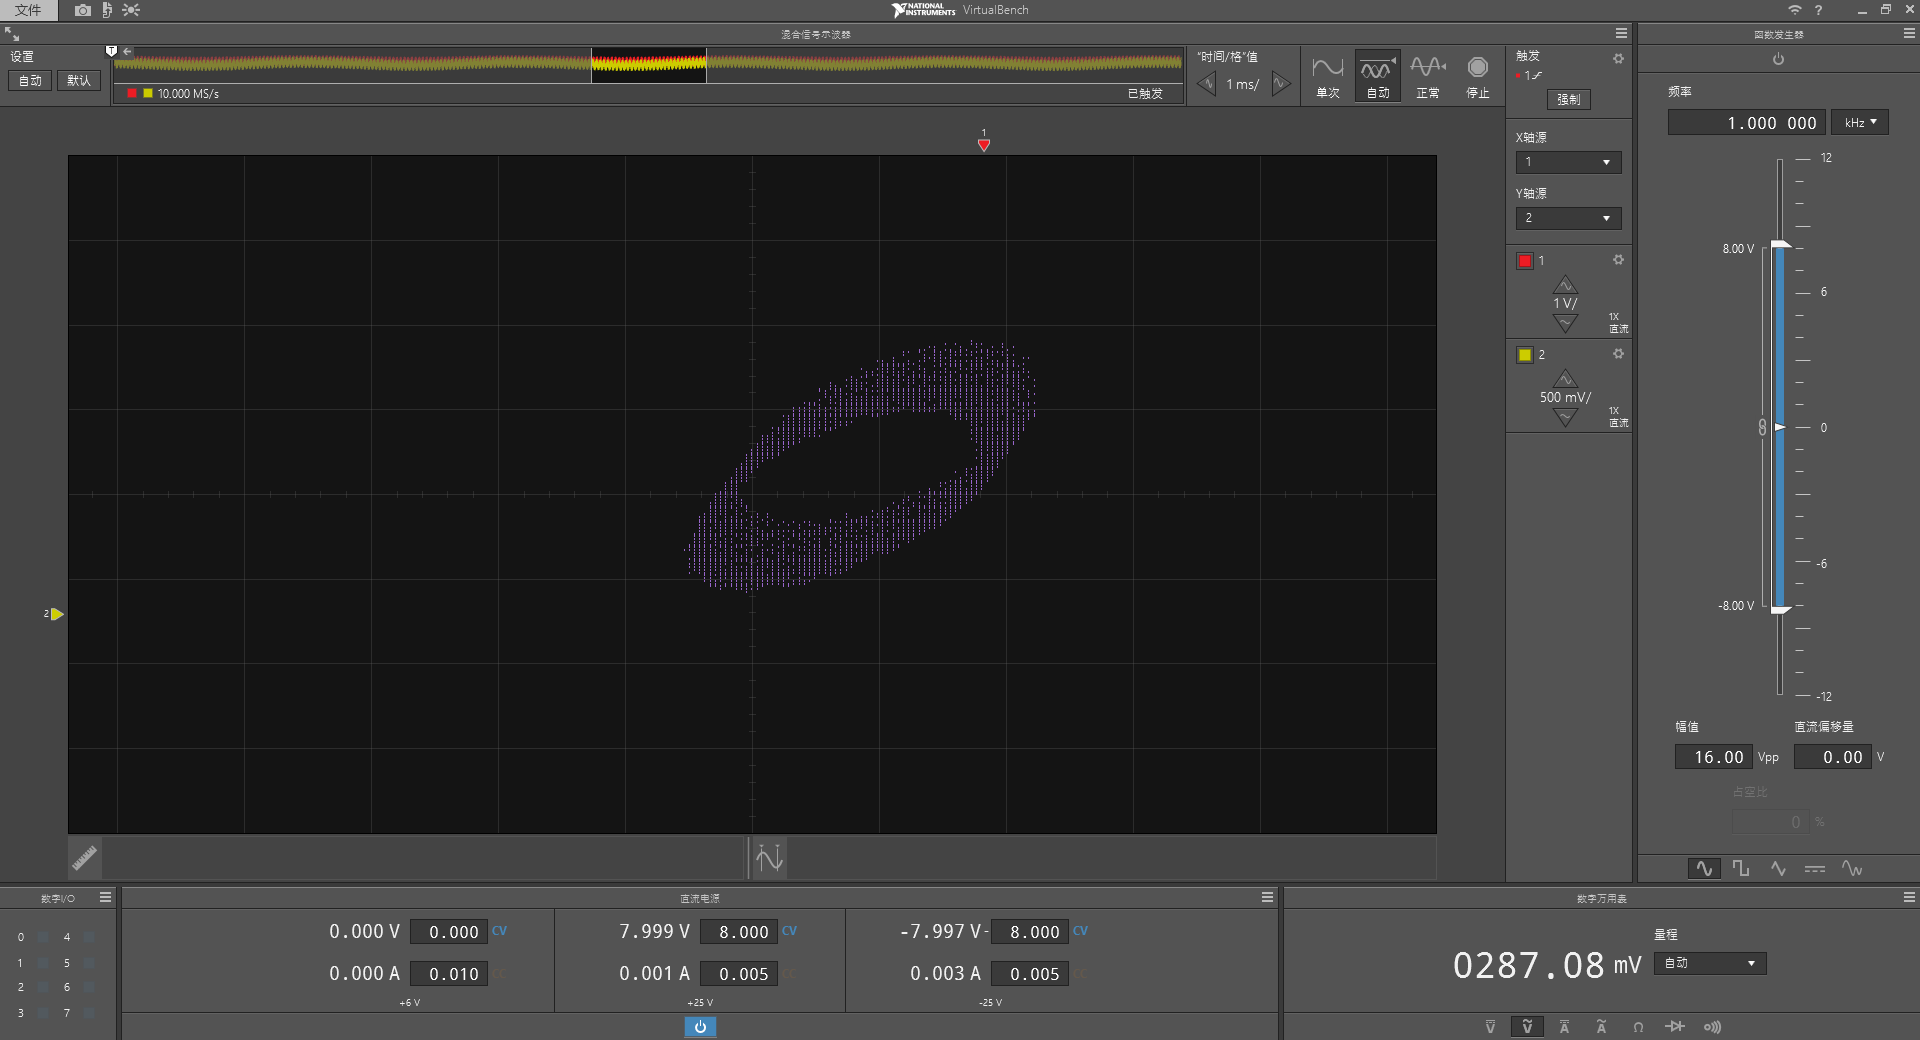
\includegraphics[width=0.3\textwidth]{attachments/fig.3.1.1st.png}
				}
				\caption{\textbf{Chua's circuit I, real-world experiment results}}
				\label{fig.3.1}
			\end{figure*}

			\begin{figure*}[htbp]
				\centering
				\subfloat[line]{
				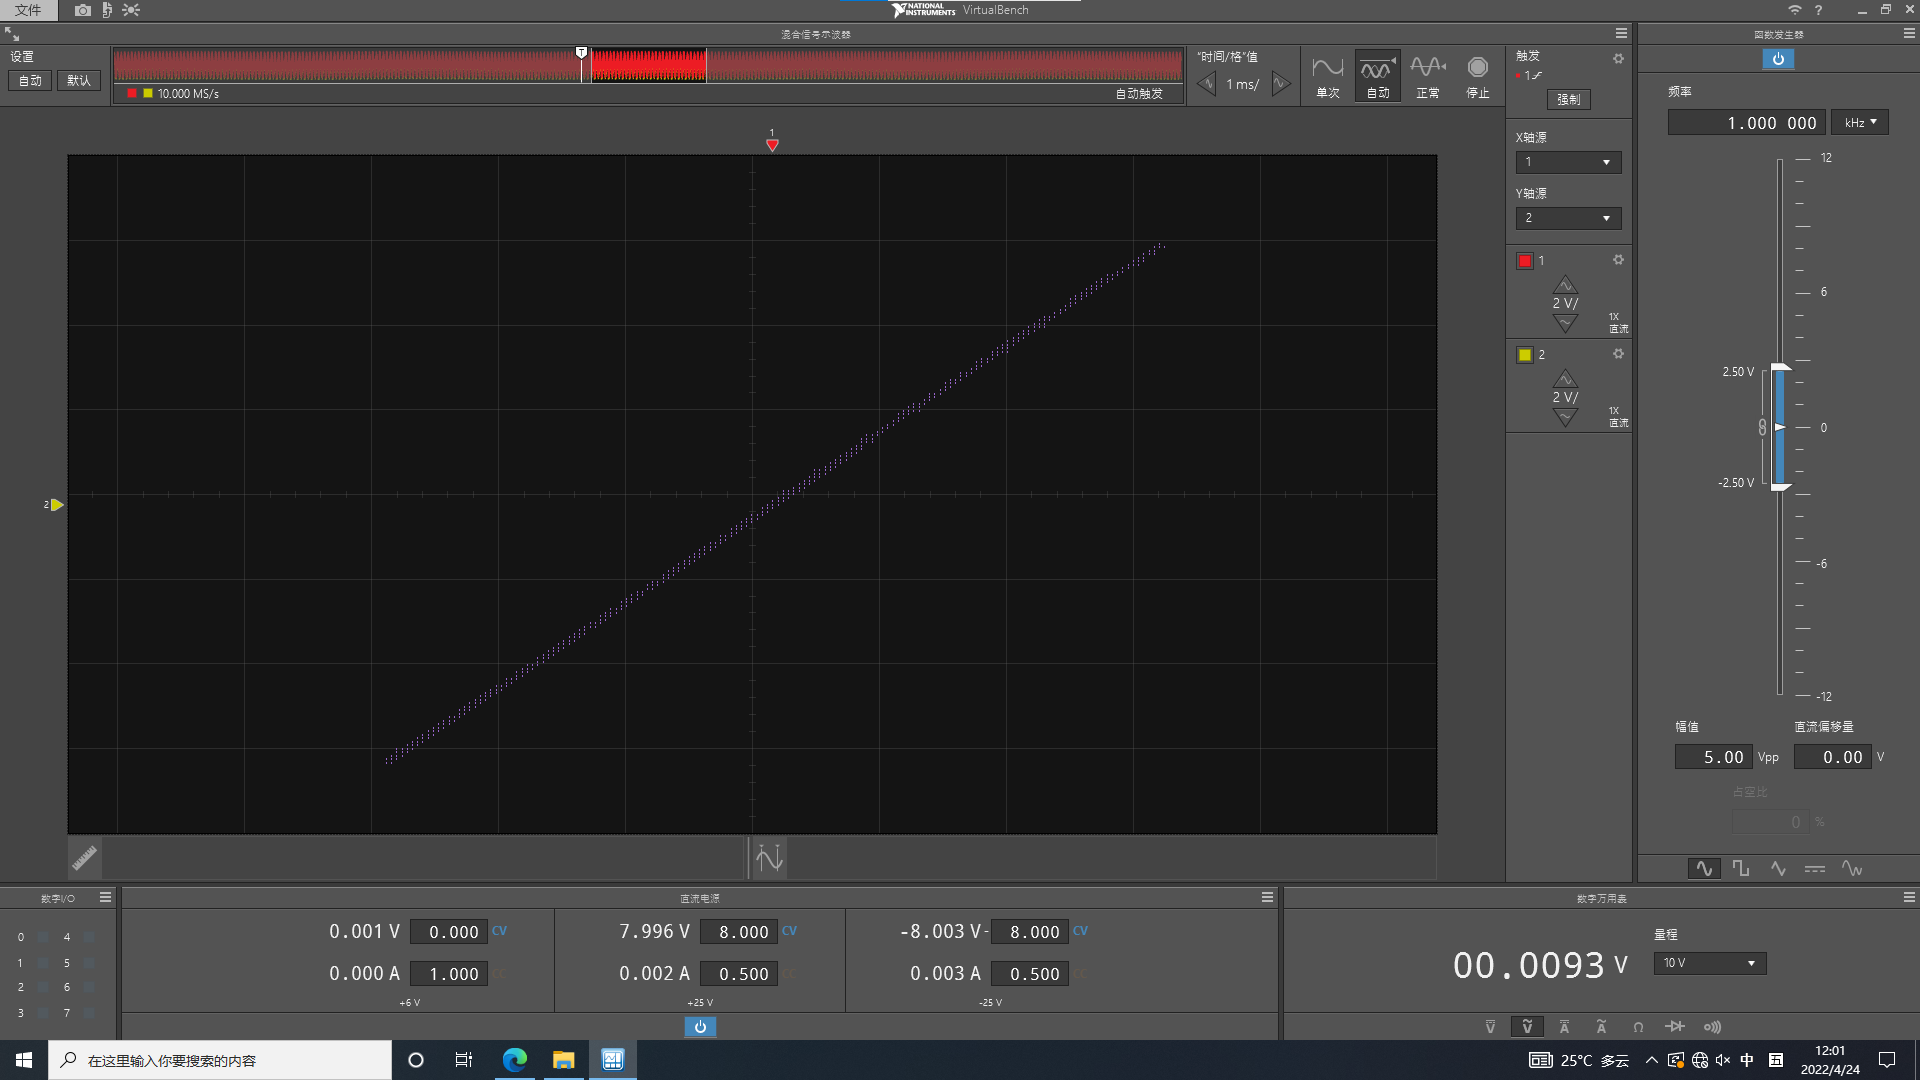
\includegraphics[width=0.3\textwidth]{attachments/fig.3.2.line.png}
				}
				\subfloat[limit ring]{
				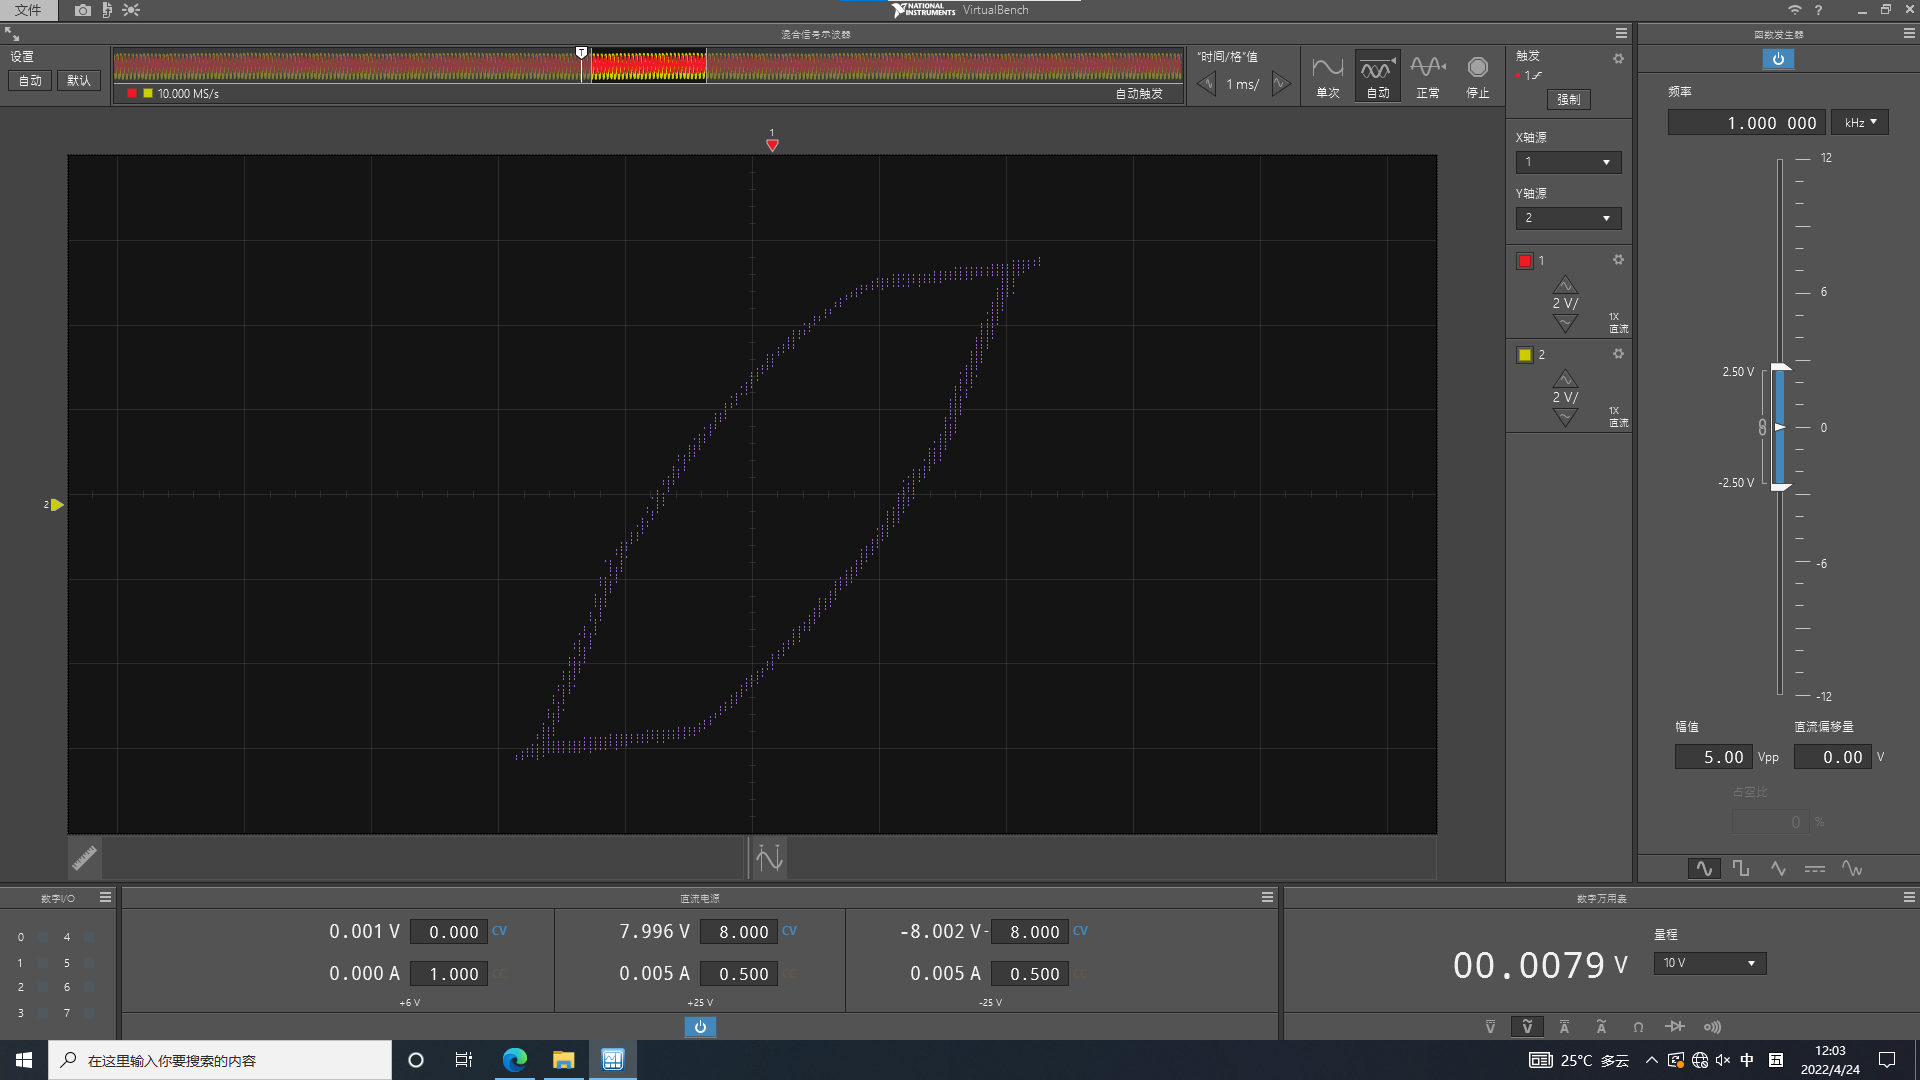
\includegraphics[width=0.3\textwidth]{attachments/fig.3.2.limit ring.png}
				}
				
				\subfloat[double attractors]{
				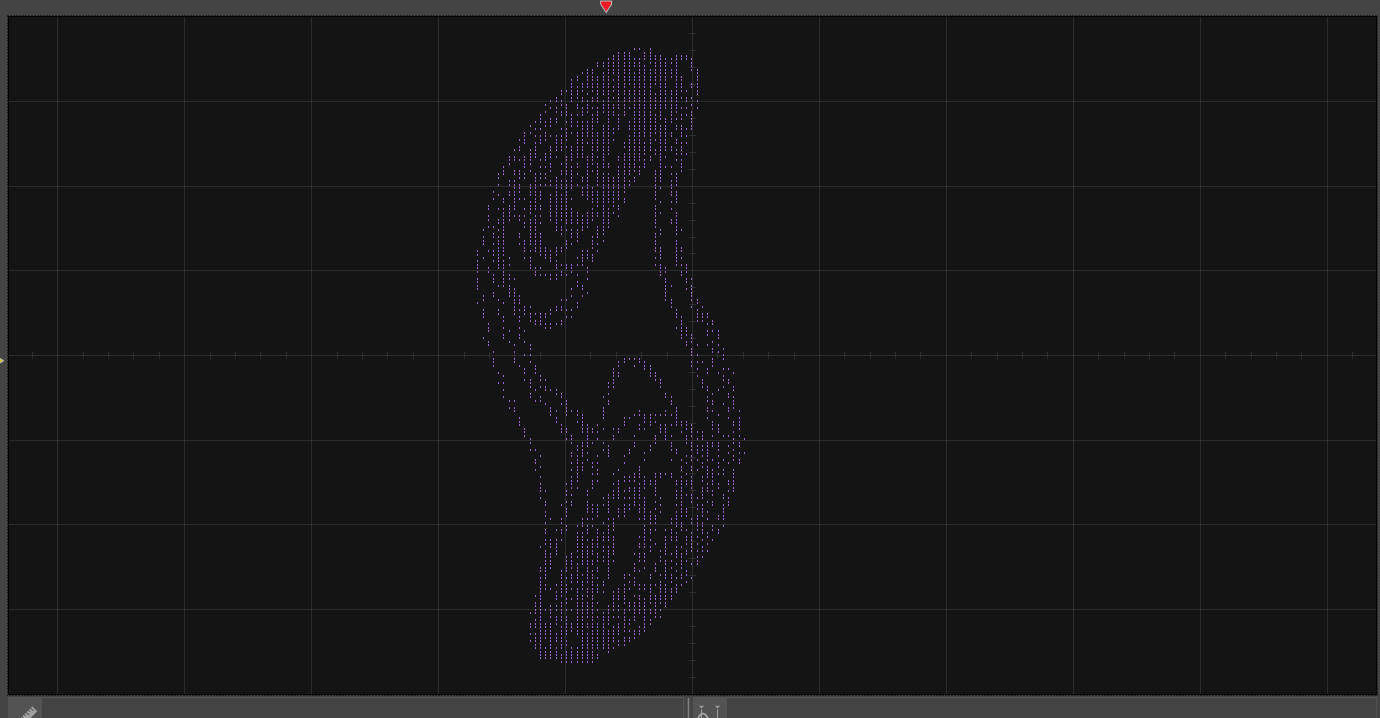
\includegraphics[width=0.3\textwidth]{attachments/fig.3.2.double attractors.png}
				}
				\subfloat[1st single attractor]{
				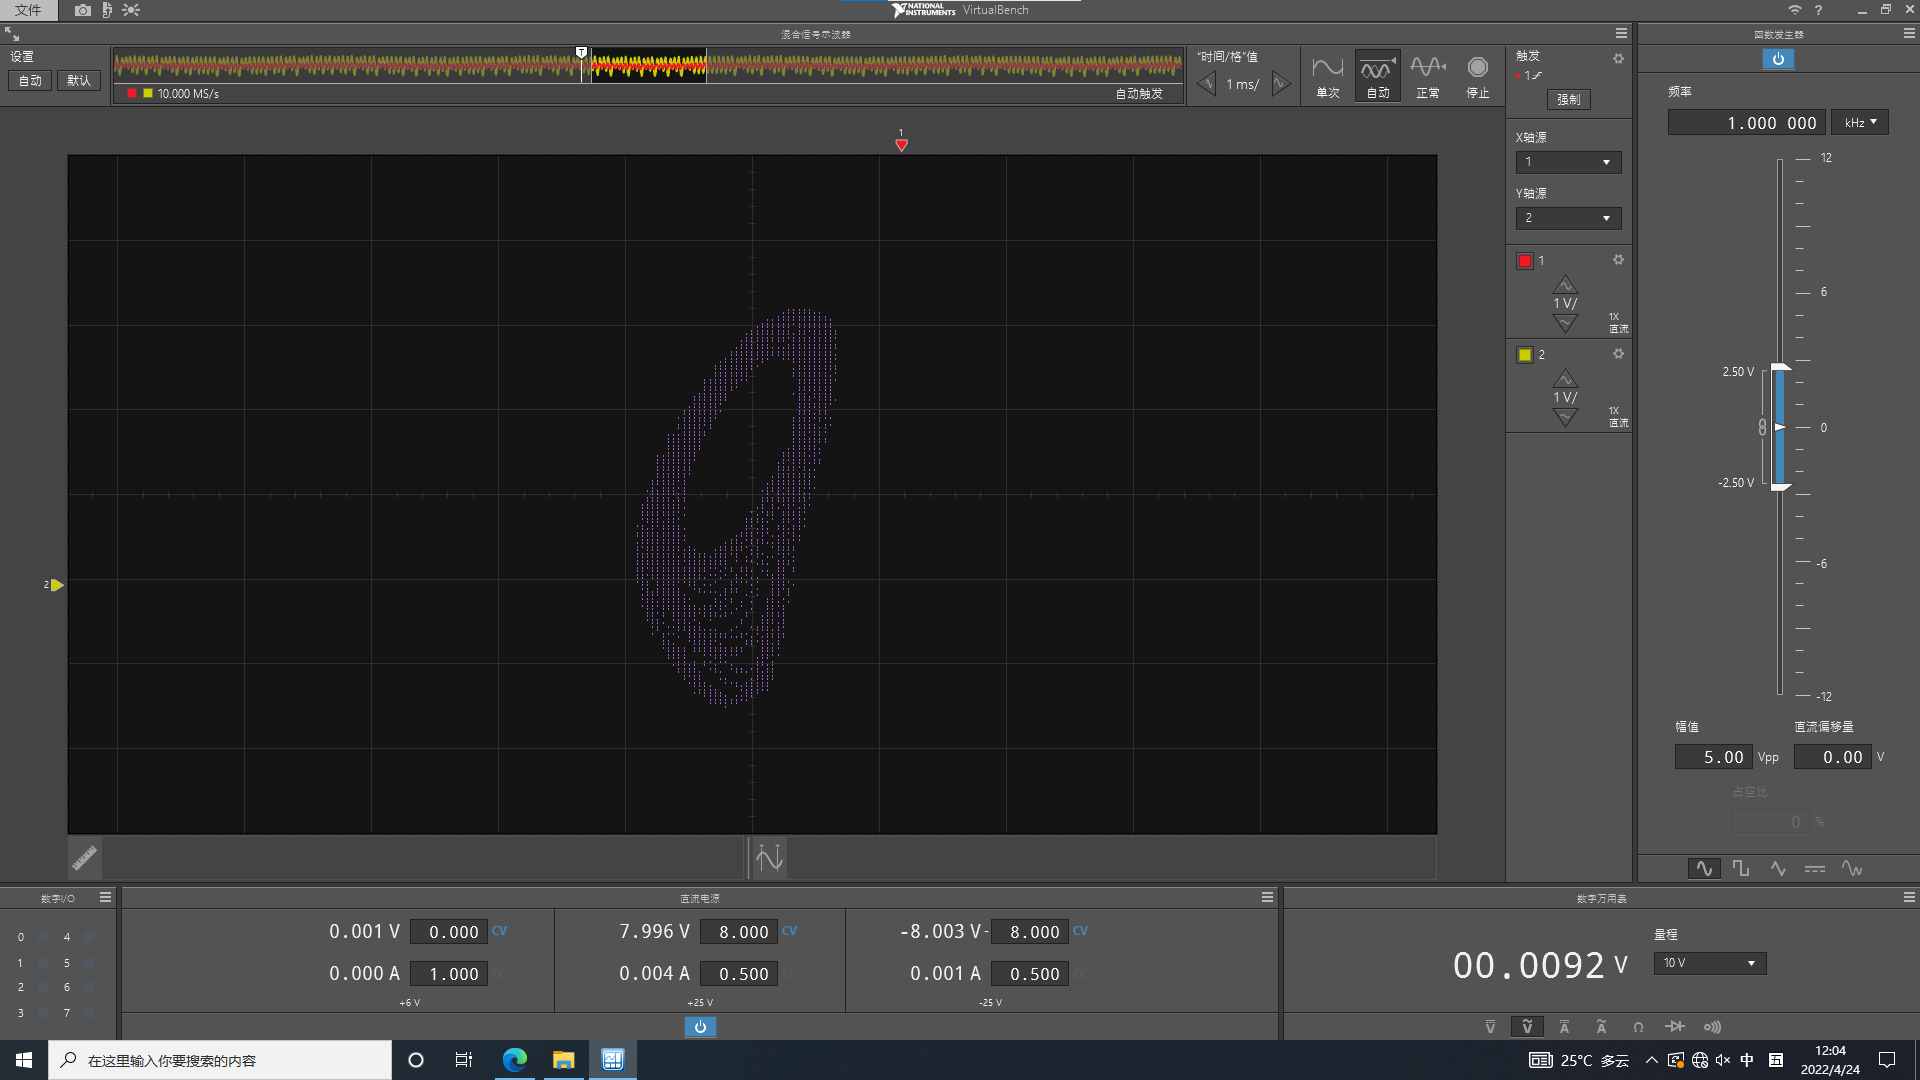
\includegraphics[width=0.3\textwidth]{attachments/fig.3.2.1st.png}
				}
				\subfloat[2nd single attractor]{
				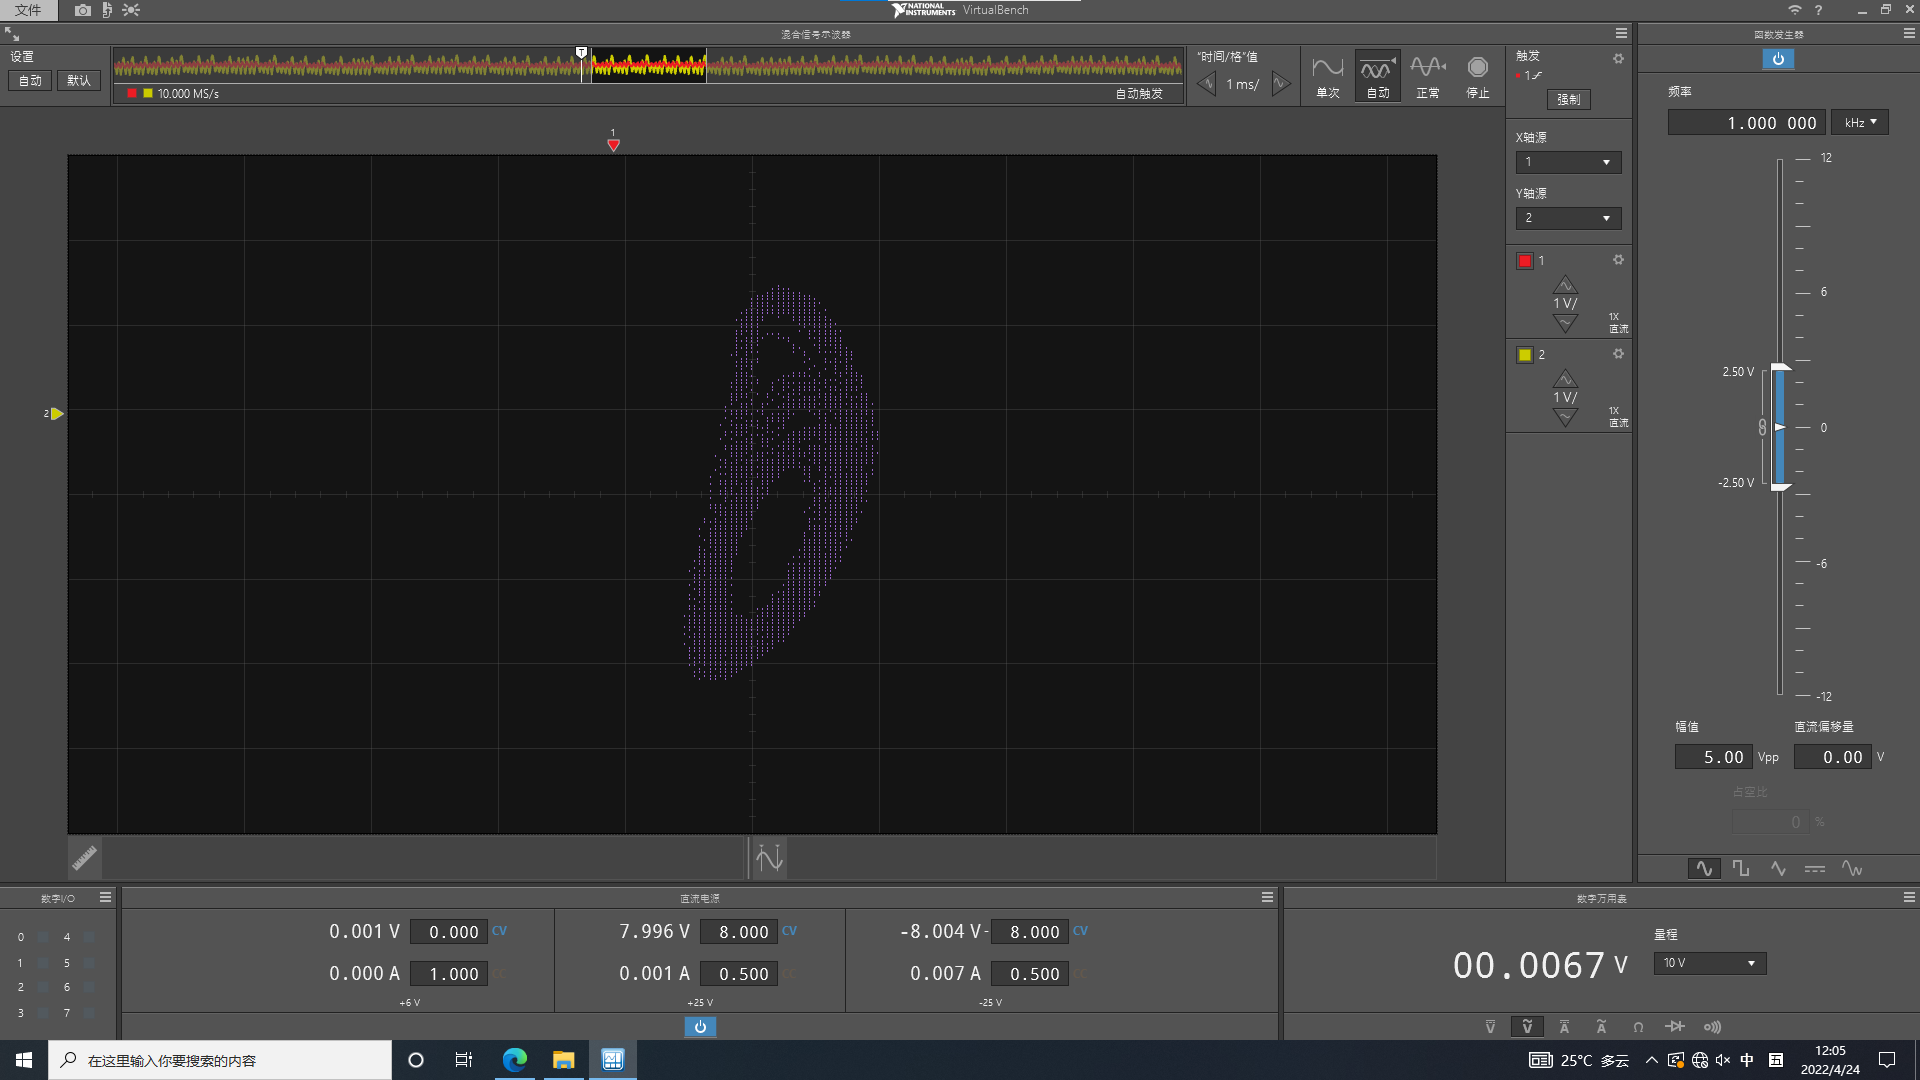
\includegraphics[width=0.3\textwidth]{attachments/fig.3.2.2nd.png}
				}
				\caption{\textbf{Chua's circuit II, real-world experiment results}}
				\label{fig.3.2}
			\end{figure*}

	\subsection{Lorentz's circuit}
		\subsubsection{Numerical calculation}
		Different numerical solutions of chaotic oscillations were obtained by solving Eq. \ref{eq.2.1} with different parameters $P, \gamma, b$.
		We found that oscillation patterns generted by this circuit were impressively abundant. 
		As a representative oscillation state, the Lorentz's butterfly was generated and shown in Fig. \ref{fig.4.1}.

		The parameters are summarized in the Supplementary Information.

		A Jupyter Notebook including all codes for calculation and an interactive ipywidget which allows adjusting the parameters conveniently is available on \href{https://github.com/Zweig-Wong/SYSU-PHY-EXP/blob/main/C9-Chaotic_circuit/Lorentz/Calculation/Lorentz.ipynb}{https://github.com/Zweig-Wong/SYSU-PHY-EXP}
		\begin{figure*}[htbp]
			\centering
			\subfloat[Channel]{
			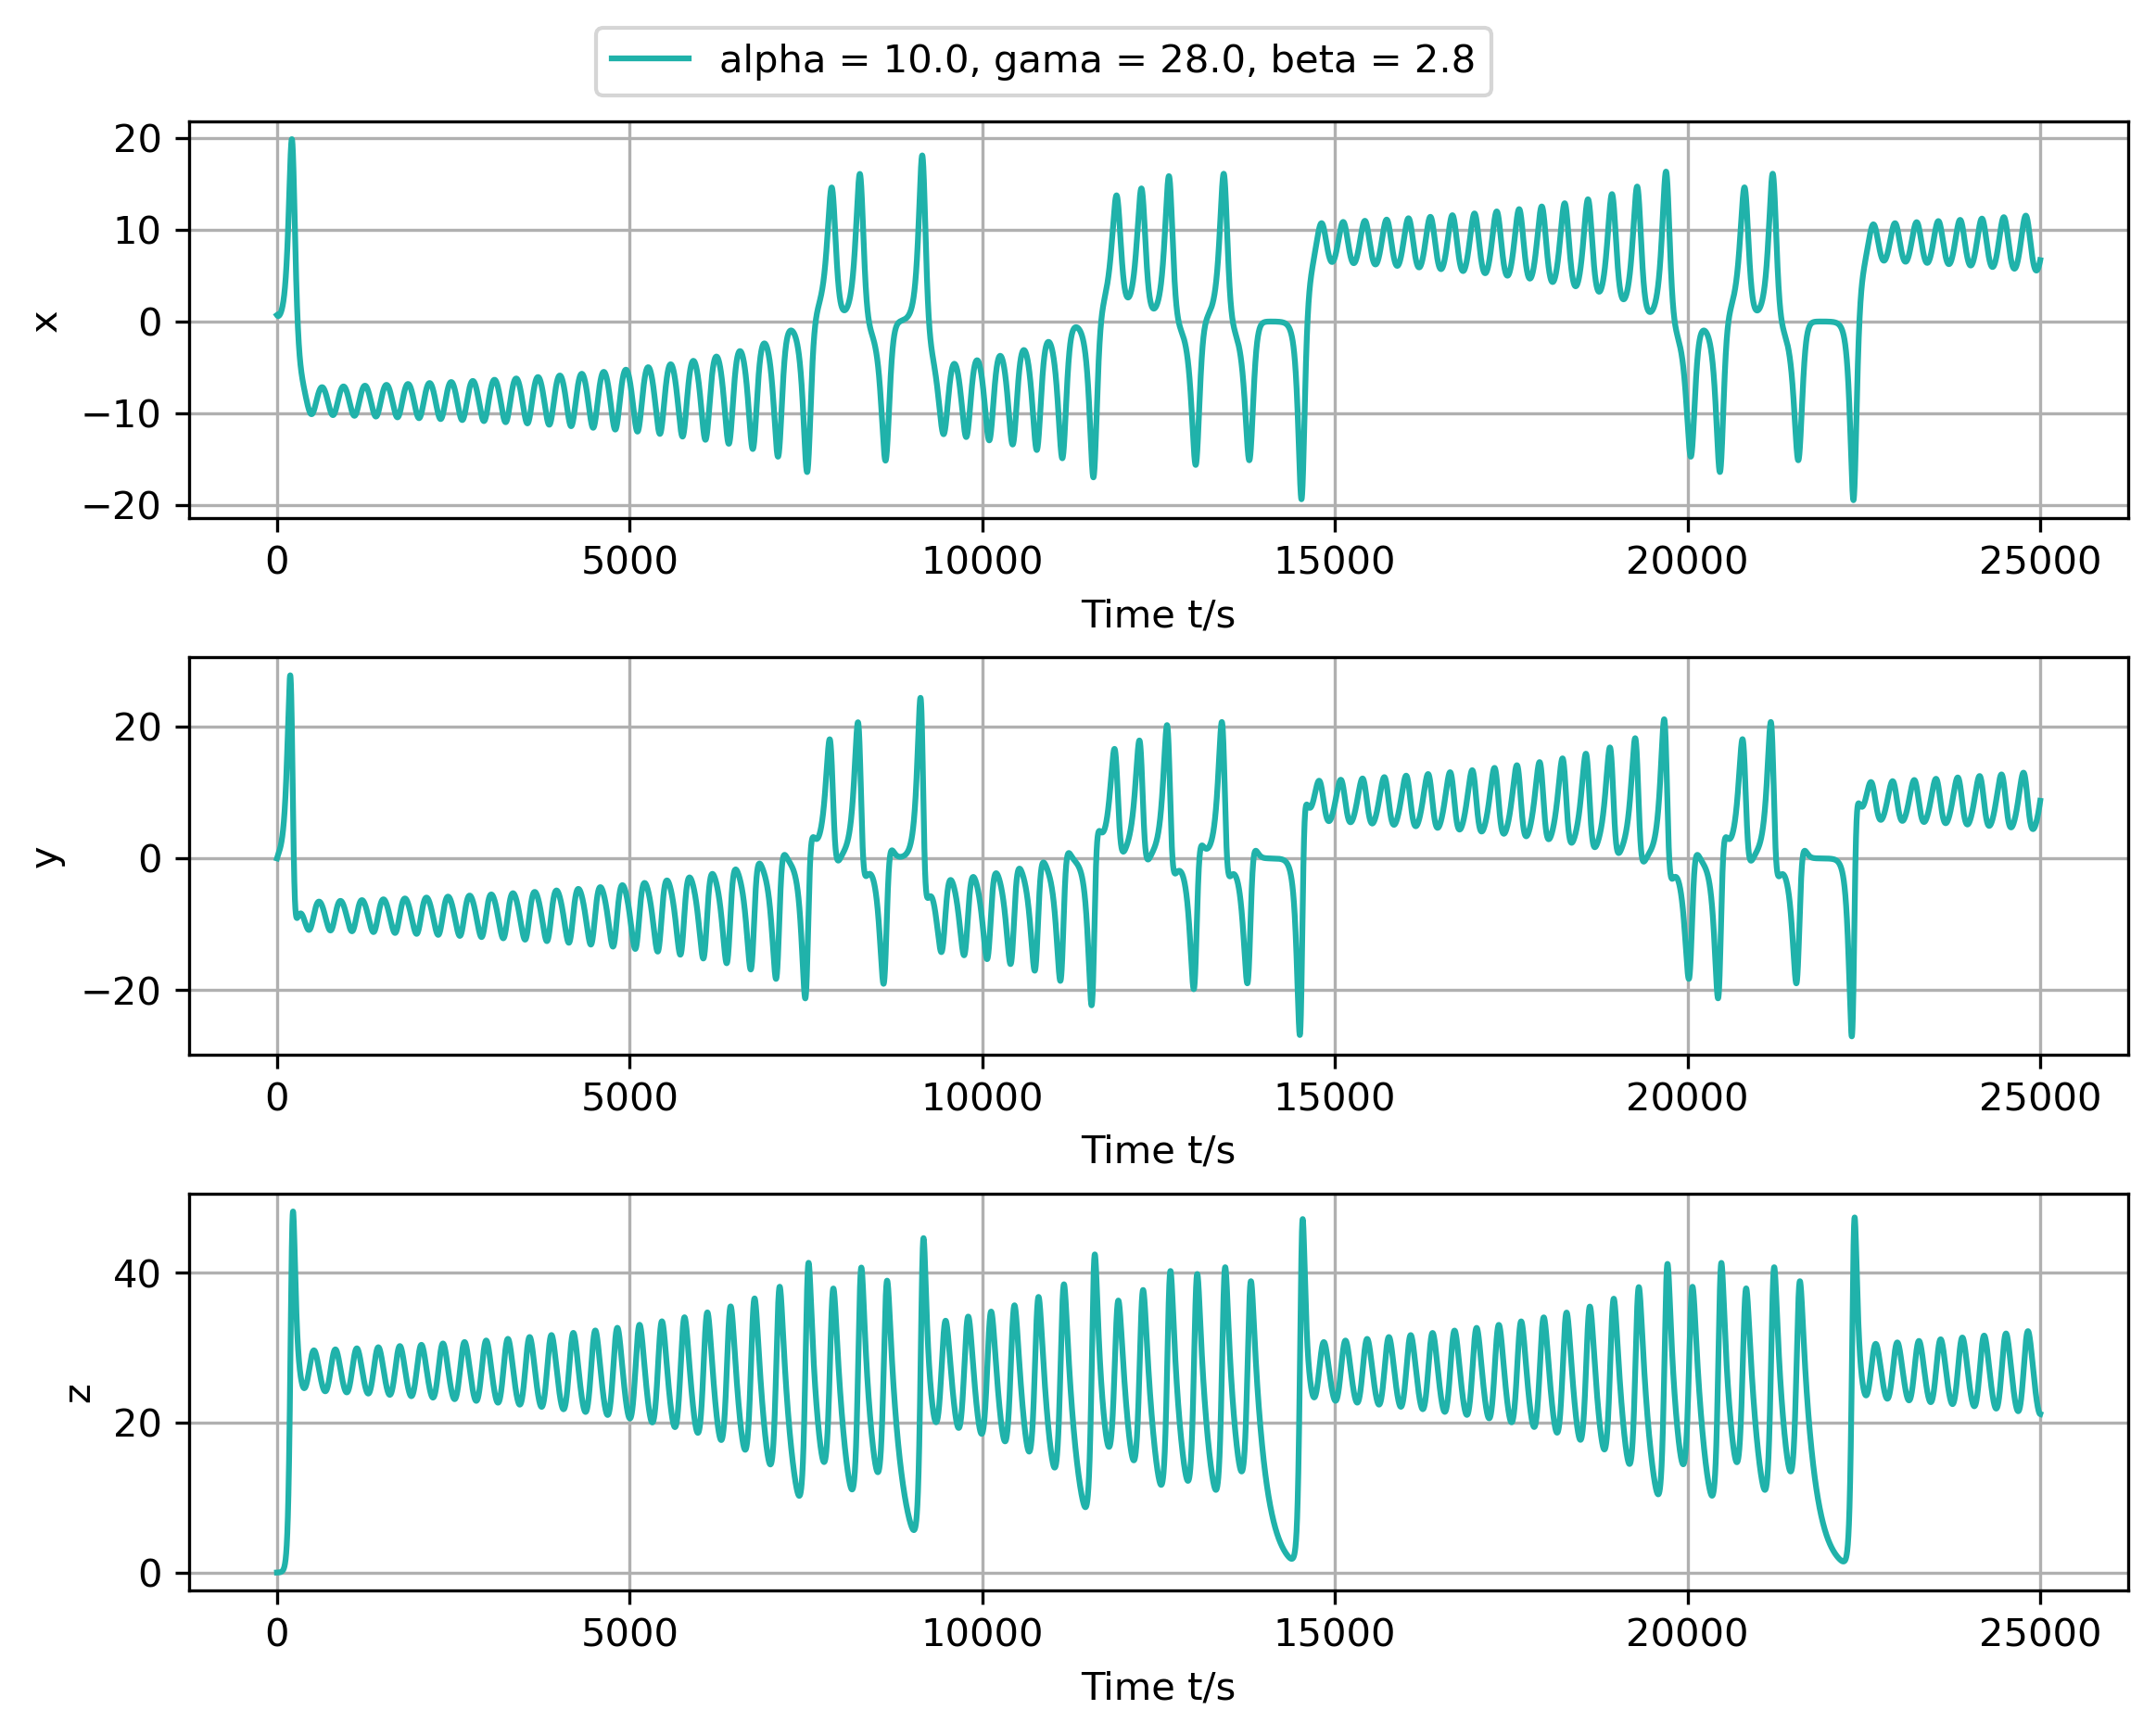
\includegraphics[width=0.3\textwidth]{attachments/fig.4.1.wave.png}
			}
			\subfloat[3d trace]{
			\includegraphics[width=0.3\textwidth]{attachments/fig.4.1.3d.png}
			}
			
			\subfloat[x-y plain]{
			\includegraphics[width=0.3\textwidth]{attachments/fig.4.1.x-y.png}
			}
			\subfloat[x-z plain]{
			\includegraphics[width=0.3\textwidth]{attachments/fig.4.1.x-z.png}
			}
			\subfloat[y-z plain]{
			\includegraphics[width=0.3\textwidth]{attachments/fig.4.1.y-z.png}
			}
			\caption{\textbf{Numerical calculation of Lorentz's circuit, Lorentz butterfly}}
			\label{fig.4.1}
		\end{figure*}

		\subsubsection{Simulation}
		Then, we simulated the Lorentz's circuit on the LTspice platform, and successfully obtained the Lorentz's butterfly
		by preciously adjusting the parameters (See the Supplementary Information).
		\begin{figure*}[htbp]
			\centering
			\subfloat[x-y plain]{
			\includegraphics[width=0.3\textwidth]{attachments/fig.5.1.x-y.png}
			}
			\subfloat[x-z plain]{
			\includegraphics[width=0.3\textwidth]{attachments/fig.5.1.x-z.png}
			}
			\subfloat[y-z plain]{
			\includegraphics[width=0.3\textwidth]{attachments/fig.5.1.y-z.png}
			}
			\caption{\textbf{Simulation of Lorentz's circuit, Lorentz butterfly}}
			\label{fig.5.1}
		\end{figure*}


%%end-------------------Result-----------------------%%

%%begin-------------------Conclusion and Discussion-----------------------%%
\section{Conclusion and Discussion}
	\subsection{Conclusion}
		In this research, we investigated different oscillation patterns of Chua's and Lorentz's chaotic circuits by conducting numerical calculations, simulations and real-world circuit experiments.
		We found that with different initial parameters, the chaotic states of the system varied a lot, and the chaotic patterns were highly sensitive to the changes of parameters.
		The signals of chaotic oscillations, as illustrated in the results of the numerical calculation experiment, were continuous and limited.
		What's more, we also observed the pattern of double attractors in both Chua's and Lorentz's chaotic circuits, which is considered as the most famous typical chaotic pattern,
		This provided a strong evidence that the orbits in the phrase space are never repeat and ergodic, and they confines to a finite region and has stable and complex attractor.
		These findings were mutually verified in all experiments we have conducted, which revealed the general characteristics and principles of the chaotic systems.
		We believe that our findings on the nature of chaotic circuits can be properly further extended to other chaotic systems in different fields, 
		and our methods of building and exploring an analog circuit for a complex chaotic system might provide researchers in other fields with an instructive idea.
	\subsection{Known limitation}
		\begin{enumerate}[label=\arabic*.]
			\item Due to the limitation of available components, we did not build the real-world Lorentz's circuit and test its practicality. This might require further research.
			\item In Chua's circuit experiment, it is perplexing that the pattern of second single operator was sometimes missing. This might require further research.
		\end{enumerate}

%%end-------------------Conclusion and Discussion-----------------------%%

%%begin--------------------Reference------------------------%%
\printbibliography[title=Reference] 
%%end--------------------Reference------------------------%%
\end{document}